\documentclass[a4paper, notitlepage]{report}

% load packages
\usepackage[english]{babel}
\usepackage[toc, page]{appendix}
\usepackage{geometry, mathtools, amsthm, amsmath, enumitem, float, dirtytalk, graphicx, textcomp, amssymb, cancel, hyperref, IEEEtrantools, mathrsfs, xfrac, pgfplots, bbding, titlepic, cleveref, bm, stmaryrd}

% layout
\geometry{margin=1in}

% paths
\graphicspath{ {./images/} }

% tikz  from first notes
\usepackage{tikz, tikz-cd}
\usetikzlibrary{matrix, calc, positioning, decorations.markings, decorations.pathmorphing, decorations.pathreplacing}
\usetikzlibrary{arrows,cd}
\usetikzlibrary{positioning}
\tikzset{>=stealth}

% tikz from second notes
\usetikzlibrary{matrix,positioning,arrows,calc,decorations.pathmorphing,shapes}
\tikzset{snake it/.style={-stealth,
decoration={snake, 
    amplitude = .4mm,
    segment length = 2mm,
    post length=0.9mm},decorate}}

% extras
\theoremstyle{plain}
\newtheorem{definition}{Definition}[chapter]
\newtheorem{lemma}{Lemma}[chapter]
\newtheorem{theorem}{Theorem}[chapter]
\newtheorem{corollary}{Corollary}[chapter]
\newtheorem{proposition}{Proposition}[chapter]

\theoremstyle{remark}
\newtheorem{example}{Example}[chapter]
\newtheorem*{notation}{Notation}
\newtheorem{remark}{Remark}[chapter]
\newtheorem*{solution}{Solution}

%environment shortcuts 
\def\ba{\begin{array}}
\def\ea{\end{array}}
\def\bc{\begin{corollary}}
\def\ec{\end{corollary}}
\def\bd{\begin{definition}}
\def\ed{\end{definition}}
\def\ben{\begin{enumerate}}
\def\een{\end{enumerate}}
\def\bse{\begin{equation*}}
\def\ese{\end{equation*}}
\def\be{\begin{example}$ $\par\nobreak\ignorespaces}
\def\ee{\end{example}}
\def\bi{\begin{IEEEeqnarray*}}
\def\ei{\end{IEEEeqnarray*}}
\def\bit{\begin{itemize}}
\def\eit{\end{itemize}}
\def\bl{\begin{lemma}}
\def\el{\end{lemma}}
\def\bnn{\begin{notation}}
\def\enn{\end{notation}}
\def\bn{\begin{note}}
\def\en{\end{note}}
\def\bp{\begin{proposition}}
\def\ep{\end{proposition}}
\def\bq{\begin{proof}$ $\par\nobreak\ignorespaces}
\def\eq{\end{proof}}
\def\br{\begin{remark}}
\def\er{\end{remark}}
\def\bs{\begin{solution}}
\def\es{\end{solution}}
\def\btab{\begin{table}}
\def\etab{\end{table}}
\def\btb{\begin{tabular}}
\def\etb{\end{tabular}}
\def\bt{\begin{theorem}}
\def\et{\end{theorem}}
\def\v{\vspace{5pt}}

%miscellaneous shortcuts
\def\a{\alpha}
\def\b{\beta}
\def\C{\mathbb{C}}
\def\cA{\mathcal{A}}
\def\cF{\mathcal{F}}
\def\cH{\mathcal{H}}
\def\cJ{\mathcal{J}}
\def\cK{\mathcal{K}}
\def\cL{\mathcal{L}}
\def\cO{\mathcal{O}}
\def\cP{\mathcal{P}}
\def\cl{\colon}
\def\D{\mathrm{D}}
\def\d{\mathrm{d}}
\def\ds{\displaystyle}
\def\e{\mathrm{e}}
\def\eqv{\Leftrightarrow}
\def\F{\mathbb{F}}
\def\g{\gamma}
\def\ic{\mathrm{i}}
\def\img{\mathrm{im}}
\def\imp{\Rightarrow}
\def\iset{\cong_\mathrm{set}}
\def\l{\lambda}
\def\la{\langle}
\def\Mat{\mathrm{Mat}}
\def\m{\mathrm{m}}
\def\N{\mathbb{N}}
\def\ol{\overline}
\def\p{\partial}
\def\Q{\mathbb{Q}}
\def\R{\mathbb{R}}
\def\ra{\rangle}
\def\re{\Re\e}
\def\S{\Sigma}
\def\s{\sigma}
\def\se{\subseteq}
\def\sm{\setminus}
\def\ss{\subset}
\def\t{\text}
\def\ua{\nearrow}
\def\ve{\varepsilon}
\def\vn{\varnothing}
\def\wto{\rightharpoonup}
\def\Z{\mathbb{Z}}
\def\lacts{\vartriangleright}
\def\racts{\vartriangleleft}
\def\smallblackbox{\mathbin{\raisebox{0.6pt}{\scalebox{0.55}{$\blacksquare$}}}}
\def\Riem{\mathrm{Riem}}
\DeclareMathOperator*{\argmax}{arg\,max}
\DeclareMathOperator*{\argmin}{arg\,min}
\DeclareMathOperator{\Ad}{Ad}
\DeclareMathOperator{\Aut}{Aut}
\DeclareMathOperator{\ad}{ad}
\DeclareMathOperator{\Der}{Der}
\DeclareMathOperator{\End}{End}
\DeclareMathOperator{\ev}{ev}
\DeclareMathOperator{\Gr}{Gr}
\DeclareMathOperator{\Hol}{Hol}
\DeclareMathOperator{\Hom}{Hom}
\DeclareMathOperator{\hor}{hor}
\DeclareMathOperator{\id}{id}
\DeclareMathOperator{\im}{im}
\DeclareMathOperator{\preim}{preim}
\DeclareMathOperator{\proj}{proj}
\DeclareMathOperator{\sgn}{sgn}
\DeclareMathOperator{\lspan}{span}
\DeclareMathOperator{\tr}{tr}
\newcommand{\tvb}[3]{\left(\frac{\partial}{\partial {#1}^{#2}}\right)_{\negmedspace #3}}
\DeclareMathOperator{\ver}{ver}
\DeclareMathOperator{\vol}{vol}
\DeclareMathOperator{\GL}{GL}
\def\gl{\mathfrak{gl}}
\DeclareMathOperator{\Ort}{O}
\def\ort{\mathfrak{o}}
\DeclareMathOperator{\SL}{SL}
\def\sl{\mathfrak{sl}}
\DeclareMathOperator{\SO}{SO}
\def\so{\mathfrak{so}}
\DeclareMathOperator{\SU}{SU}
\def\su{\mathfrak{su}}
\newcommand{\cibasis}[2][]{\frac{\partial #1}{\partial #2}}
\newcommand{\projmapto}{\stackrel{\pi}{\longrightarrow}}
\newcommand{\halfWedge}{\mathbin{%
\begin{tikzpicture}%
\draw[line cap=round,rounded corners=0.15,line width=0.4pt] (0,0) -- (0.65ex,1.4ex) -- (1.3ex,0ex);%
\draw[line cap=round,rounded corners=0.1,line width=0.4pt] (0.3ex,0) -- (0.78ex,1.05ex);%
\end{tikzpicture}}%
}
\newcommand{\Wedge}{\mathbin{%
\begin{tikzpicture}%
\draw[line cap=round,rounded corners=0.1,line width=0.4pt] (0,0) -- (0.65ex,1.4ex) -- (1.3ex,0ex);%
\draw[line cap=round,rounded corners=0.25,line width=0.4pt] (0.3ex,0) -- (0.65ex,0.78ex) -- (1ex,0);%
\end{tikzpicture}}%
}
\DeclareFontFamily{U}{MnSymbolC}{}
\DeclareSymbolFont{MnSyC}{U}{MnSymbolC}{m}{n}
\DeclareMathSymbol{\diamondplus}{\mathbin}{MnSyC}{"7C}
\DeclareMathSymbol{\diamonddot}{\mathbin}{MnSyC}{"7E}
\DeclareFontShape{U}{MnSymbolC}{m}{n}{
  <-6>  MnSymbolC5
 <6-7>  MnSymbolC6
 <7-8>  MnSymbolC7
 <8-9>  MnSymbolC8
 <9-10> MnSymbolC9
<10-12> MnSymbolC10
<12->   MnSymbolC12}{}




\begin{document}

\title{Mathematical Notes}
%\titlepic{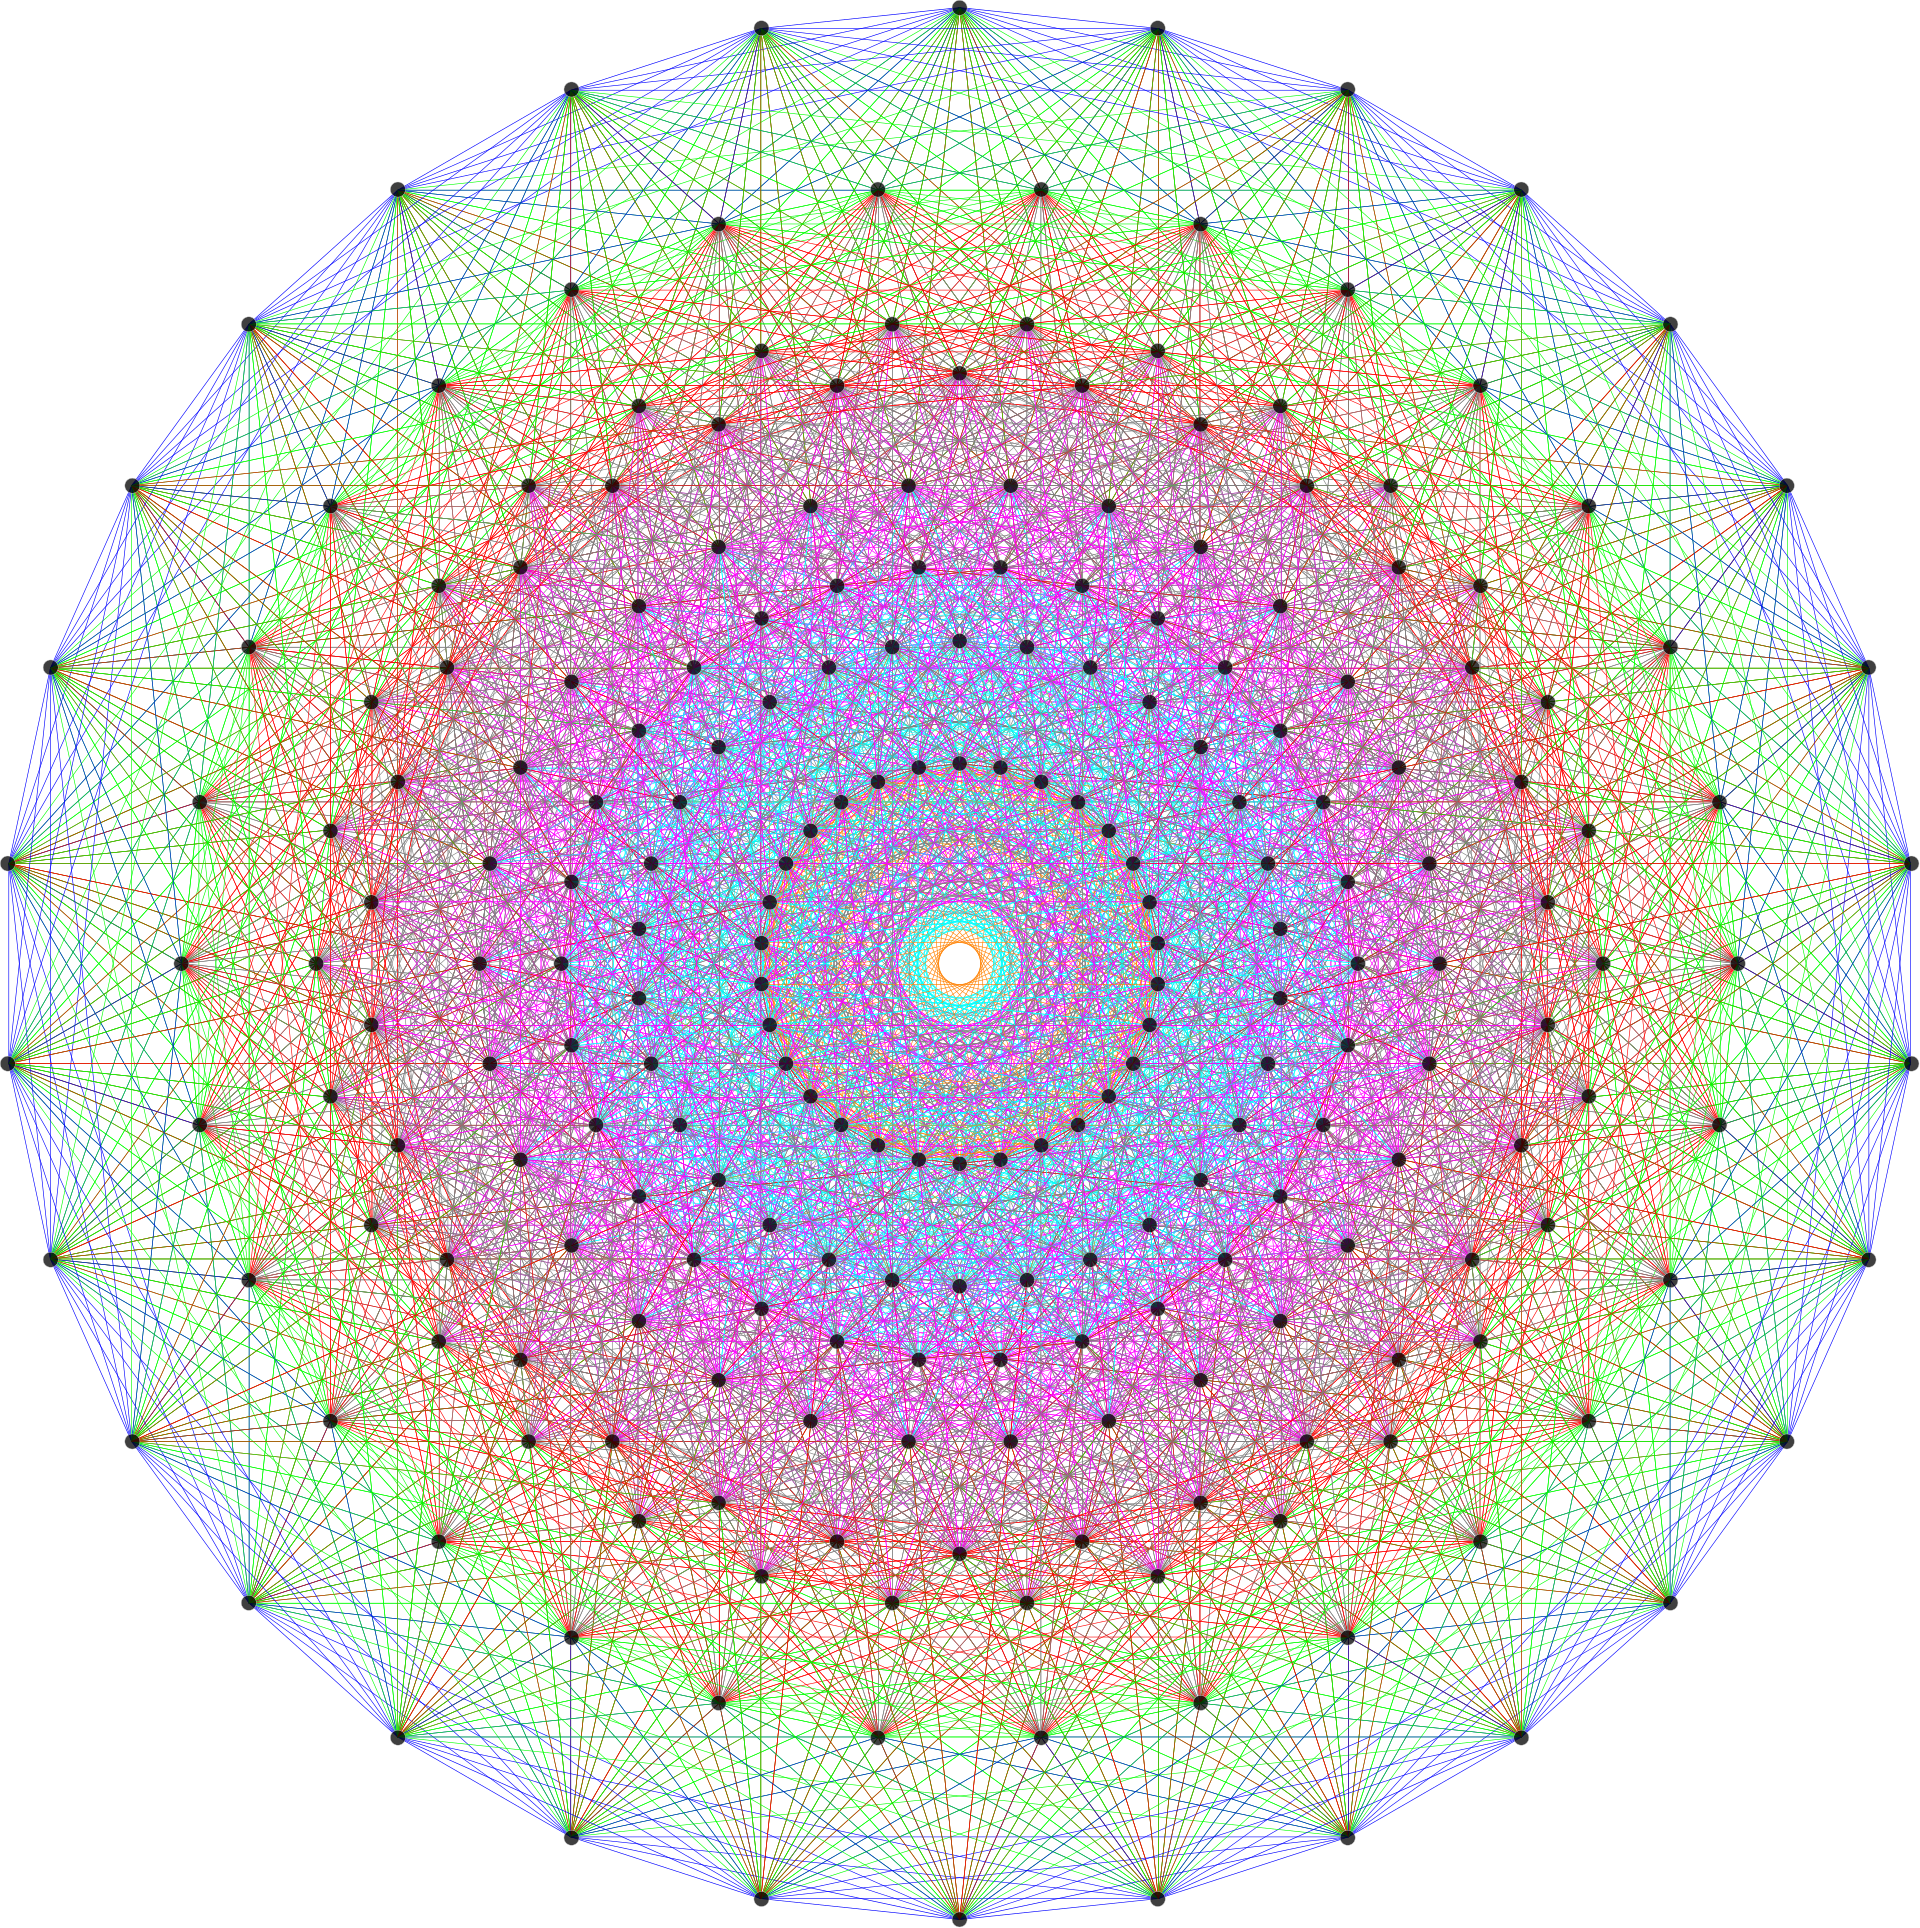
\includegraphics[scale=0.2]{cover}}
\date{}

\setlength{\abovedisplayskip}{10pt}
\setlength{\belowdisplayskip}{10pt}
\setlength{\abovedisplayshortskip}{5pt}
\setlength{\belowdisplayshortskip}{5pt}
\setlength\parindent{0pt}
\setlength{\jot}{5pt}

\maketitle
\tableofcontents

%\part{Fundamental Mathematics}
%
%\chapter{Axiomatic Set Theory}
%\input{chapters/1.axiomatic_set_theory}
%
%\chapter{Algebraic Structures}
%\section{Algebraic Structures}

\bd [Algebraic Structures]
A set $A$ (called the underlying set, carrier set or domain), together with a collection of maps (called operations) on $A$ of finite arity (typically binary operations), and a finite set of identities, known as axioms, that these operations must satisfy, is called an \textbf{algebraic structure}. Some algebraic structures also involve another set (called the scalar set).
\ed

Examples of algebraic structures with a single underlying set include groups,fields and rings. Examples of algebraic structures with two underlying sets include vector spaces, modules, and algebras. In this section we will review the most important algebraic structures for our purposes. \\

One has to be careful with the terminology since it changes depending on the area of mathematics. For example, in the context of universal algebra, the set $A$ with this structure is called an algebra, while, in other contexts, it is (somewhat ambiguously) called an algebraic structure, the term algebra being reserved for specific algebraic structures that are vector spaces over a field or modules over a commutative ring. \\

The properties of specific algebraic structures are studied in abstract algebra. The general theory of algebraic structures has been formalized in universal algebra. The language of category theory is used to express and study relationships between different classes of algebraic and non-algebraic objects. This is because it is sometimes possible to find strong connections between some classes of objects, sometimes of different kinds. For example, Galois theory establishes a connection between certain fields and groups: two algebraic structures of different kinds.

\section{Groups}

\bd [Group]
A \textbf{group}\index{field (algebraic)} is a tuple $(G,\cdot)$, where $G$ is a set (called the underlying set of the group) and $\cdot$ is a map (called operation) $G\times G \to G$ satisfying the following four group axioms:
\begin{itemize}
\item Closure: $\forall \, a,b \in G : a \cdot b \in G$;
\item Associativity: $\forall \, a,b,c \in G : (a \cdot b) \cdot c=a \cdot (b \cdot c)$;
\item Neutral Element: $\exists \, e \in G : \forall \, a \in G : a \cdot e = e \cdot a=a$;
\item Inverse Element: $\forall \, a \in G : \exists \, a^{-1} \in G : a \cdot a^{-1} =a^{-1}  \cdot a = e$;
\end{itemize}
\ed

The identity element $e$ of a group $G$ is often written as $1$ a notation inherited from the multiplicative identity. If a group is abelian, then one may choose to denote the group operation by $+$ and the identity element by $0$.\\

The result of the group operation may depend on the order of the operands. In other words, the result of combining element $a$ with element $b$ need not yield the same result as combining element $b$ with element $a$, so the equation $a \cdot b = b \cdot a$ may not be true for every two elements $a$ and $b$.

\bd [Abelian Group]
A group $G$ is called \textbf{Abelian} if on top of the four group axioms it also satisfies the axiom of commutativity:
\begin{itemize}
\item Commutativity: $\forall \, a,b \in G : a \cdot b = b \cdot a$;
\end{itemize}
\ed

Commutativity always holds in the group of integers under addition, because $a + b = b + a$ for any two integers (commutativity of addition). The symmetry group is an example of a group that is not abelian.

\section{Fields}

\bd [Field]
An \textbf{(algebraic) field}\index{field (algebraic)} is a triple $(K,+,\cdot)$, where $K$ is a set and $+,\cdot$ are maps $K\times K \to K$ satisfying the following axioms:
\begin{itemize}
\item $(K,+)$ is an abelian group, i.e.
\ben
\item[i)] Closure: $\forall \, a,b \in K : a + b \in K$;
\item[ii)] Associativity: $\forall \, a,b,c \in K : (a+b)+c=a+(b+c)$;
\item[iii)] Neutral Element: $\exists \, 0 \in K : \forall \, a \in K : a+0=0+a=a$;
\item[iv)] Inverse Element: $\forall \, a \in K : \exists \, {-a} \in K : a+(-a)=(-a)+a=0$;
\item[v)] Commutativity: $\forall \, a,b \in K : a+b=b+a$;
\een
\item $(K^*,\cdot)$, where $K^*:=K\sm\{0\}$, is an abelian group, i.e.
\ben
\item[vi)] Closure: $\forall \, a,b \in K^* : a \cdot b \in K^*$;
\item[vii)] Associativity: $\forall \, a,b,c \in K^* : (a\cdot b)\cdot c=a\cdot (b\cdot c)$;
\item[viii)] Neutral Element: $\exists \, 1 \in K^* : \forall \, a \in K^* : a\cdot 1=1\cdot a=a$;
\item[ix)] Inverse Element: $\forall \, a \in K^* : \exists \, a^{-1} \in K^* : a\cdot a^{-1}=a^{-1} \cdot a=1$;
\item[x)] Commutativity: $\forall \, a,b \in K^* : a\cdot b=b\cdot a$;
\een
\item the maps $+$ and $\cdot$ satisfy the distributive property:
\ben
\item[xi)] $\forall \, a,b,c \in K : (a+ b)\cdot c=a\cdot c + b\cdot c$;
\een
\end{itemize}
\ed

\br
In the above definition, we included axiom v for the sake of clarity, but in fact it can be proven starting from the other axioms.
\er

\section{Vector Spaces}

\bd [K-Vector Space]
Let $(K,+,\cdot)$ be a field. A $K$\textbf{-vector space}\index{vector space}, or \textbf{vector space over $K$} or \textbf{linear space over $K$} is a triple $(V,\oplus,\odot)$, where $V$ is a set and 
\bi{rl}
\oplus &\cl V\times V \to V\\
\odot  &\cl K\times V \to V
\ei
are maps satisfying the following axioms:
\begin{itemize}
\item $(V,\oplus)$ is an abelian group i.e.
\ben
\item[i)] Closure: $\forall \, v,w \in V : v \oplus w \in K$;
\item[ii)] Associativity: $\forall \, v,w,z \in V : (v \oplus w) \oplus z = v \oplus (w \oplus z)$;
\item[iii)] Neutral Element: $\exists \, 0 \in V : \forall \, v \in V : v \oplus 0 = 0 \oplus v = v$;
\item[iv)] Inverse Element: $\forall \, v \in V : \exists \, -v \in V : v \oplus (-v) = (-v) \oplus v = 0$;
\item[v)] Commutativity: $\forall \, v,w \in V : v \oplus w = w \oplus v$;
\een
\item the map $\odot$ is an \emph{action} of $K$ on $(V,\oplus)$:
\ben
\item[vi)] Distributivity Of Scalar Multiplication - Vector Addition: $\forall \, \lambda \in K : \forall \, v,w \in V : \lambda\odot(v\oplus w)=(\lambda\odot v)\oplus (\lambda\odot w)$;
\item[vii)] Distributivity Of Scalar Multiplication - Field Addition: $\forall \, \lambda,\mu \in K : \forall \, v \in V : (\lambda+\mu)\odot v= (\lambda \odot v) \oplus (\mu \odot v)$;
\item[viii)] Compatibility Of Scalar Multiplication - Field Multiplication $\forall \, \lambda,\mu \in K : \forall \, v \in V : (\lambda\cdot\mu)\odot v= \lambda \odot (\mu \odot v)$;
\item[ix)] Neutral Element Of Scalar Multiplication $\forall \, v \in V : 1\odot v = v$.
\een
\end{itemize}
\ed

The elements of a vector space are called \emph{vectors}, while the elements of $K$ are often called \emph{scalars}, and the map $\odot$ is called \emph{scalar multiplication}.

\subsection{Linear Maps}

As usual by now, we will look at the structure-preserving maps between vector spaces.

\bd [Linear Maps]
Let $(V,\oplus,\odot)$, $(W,\boxplus,\boxdot)$ be vector spaces over the same field $K$ and let $f\cl V\to W$ be a map. We say that $f$ is a \textbf{linear map}\index{linear map}\index{map!linear}, and we denote it as $f\cl V\xrightarrow{\sim}W$, if for all $v_1,v_2\in V$ and all $\lambda \in K$
\bse
f((\lambda\odot v_1)\oplus v_2) = (\lambda\boxdot f( v_1))\boxplus f(v_2).
\ese
\ed

From now on, we will drop the special notation for the vector space operations and suppress the dot for scalar multiplication. For instance, we will write the equation above as $f(\lambda v_1+v_2)=\lambda f(v_1)+f(v_2)$, hoping that this will not cause any confusion.

\bd [$\mathrm{Hom}(V,W)$]
Let $V$ and $W$ be vector spaces over the same field $K$. We define the set $\mathrm{Hom}(V,W)$ as the set of all linear maps between $V$ and $W$:
\bse
\mathrm{Hom}(V,W) := \{f \mid f\cl V\xrightarrow{\sim}W \}
\ese
\ed
$\mathrm{Hom}(V,W)$ can itself be made into a vector space over $K$ by defining:
\bi{rrCl}
\diamondplus \cl &\mathrm{Hom}(V,W) \times \mathrm{Hom}(V,W) &\to &\mathrm{Hom}(V,W)\\
& (f,g) & \mapsto & f \diamondplus g
\ei
where
\bi{rcCl}
f \diamondplus g \cl &V  &\xrightarrow{\sim} &W\\
& v & \mapsto & (f \diamondplus g)(v) := f(v)+g(v),
\ei 
and
\bi{rrCl}
\diamonddot \cl &K \times \mathrm{Hom}(V,W) &\to &\mathrm{Hom}(V,W)\\
& (\lambda,f) & \mapsto & \lambda \diamonddot f
\ei
where
\bi{rcCl}
\lambda \diamonddot f \cl &V  &\xrightarrow{\sim} &W\\
& v & \mapsto & (\lambda \diamonddot f)(v) := \lambda f(v).
\ei 
It is easy to check that both $f \diamondplus g$ and $\lambda \diamonddot f$ are indeed linear maps from $V$ to $W$. For instance, we have:
\bi{rCl"s}
(\lambda \diamonddot f)(\mu v_1+v_2) & = &  \lambda f(\mu v_1+v_2) & (by definition)\\
& = &  \lambda (\mu f( v_1)+f(v_2)) & (since $f$ is linear)\\
& = &  \lambda \mu f( v_1)+\lambda f(v_2) & (by axioms i and iii)\\
& = & \mu \lambda f( v_1)+\lambda f(v_2) & (since $K$ is a field)\\
& = & \mu (\lambda \diamonddot f)( v_1)+(\lambda \diamonddot f)(v_2) & 
\ei
so that $\lambda \diamonddot f\in \mathrm{Hom}(V,W)$. One should also check that $\diamondplus$ and $\diamonddot$ satisfy the vector space axioms.

\bd [Endomorphisms]
Let $V$ be a vector space. An \textbf{endomorphism}\index{endomorphism} of $V$ is a linear map $V\to V$. 
\ed

\bd [$\mathrm{End}(V)$]
Let $V$ be a vector space. We define the set $\mathrm{End}(V)$ as the set of all endomorphisms of $V$:  
\bse
\mathrm{End}(V):=\mathrm{Hom}(V,V)
\ese
\ed

\vspace{5pt}

It is easy to show that $\mathrm{End}(V)$ can again itself be made into a vector space over $K$.

\bd [Linear Isomorphism]
A bijective linear map is called a \textbf{linear isomorphism}\index{isomorphism!of vector spaces} of vector spaces.
\ed

\bd [Isomorphic Vector Spaces]
Two vector spaces are said to be \textbf{isomorphic} if there exists a linear isomorphism between them. We write $V\cong_\mathrm{vec}W$.
\ed

\bd [Automorphism]
Let $V$ be a vector space. An \textbf{automorphism}\index{automorphism} of $V$ is a linear isomorphism $V\to V$.
\ed

\bd [$\mathrm{Aut}(V)$]
Let $V$ be a vector space. We define the set $\mathrm{Aut}(V)$ as the set of all automorphisms of $V$:
\bse
\mathrm{Aut}(V):=\{f \in \mathrm{End}(V) \mid f \text{ is an isomorphism}\}
\ese
\ed

\br
Note that $\mathrm{Aut}(V)$ \textbf{cannot} be made into a vector space . It is however a group under the operation of composition of linear maps.
\er

\bd [Dual Vector Space]
Let $V$ be a vector space over $K$. The \textbf{dual}\index{vector space!dual}\index{dual space} vector space to $V$ is
\bse
V^*:=\Hom(V,K),
\ese
where $K$ is considered as a vector space over itself.
\ed

The dual vector space to $V$ is the vector space of linear maps from $V$ to the underlying field $K$, which are variously called \emph{linear functionals}, \emph{covectors}\index{covector}, or \emph{one-forms} on $V$. The dual plays a very important role, in that from a vector space and its dual, we will construct the tensor products.

\subsection{Basis Of Vector Spaces}

Given a vector space without any additional structure, the only notion of basis that we can define is a so-called Hamel basis.

\bd [Hamel Basis]
Let $(V,+,\cdot)$ be a vector space over $K$. A subset $\mathcal{B}\se V$ is called a \textbf{Hamel basis}\index{Hamel basis}\index{vector space!basis} for $V$ if 
\begin{itemize}
\item every finite subset $\{b_1,\ldots,b_N\}$ of $\mathcal{B}$ is linearly independent, i.e.\
\bse
\sum_{i=1}^N \lambda^ib_i = 0 \ \imp \ \lambda^1 = \cdots = \lambda^N = 0;
\ese
\item $\mathcal{B}$ is a \emph{generating} or \emph{spanning set} of $V$, i.e.\
\bse
\forall \, v \in V : \exists \, v^1,\ldots,v^M\in K : \exists \, b_1,\ldots,b_M \in \mathcal{B}:v=\ds \sum_{i=1}^Mv^ib_i.
\ese
\end{itemize}
\ed
\br
We can write the second condition more succinctly by defining
\bse
\lspan_K(\mathcal{B}) := \bigg\{\sum_{i=1}^n\lambda^ib_i \ \Big| \ \lambda^i\in K \land b_i\in \mathcal{B} \land n\geq 1\bigg\}
\ese
and thus writing $V = \lspan_K(\mathcal{B})$.
\er
\br
Note that we have been using superscripts for the elements of $K$, and these should not be confused with exponents.
\er
The following characterisation of a Hamel basis is often useful.
\bp
Let $V$ be a vector space and $\mathcal{B}$ a Hamel basis of $V$. Then $\mathcal{B}$ is a minimal spanning and maximal independent subset of $V$, i.e., if $S\se V$, then
\begin{itemize}
\item $\lspan(S) = V\ \Rightarrow \ |S| \geq |\mathcal{B}|$;
\item $S$ is linearly independent $\ \Rightarrow\ |S| \leq |\mathcal{B}|$. 
\end{itemize}
\ep

\bd [Dimension Of Vector Space]
Let $V$ be a vector space. The \textbf{dimension}\index{dimension!vector space}\index{vector space!dimension} of $V$ is $\dim V := |\mathcal{B}|$, where $\mathcal{B}$ is a Hamel basis for $V$.
\ed
Even though we will not prove it, it is the case that every Hamel basis for a given vector space has the same cardinality, and hence the notion of dimension is well-defined.

\bp
If $\dim V < \infty$ and $S\se V$, then we have the following:
\begin{itemize}
\item if $\lspan_K(S) = V$ and $|S| = \dim V$, then $S$ is a Hamel basis of $V$;
\item if $S$ is linearly independent and $|S| = \dim V$, then $S$ is a Hamel basis of $V$. 
\end{itemize}
\ep

\begin{theorem}
If $\dim V < \infty$, then $(V^*)^*\cong_\mathrm{vec}V$.
\end{theorem}

\br
Note that while we need the concept of basis to state this result (since we require $\dim V < \infty$), the isomorphism that we have constructed is independent of any choice of basis.
\er

\br
While a choice of basis often simplifies things, when defining new objects it is important to do so without making reference to a basis. If we do define something in terms of a basis (e.g.\ the dimension of a vector space), then we have to check that the thing is well-defined, i.e.\ it does not depend on which basis we choose.
\er

If $V$ is finite-dimensional, then $V^*$ is also finite-dimensional and $V\cong_\mathrm{vec}V^*$. Moreover, given a basis $\mathcal{B}$ of $V$, there is a spacial basis of $V^*$ associated to $\mathcal{B}$.

\bd [Dual Basis]
Let $V$ be a finite-dimensional vector space with basis $\mathcal{B}=\{e_1,\ldots,e_{\dim V}\}$. The \textbf{dual basis} to $\mathcal{B}$ is the unique basis $\mathcal{B'}=\{\epsilon^1,\ldots,\epsilon^{\dim V}\}$ of $V^*$ such that
\bse
\forall \, 1\leq i,j \leq \dim V :\quad  \epsilon^i(e_j) = \delta^i_j := \begin{cases}1 \quad \text{if }i=j\\0 \quad \text{if }i\neq j\end{cases}
\ese
\ed

\br
If $V$ is finite-dimensional, then $V$ is isomorphic to both $V^*$ and $(V^*)^*$. In the case of $V^*$, an isomorphism is given by sending each element of a basis $\mathcal{B}$ of $V$ to a different element of the dual basis $\mathcal{B}'$, and then extending linearly to $V$. You will (and probably already have) read that a vector space is \emph{canonically} isomorphic to its double dual, but \emph{not} canonically isomorphic to its dual, because an arbitrary choice of basis on $V$ is necessary in order to provide an isomorphism. 
\er

\subsection{Change Of Basis}

Let $V$ be a vector space over $K$ with $d=\dim V < \infty$ and let $\{e_1,\ldots,e_d\}$ be a basis of $V$. Consider a new basis $\{\widetilde e_1,\ldots,\widetilde e_d\}$. Since the elements of the new basis are also elements of $V$, we can expand them in terms of the old basis. We have:
\bse
\widetilde e_i = \sum_{j=1}^d A^j_{\phantom{j} i}\, e_j \qquad \text{for }1\leq i \leq d.
\ese
for some $A^j_{\phantom{j}i}\in K$. Similarly, we have
\bse
e_i = \sum_{j=1}^d B^j_{\phantom{j} i}\, \widetilde e_j \qquad \text{for }1\leq i \leq d.
\ese
for some $B^j_{\phantom{j}i}\in K$. It is a standard linear algebra result that the matrices $A$ and $B$, with entries $A^j_{\phantom{j}i}$ and $B^j_{\phantom{j}i}$ respectively, are invertible and, in fact, $A^{-1}=B$. \\

Once we have a basis $\mathcal{B}$, the expansion of $v\in V$ in terms of elements of $\mathcal{B}$ is, in fact, unique. Hence we can meaningfully speak of the \emph{components}\index{components} of $v$ in the basis $\mathcal{B}$. The notion of coordinates can also be generalised to the case of tensors that we will define next.

\subsection{Tensors}

\bd [Bilinear Maps]
Let $V$, $W$, $Z$ be vector spaces over $K$. A map $f\cl V\times W \to Z$ is said to be \textbf{bilinear}\index{bilinear map}\index{map!bilinear} if
\begin{itemize}
\item $\forall \, w\in W:\forall \, v_1,v_2\in V: \forall \,\lambda \in K : f(\lambda v_1+v_2,w)=\lambda f(v_1,w)+f(v_2,w)$;
\item $\forall \, v\in V:\forall \, w_1,w_2\in W: \forall \,\lambda \in K : f(v,\lambda w_1+w_2)=\lambda f(v,w_1)+f(v,w_2)$;
\end{itemize}
i.e.\ if the maps $v\mapsto f(v,w)$, for any fixed $w$, and $w\mapsto f(v,w)$, for any fixed $v$, are both linear as maps $V\to Z$ and $W\to Z$, respectively.
\ed

\br
Compare this with the definition of a linear map $f\cl V\times W \xrightarrow{\sim} Z$:
\bse
\forall \, x,y\in V \times W : \forall \, \lambda \in K : f(\lambda x+y)=\lambda f(x)+f(y).
\ese
More explicitly, if $x=(v_1,w_1)$ and $y = (v_2,w_2)$, then:
\bse
f(\lambda (v_1,w_1)+(v_2,w_2))=\lambda f((v_1,w_1))+f((v_2,w_2)).
\ese
A bilinear map out of $V\times W$ is \emph{not} the same as a linear map out of $V\times W$. In fact, bilinearity is just a special kind of non-linearity.
\er

\be
The map $f\cl \R^2\to \R$ given by $(x,y)\mapsto x+y$ is linear but not bilinear, while the map $(x,y)\mapsto xy$ is bilinear but not linear.
\ee

We can immediately generalise the above to define \emph{multilinear} maps out of a Cartesian product of vector spaces.

\bd [Tensors]
Let $V$ be a vector space over $K$. A \textbf{$(p,q)$-tensor}\index{tensor} $T$ on $V$ is a multilinear map
\bse
T\cl \underbrace{V^*\times\cdots \times V^*}_{p \text{ copies}} \times \underbrace{V \times \cdots \times V}_{q \text{ copies}} \to K.
\ese
\ed

\br
By convention, a $(0,0)$ on $V$ is just an element of $K$, and hence $T^0_0V=K$.
\er

\bd [Covariant / Contravariant Tensor]
A type $(p,0)$ tensor is called a \textbf{covariant $p$-tensor}, while a tensor of type $(0,q)$ is called a \textbf{contravariant $q$-tensor}.
\ed

\bd [$T^p_q V$]
We define the set of all $(p,q)$-tensors $T$ as:
\bse
T^p_q V\index{$T^p_qV$} := \underbrace{V\otimes\cdots \otimes V}_{p \text{ copies}} \otimes \underbrace{V^* \otimes \cdots \otimes V^*}_{q \text{ copies}} := \{T\mid T \text{ is a $(p,q)$-tensor on }V\}. 
\ese
\ed

\br
Note that to define $T^p_q V$ as a set, we should be careful and invoke the principle of restricted comprehension, i.e.\ we should say where the $T$s are coming from. In general, say we want to build a set of maps $f\cl A\to B$ satisfying some property $p$. Recall that the notation $f\cl A \to B$ is hiding the fact that is a relation (indeed, a functional relation), and a relation between $A$ and $B$ is a subset of $A\times B$. Therefore, we ought to write:
\bse
\{f\in \cP(A\times B)\mid f\cl A\to B \text{ and } p(f)\}.
\ese
In the case of $T^p_q V$ we have:
\bse
T^p_q V := \big\{T \in \cP\bigl(\underbrace{V^*\times\cdots \times V^*}_{p \text{ copies}} \times \underbrace{V \times \cdots \times V}_{q \text{ copies}} \times K\bigr) \mid  T \text{ is a $(p,q)$-tensor on }V\big\},
\ese
although we will not write this down every time.
\er

The set $T^p_q V$ can be equipped with a $K$-vector space structure by defining
\bi{rrCl}
\oplus\cl &T^p_q V \times T^p_q V &\to &T^p_q V\\
& (T,S) & \mapsto & T \oplus S
\ei
and
\bi{rrCl}
\odot \cl &K \times T^p_q V &\to &T^p_q V\\
& (\lambda,T) & \mapsto & \lambda \odot T,
\ei
where $T \oplus S$ and $\lambda \odot T$ are defined pointwise, as we did with $\mathrm{Hom}(V,W)$. \\

We now define an important way of obtaining a new tensor from two given ones.

\bd [Tensor Product]
Let $T\in T^p_q V$ and $S\in T^r_s V$. The \textbf{tensor product}\index{tensor!product} of $T$ and $S$ is the tensor $T\otimes S\in T^{p+r}_{q+s}V$ defined by:
\bi{rl}
(T\otimes S)(\omega_1,\ldots,\omega_p,\omega_{p+1},\ldots,\omega_{p+r},v_1,&\ldots,v_q,v_{q+1},\ldots,v_{q+s})\\
:=T(\omega_1,\ldots,\omega_p,v_1,&\ldots,v_q)\,S(\omega_{p+1},\ldots,\omega_{p+r},v_{q+1},\ldots,v_{q+s}),
\ei
with $\omega_i\in V^*$ and $v_i\in V$.
\ed

Some examples are in order.

\be
\ben[label=\alph*)]
\item $T^0_1 V := \{T\mid T\cl V \xrightarrow{\sim} K\} = \mathrm{Hom}(V,K) =: V^*$. Note that here multilinear is the same as linear since the maps only have one argument.
\item $T^1_1V\equiv V\otimes V^*:=\{T\mid T\text{ is a bilinear map }V^*\times V \to K\}$. We claim that this is the same as $\mathrm{End}(V^*)$. Indeed, given $T\in  V\otimes V^*$, we can construct $\widehat T \in \mathrm{End}(V^*)$ as follows:
\bi{rrCl}
\widehat T \cl &V^* &\xrightarrow{\sim}& V^*\\
& \omega & \mapsto & T(-,\omega)
\ei
where, for any fixed $\omega$, we have
\bi{rrCl}
T (-,\omega) \cl &V &\xrightarrow{\sim}& K\\
& v & \mapsto & T(v,\omega).
\ei
The linearity of both $\widehat T$ and $T(-,\omega)$ follows immediately from the bilinearity of $T$. Hence $T(-,\omega)\in V^*$ for all $\omega$, and $\widehat T \in \mathrm{End}(V^*)$. This correspondence is invertible, since can reconstruct $T$ from $\widehat T$ by defining
\bi{rrCl}
T  \cl &V \times V^* &\to & K\\
& (v,\omega) & \mapsto & T(v,\omega):=(\widehat T(\omega))(v).
\ei
The correspondence is in fact linear, hence an isomorphism, and thus \bse
T^1_1V\cong_\mathrm{vec}\mathrm{End}(V^*).
\ese
\een

Other examples we would like to consider are
\ben[label=\alph*),start=3]
\item $T^0_1 V \stackrel{?}{\cong}_\mathrm{vec} V$: while you will find this stated as true in some physics textbooks, it is in fact \emph{not true} in general;
\item $T^1_1 V \stackrel{?}{\cong}_\mathrm{vec} \mathrm{End}(V)$: This is also not true in general;
\item $(V^*)^* \stackrel{?}{\cong}_\mathrm{vec} V$: This only holds if $V$ is finite-dimensional.
\een
\ee

\bd [Components Of A Tensor]
Let $V$ be a finite-dimensional vector space over $K$ with basis $\mathcal{B}=\{e_1,\ldots,e_{\dim V}\}$ and dual basis $\{\epsilon^1,\ldots,\epsilon^{\dim V}\}$ and let $T\in T^p_qV$. We define the \textbf{components}\index{tensor!components} of $T$ in the basis $\mathcal{B}$ to be the numbers
\bse
T^{a_1\ldots a_p}_{\phantom{a_1\ldots a_p}b_1\ldots b_q} := T(\epsilon^{a_1},\ldots,\epsilon^{a_p},e_{b_1},\ldots,e_{b_q})\in K,
\ese
where $1\leq a_i,b_j\leq \dim V$.
\ed

Just as with vectors, the components completely determine the tensor. Indeed, we can reconstruct the tensor from its components by using the basis:
\bse
T = \underbrace{\sum_{a_1=1}^{\dim V}\!\cdots\!\sum_{b_q=1}^{\dim V}}_{p+q \text{ sums}} T^{a_1\ldots a_p}_{\phantom{a_1\ldots a_p}b_1\ldots b_q} e_{a_1}\otimes\cdots\otimes e_{a_p} \otimes \epsilon^{b_1}\otimes \cdots\otimes \epsilon^{b_q},
\ese
where the $e_{a_i}$s are understood as elements of $T^1_0V\cong_\mathrm{vec}V$ and the $\epsilon^{b_i}s$ as elements of $T^0_1V\cong_\mathrm{vec}V^*$. Note that each summand is a $(p,q)$-tensor and the (implicit) multiplication between the components and the tensor product is the scalar multiplication in $T^p_q V$.

\subsection{Notational Conventions}
From now on, we will employ the Einstein's summation convention, which consists in suppressing the summation sign when the indices to be summed over each appear once as a subscript and once as a superscript in the same term. For example, we write
\bi{rcl}
v=v^ie_i \qquad &\text{and}& \qquad T=T^{ij}_{\phantom{ij}k}e_i\otimes e_j \otimes f^k
\ei
instead of
\bi{rcl}
v=\sum_{i=1}^dv^ie_i \qquad &\text{and}& \qquad T=\sum_{i=1}^d\sum_{j=1}^d\sum_{k=1}^d
T^{ij}_{\phantom{ij}k}e_i\otimes e_j \otimes f^k.
\ei

Indices that are summed over are called \emph{dummy indices}; they always appear in pairs and clearly it doesn't matter which particular letter we choose to denote them, provided it doesn't already appear in the expression. Indices that are not summed over are called \emph{free indices}; expressions containing free indices represent multiple expressions, one for each value of the free indices; free indices must match on both sides of an equation. The ranges over which the indices run are usually understood and not written out. \\

The convention on which indices go upstairs and which downstairs (which we have already been using) is that:
\begin{itemize}
\item the basis vectors of $V$ carry downstairs indices;
\item the basis vectors of $V^*$ carry upstairs indices;
\item all other placements are enforced by the Einstein's summation convention.
\end{itemize}
For example, since the components of a vector must multiply the basis vectors and be summed over, the Einstein's summation convention requires that they carry upstair indices.

\be
Using the summation convention, we have:
\ben[label=\alph*)]
\item $\epsilon^a(v) = \epsilon^a(v^be_b)=v^b\epsilon^a(e_b)=v^b\delta^a_b=v^a$;
\item $\omega(e_b)=(\omega_a\epsilon^a)(e_b)=\omega_a\epsilon^a(e_b)=\omega_b$;
\item $\omega(v)=\omega_a\epsilon^a(v^be_b)=\omega_av^a$;
\een
where $v\in V$, $\omega \in V^*$, $\{e_i\}$ is a basis of $V$ and $\{\epsilon^j\}$ is the dual basis to $\{e_i\}$.
\ee

\br
The Einstein's summation convention should only be used when dealing with linear spaces and multilinear maps. The reason for this is the following. Consider a map $\phi\cl V\times W \to Z$, and let $v=v^ie_i\in V$ and $w=w^i\widetilde e_i\in W$. Then we have:
\bse
\phi(v,w) = \phi\,\bigg({\color{lightgray}\sum_{i=1}^d}v^ie_i,{\color{lightgray}\sum_{j=1}^{\widetilde{d}}} w^j\widetilde e_j\bigg) = {\color{lightgray}\sum_{i=1}^d \sum_{j=1}^{\widetilde{d}}}\phi(v^ie_i,w^j\widetilde e_j)= {\color{lightgray}\sum_{i=1}^d \sum_{j=1}^{\widetilde{d}}}v^iw^j\phi(e_i,\widetilde e_j).
\ese
Note that by suppressing the greyed out summation signs, the second and third term above are indistinguishable. But this is only true if $\phi$ is bilinear! Hence the summation convention should not be used (at least, not without extra care) in other areas of mathematics.
\er

\br
Having chosen a basis for $V$ and the dual basis for $V^*$, it is very tempting to think of $v=v^ie_i\in V$ and $\omega=\omega_i\epsilon^i\in V^*$ as $d$-tuples of numbers. In order to distinguish them, one may choose to write vectors as \emph{columns} of numbers and covectors as \emph{rows} of numbers:
\bse
v =v^ie_i \quad \leftrightsquigarrow\quad v\ \hat{=} \left(
\ba{c}
v^1\\
\vdots\\
v^d
\ea
\right)
\ese
and
\bse
\omega =\omega_i\epsilon^i \quad \leftrightsquigarrow\quad \omega \ \hat{=} \ (\omega_1,\ldots,\omega_d).
\ese

\vspace{5pt}

Given $\phi\in\mathrm{End}(V)\cong_\mathrm{vec}T^1_1V$, recall that we can write $\phi = \phi^i_{\phantom{i}j}\, e_i\otimes \epsilon^j$, where $\phi^i_{\phantom{i}j}:=\phi(\epsilon^i,e_j)$ are the components of $\phi$ with respect to the chosen basis. It is then also very tempting to think of $\phi$ as a square array of numbers:
\bse
\phi = \phi^i_{\phantom{i}j}\, e_i\otimes \epsilon^j \quad \leftrightsquigarrow\quad \phi \ \hat{=} \left(
\ba{cccc}
\phi^1_{\phantom{1}1} & \phi^1_{\phantom{1}2} & \cdots & \phi^1_{\phantom{1}d}\\
\phi^2_{\phantom{2}1} & \phi^2_{\phantom{2}2} & \cdots & \phi^2_{\phantom{2}d}\\
\vdots & \vdots & \ddots & \vdots\\
\phi^d_{\phantom{d}1} & \phi^d_{\phantom{d}2} & \cdots & \phi^d_{\phantom{d}d} 
\ea
\right)
\ese

\vspace{5pt}

The convention here is to think of the $i$ index on $\phi^i_{\phantom{i}j}$ as a \emph{row index}, and of $j$ as a \emph{column index}.
\er

We cannot stress enough that this is pure convention. Its usefulness stems from the following example.

\be
If $\dim V<\infty$, then we have $\mathrm{End}(V)\cong_\mathrm{vec}T^1_1V$. Explicitly, if $\phi \in \mathrm{End}(V)$, we can think of $\phi \in T^1_1V$, using the same symbol, as
\bse
\phi(\omega,v):=\omega(\phi(v)).
\ese
Hence the components of $\phi\in\mathrm{End}(V)$ are $\phi^a_{\phantom{a}b}:=\epsilon^a(\phi(e_b))$. \\

Now consider $\phi,\psi\in\mathrm{End}(V)$. Let us determine the components of $\phi\circ \psi$. We have:
\bi{rCl}
(\phi\circ \psi)^a_{\phantom{a}b} &:=& (\phi\circ \psi)(\epsilon^a,e_b)\\
&:=&\epsilon^a( (\phi\circ \psi)(e_b))\\
&=& \epsilon^a( (\phi(\psi(e_b)))\\
&=& \epsilon^a(\phi(\psi^m_{\phantom{m}b}\,e_m))\\
&=& \psi^m_{\phantom{m}b} \epsilon^a( \phi(e_m))\\
&:=& \psi^m_{\phantom{m}b}\, \phi^a_{\phantom{a}m} .
\ei
The multiplication in the last line is the multiplication in the field $K$, and since that's commutative, we have $\psi^m_{\phantom{m}b}\, \phi^a_{\phantom{a}m}  = \phi^a_{\phantom{a}m} \, \psi^m_{\phantom{m}b}$. However, in light of the convention introduced in the previous remark, the latter is preferable. Indeed, if we think of the superscripts as row indices and of the subscripts as column indices, then $\phi^a_{\phantom{a}m} \, \psi^m_{\phantom{m}b}$ is the entry in row $a$, column $b$, of the matrix product $\phi\psi$. \\

Similarly, $\omega(v)=\omega_mv^m$ can be thought of as the \emph{dot product} $\omega \cdot v\equiv\omega^Tv$, and
\bse
\phi(v,w)=w_a\,\phi^a_{\phantom{a}b}\,v^b \quad   \leftrightsquigarrow\quad \omega^T\phi v.
\ese
The last expression is could mislead you into thinking that the transpose is a ``good'' notion, but in fact it is not. It is very bad notation. It almost pretends to be basis independent, but it is not at all. \\

The moral of the story is that you should try your best \emph{not} to think of vectors, covectors and tensors as arrays of numbers. Instead, always try to understand them from the abstract, intrinsic, component-free point of view.
\ee

As a final note in the notational conventions let's see the change of components under a change of basis using the new notation.\\

Recall that if $\{e_a\}$ and $\{\widetilde e_a\}$ are basis of $V$, we have
\bse
\widetilde e_a=A^b_{\phantom{b}a}e_b \qquad \text{and}  \qquad e_a=B^m_{\phantom{m}a}\widetilde e_m,
\ese
with $A^{-1}=B$. Note that in index notation, the equation $AB=I$ reads $A^a_{\phantom{a}m}B^m_{\phantom{m}b}=\delta^a_b$. \\

We now investigate how the components of vectors and covectors change under a change of basis. 
\ben[label=\alph*)]
\item Let $v=v^ae_a=\widetilde v^a\widetilde e_a\in V$. Then:
\bse
v^a = \epsilon^a(v) = \epsilon^a(\widetilde v^b\widetilde e_b) = \widetilde v^b
\epsilon^a(\widetilde e_b) = \widetilde v^b \epsilon^a(A^m_{\phantom{m}b}e_m) = A^m_{\phantom{m}b} \widetilde v^b\epsilon^a(e_m)=A^a_{\phantom{a}b} \widetilde v^b.
\ese
\item Let $\omega = \omega_a\epsilon^a = \widetilde \omega_a\widetilde \epsilon^a  \in V^*$. Then:
\bse
\omega_a := \omega(e_a) = \omega(B^m_{\phantom{m}a}\widetilde e_m) = B^m_{\phantom{m}a}\omega(\widetilde e_m) = B^m_{\phantom{m}a}\widetilde \omega_m .
\ese
\een
Summarising, for $v\in V$, $\omega \in V^*$ and $\widetilde e_a=A^b_{\phantom{b}a}e_b$, we have:
\bi{rClcrCl}
v^a & = & A^a_{\phantom{a}b} \widetilde v^b &\qquad & \omega_a &= & B^b_{\phantom{b}a}\widetilde \omega_b \\
\widetilde v^a & = & B^a_{\phantom{a}b}  v^b & & \widetilde \omega_a &= & A^b_{\phantom{b}a}\omega_b 
\ei
The result for tensors is a combination of the above, depending on the type of tensor.
\ben
\item[c)] Let $T\in T^p_qV$. Then:
\bse
T^{a_1\ldots a_p}_{\phantom{a_1\ldots a_p}b_1\ldots b_q} = A^{a_1}_{\phantom{a_1}m_1}\cdots A^{a_p}_{\phantom{a_p}m_p} B^{n_1}_{\phantom{n_1}b_1} \cdots B^{n_q}_{\phantom{n_q}b_q} \widetilde T^{m_1\ldots m_p}_{\phantom{m_1\ldots m_p}n_1\ldots n_q},
\ese
i.e.\ the upstair indices transform like vector indices, and the downstair indices transform like covector indices. 
\een

\section{Rings}

\bd [Ring]
A \textbf{ring}\index{ring} is a triple $(R,+,\cdot)$, where $R$ is a set and $+,\cdot\cl R\times R\to R$ are maps satisfying the following axioms
\begin{itemize}
\item $(R,+)$ is an abelian group:
\ben
\item[i)] Closure: $\forall \, a,b \in R : a + b \in R$;
\item[ii)] Associativity: $\forall \, a,b,c \in R : (a+b)+c=a+(b+c)$;
\item[iii)] Neutral Element: $\exists \, 0 \in R : \forall \, a \in R : a+0=0+a=a$;
\item[iv)] Inverse Element: $\forall \, a \in R : \exists \, {-a} \in R : a+(-a)=(-a)+a=0$;
\item[v)] Commutativity: $\forall \, a,b \in R : a+b=b+a$;
\een
\item the operation $\cdot$ is closed and associative in $R^*:=R\sm\{0\}$:
\ben
\item[vi)] Closure: $\forall \, a,b \in R^* : a \cdot b \in R^*$;
\item[vii)] Associativity: $\forall \, a,b,c \in R^* : (a\cdot b)\cdot c=a\cdot (b\cdot c)$;
\een
\item the maps $+$ and $\cdot$ satisfy the distributive properties:
\ben
\item[viii)] $\forall \, a,b,c \in R : (a+ b)\cdot c=a\cdot c + b\cdot c$;
\item[ix)] $\forall \, a,b,c \in R : a \cdot (b+c)=a\cdot b + a\cdot c$.
\een
\end{itemize}

Note that since $\cdot$ is not required to be commutative, axioms viii and ix are both necessary. In the case of fields where $\cdot$ was commutative, ix followed from viii and commutativity of $\cdot$.
\ed

\bd [Commutative / Unital / Division Rings]
A ring $(R,+,\cdot)$ is said to be
\begin{itemize}
\item \textbf{commutative} if $\ \forall \, a,b\in R : a\cdot b = b \cdot a$;
\item \textbf{unital} if $\ \exists\, 1\in R : \forall \, a\in R : 1\cdot a = a \cdot 1 = a$;
\item a \textbf{division} (or \textbf{skew}) \emph{ring} if it is unital and 
\bse
\forall\, a \in R\sm\{0\} : \exists \, a^{-1}\in R\sm\{0\}: \ a\cdot a^{-1}=a^{-1}\cdot a = 1.
\ese
\end{itemize}
\ed

In a unital ring, an element for which there exists a multiplicative inverse is said to be a \emph{unit}. The set of units of a ring $R$ is denoted by $R^*$ (not to be confused with the vector space dual) and forms a group under multiplication. Then, $R$ is a division ring iff $R^*=R\sm\{0\}$.

\be
The sets $\Z$, $\Q$, $\R$, and $\C$ are all rings under the usual operations. They are also all fields, except $\Z$.
\ee

In general, if $(A,+,\cdot,\bullet)$ is an algebra, then $(A,+,\bullet)$ is a ring.

\section{Modules}

\bd [$R$-Module]
Let $(R,+,\cdot)$ be a unital ring. An \textbf{$R$-module}\index{module} is a triple $(M,\oplus,\odot)$ where $M$ is a set and
\bi{rrCl}
\oplus \cl & M \times M & \to & M\\
\odot \cl & R \times M & \to & M
\ei
are maps satisfying the following axioms:
\begin{itemize}
\item $(M,\oplus)$ is an abelian group i.e
\ben
\item[i)] Closure: $\forall \, m,n \in M : m \oplus n \in M$;
\item[ii)] Associativity: $\forall \, m,n,s \in M : (m \oplus n) \oplus s = m \oplus (n \oplus s)$;
\item[iii)] Neutral Element: $\exists \, 0 \in M : \forall \, m \in M : m \oplus 0 = 0 \oplus m = m$;
\item[iv)] Inverse Element: $\forall \, m \in M : \exists \, -m \in M : m \oplus (-m) = (-m) \oplus m = 0$;
\item[v)] Commutativity: $\forall \, m,n \in M : m \oplus n = n \oplus m$;
\een
\item the map $\odot$ is an \emph{action} of $R$ on $(M,\oplus)$:
\ben
\item[vi)] Distributivity Of Scalar Multiplication - Vector Addition: $\forall \, r \in R : \forall \, m,n \in M : r \odot (m\oplus n) = (r \odot m) \oplus (r \odot n)$;
\item[vii)] Distributivity Of Scalar Multiplication - Field Addition: $\forall \, r,s \in K : \forall \, m \in V : (r+s)\odot m = (r\odot m)\oplus (s\odot m)$;
\item[viii)] Compatibility Of Scalar Multiplication - Field Multiplication $\forall \, r,s \in R : \forall \, m \in M : (r\cdot s)\odot m = r \odot (s\odot m)$;
\item[ix)] Neutral Element Of Scalar Multiplication $\forall \, m \in M : 1\odot m = m$.
\een
\end{itemize}
\ed

So, modules are simply vector spaces over rings instead of fields. For this reason, most definitions we had for vector spaces carry over unaltered to modules.

\be
Any ring $R$ is trivially a module over itself, in the sense that every field $K$ is a vector space over itself.
\ee

In the following, we will usually denote $\oplus$ by $+$ and suppress the $\odot$, as we did with vector spaces.\\

\bd [Direct Sum Of Modules]
The \textbf{direct sum} of two $R$-modules $M$ and $N$ is the $R$-module $M\oplus N$, which has $M\times N$ as its underlying set and operations (inherited from $M$ and $N$) defined component-wise. 
\ed

Note that while we have been using $\oplus$ to temporarily distinguish two ``plus-like'' operations in different spaces, the symbol $\oplus$ is the standard notation for the direct sum.

\bd [Finitely Generated / Free / Projective Modules]
An $R$-module $M$ is said to be
\begin{itemize}
\item \textbf{finitely generated} if it has a finite generating set;
\item \textbf{free} is it has a basis;
\item \textbf{projective} if it is a direct summand of a free $R$-module $F$, i.e.\
\bse
M \oplus Q = F
\ese
for some $R$-module $Q$.
\end{itemize}
\ed

\be
Clearly, every free module is also projective.
\ee

\bd [R-Linear Maps]
Let $M$ and $N$ be two $R$-modules. A map $f\cl M \to N$ is said to be an \textbf{$R$-linear map}, or an \textbf{$R$-module homomorphism}, if
\bse
\forall \, r\in R : \forall \, m_1,m_2\in M : \ f(rm_1 + m_2)=rf(m_1)+f(m_2),
\ese
where it should be clear which operations are in $M$ and which in $N$.
\ed

\bd [Module Isomorphisms]
A bijective module homomorphism is said to be a \textbf{module isomorphism}\index{isomorphism!of modules}.
\ed

\bd [Isomorphic Modules]
Two modulesare said to be \textbf{isomorphic} if there exists a module isomorphism between them. We write $M\cong_{\mathrm{mod}}N$.
\ed

\bp
If a finitely generated module $R$-module $F$ is free, and $d\in \N$ is the cardinality of a finite basis, then
\bse
F\cong_\mathrm{mod} = \underbrace{R\oplus\cdots\oplus R}_{d \text{ copies}} =: R^d.
\ese
\ep
One can show that if $R^d\cong_\mathrm{mod} R^{d'}$, then $d=d'$ and hence, the concept of dimension is well-defined for finitely generated, free modules.

\begin{theorem}
Let $P,Q$ be finitely generated (projective) modules over a commutative ring $R$. Then
\bse
\Hom_R(P,Q) := \{\phi\cl P \xrightarrow{\sim} Q \mid \phi \text{ \normalfont is $R$-linear}\}
\ese
is again a finitely generated (projective) $R$-module, with operations defined pointwise.
\end{theorem}

The proof is exactly the same as with vector spaces. As an example, we can use this to define the dual of a module.

\subsection{Basis Of Modules}

The key fact that sets modules apart from vector spaces is that, unlike a vector space, an $R$-module need not have a basis, unless $R$ is a division ring. This is actually a well-known theorem that we will state but not prove.

\begin{theorem}
\label{thm:everybasis}
If $D$ is a division ring, then any $D$-module $V$ admits a basis.
\end{theorem}

\bc
Every vector space has a basis, since any field is also a division ring.
\ec

\section{Algebras}

\bd [Algebra]
Let $K$ be a field, and let $A$ be a vector space over $K$ equipped with an additional bilinear map (called binary operation or product) $\bullet \cl A\times A \to A$. The quadruple $(A,+,\cdot,\bullet)$ is called an \textbf{algebra}\index{algebra} over a field $K$.
\ed

\bd [Associative / Unital / Commutative Algebra]
An algebra $(A,+,\cdot,\bullet)$ is said to be
\ben[label=\roman*)]
\item \textbf{Associative} if $\ \forall \, v,w,z\in A :  v\bullet (w\bullet z) = (v\bullet w)\bullet z$;
\item \textbf{Unital} if $\ \exists \, \mathbf{1} \in A : \forall \, v \in V : \mathbf{1}\bullet v = v \bullet \mathbf{1} = v$;
\item \textbf{Commutative} or \emph{abelian} if $\ \forall \, v,w\in A :  v\bullet w = w\bullet v$.
\een
\ed

\bd [Derivation]
Let $A$ and $B$ be algebras. A \textbf{derivation}\index{derivation} on $A$ is a linear map $D\cl A \xrightarrow{\sim}B$ satisfying the Leibniz rule
\bse
D(v\bullet_Aw)= D(v)\bullet_Bw +_B v \bullet_B D(w).
\ese
for all $v,w \in A$.
\ed

\section{Lie Algebras}

An important class of algebras, that we will also see later, are the so-called Lie algebras, in which the product $v\bullet w$ is denoted as $[v,w]$ called the ``commutator" or ``Lie bracket".  Let's first define it, and then use it to define the corresponding Lie algebra.

\bd [Lie Bracket]
Let $K$ be a field, $A$ be a vector space over $K$ and $v,w \in A$. The \textbf{Lie bracket}\index{Lie bracket} (or \textbf{commutator}) of $v$ and $w$ defined as
\bi{rrCl}
[v,w] \cl & A \times A & \to & A\\ 
& (v,w) & \mapsto & [v,w] :=v w  - w v
\ei
\ed

\bd [Lie Algebra]
A \textbf{Lie algebra}\index{Lie algebra} $A$ is an algebra whose product $[-,-]$, called \emph{Lie bracket}\index{Lie bracket}, satisfies
\ben[label=\roman*)]
\item bilinearity: $A \times A \to A$
\item antisymmetry: $\ \forall\, v\in A : [v,v]=0$;
\item the Jacobi identity\index{Jacobi identity}: $\ \forall\, v,w,z\in A : [v,[w,z]] + [w,[z,v]] + [z,[v,w]] = 0$.
\een
Note that the zeros above represent the additive identity element in $A$, not the zero scalar
\ed

The antisymmetry condition immediately implies $[v,w]=-[w,v]$ for all $v,w\in A$, hence a (non-trivial) Lie algebra cannot be unital.

\be
Let $V$ be a vector space over $K$. Then $(\End(V),+,\cdot,\circ)$ (where the product is simply the composition of endomorphisms) is an associative, unital, non-commutative algebra over $K$. Define:
\bi{rrCl}
[-,-] \cl &\End(V)\times \End(V) &\to& \End(V)\\
&(\phi,\psi) &\mapsto& [\phi,\psi] := \phi\circ\psi-\psi\circ\phi.
\ei
It is instructive to check that $(\End(V),+,\cdot,[-,-])$ is a Lie algebra over $K$. In this case, the Lie bracket is typically called the \emph{commutator}\index{commutator}.
\ee

In general, given an associative algebra $(A,+,\cdot,\bullet)$, if we define 
\bse
[v,w]:=v\bullet w-w\bullet v,
\ese
then $(A,+,\cdot,[-,-])$ is a Lie algebra.

\be
Consider again the Lie algebra $(\End(V),+,\cdot,[-,-])$ and fix $\xi \in \End(V)$. If we define
\bi{rrCl}
D_\xi := [\xi,-] \cl &\End(V) &\xrightarrow{\sim} &\End(V)\\
& \phi & \mapsto & [\xi,\phi],
\ei
then $D_\xi$ is a derivation on $(\End(V),+,\cdot,[-,-])$ since it is linear and
\bi{rCl"s}
D_\xi([\phi,\psi]) & := & [\xi,[\phi,\psi]]\\
& = & -[\psi,[\xi,\phi]] -[\phi,[\psi,\xi]]& (by the Jacobi identity)\\
& = & [[\xi,\phi],\psi]+[\phi,[\xi,\psi]] & (by antisymmetry)\\
& =: &  [D_\xi(\phi),\psi]+[\phi,D_\xi(\psi)].
\ei
This construction works in general Lie algebras as well.
\ee

Of course one can construct an algebra over a ring, by imposing all the axioms on a module instead of a vector space. Same definitions apply for an algebra over a ring with the appropriate changes when needed.

\subsection{Classification Of Lie Algebras}

One of the most important topics on Lie algebras is the classification of them. While it is possible to classify Lie algebras more generally, we will only consider the classification of finite-dimensional complex Lie algebras, i.e.\ Lie algebras $(L,[-,-])$ where $L$ is a finite-dimensional $\C$-vector space. 

If $A,B$ are Lie subalgebras of a Lie algebra $(L,[-,-])$ over $K$, then
\bse
[A,B] := \lspan_K\bigl(\{[x,y]\in L \mid x\in A \text{ and } y\in B\}\bigr)
\ese
is again a Lie subalgebra of $L$.

\bd
A Lie algebra $L$ is said to be \emph{abelian} if
\bse
\forall \, x,y \in L : \ [x,y] = 0.
\ese
Equivalently, $[L,L]=0$, where $0$ denotes the trivial Lie algebra $\{0\}$.
\ed
Abelian Lie algebras are highly non-interesting as Lie algebras: since the bracket is identically zero, it may as well not be there. Even from the classification point of view, the vanishing of the bracket implies that, given any two abelian Lie algebras, every linear isomorphism between their underlying vector spaces is automatically a Lie algebra isomorphism. Therefore, for each $n\in \N$, there is (up to isomorphism) only one abelian $n$-dimensional Lie algebra.
\bd
An \emph{ideal}\index{ideal} $I$ of a Lie algebra $L$ is a Lie subalgebra such that $[I,L]\se I$, i.e.\
\bse
\forall \, x\in I : \forall \, y\in L : \ [x,y]\in I.
\ese
The ideals $0$ and $L$ are called the \emph{trivial ideals} of $L$.
\ed

\bd
A Lie algebra $L$ is said to be 
\begin{itemize}
\item \emph{simple} if it is non-abelian and it contains no non-trivial ideals;
\item \emph{semi-simple} if it contains no non-trivial abelian ideals.
\end{itemize}
\ed

\br
Note that any simple Lie algebra is also semi-simple. The requirement that a simple Lie algebra be non-abelian is due to the $1$-dimensional abelian Lie algebra, which would otherwise be the only simple Lie algebra which is not semi-simple.
\er

\bd
Let $L$ be a Lie algebra. The Lie subalgebra
\bse
L':=[L,L]
\ese
is called the \emph{derived subalgebra}\index{derived subalgebra} of $L$.
\ed

We can form a sequence of Lie subalgebras
\bse
L \supseteq L' \supseteq L'' \supseteq \cdots \supseteq L^{(n)} \supseteq \cdots
\ese
called the \emph{derived series} of $L$.

\bd
A Lie algebra $L$ is \emph{solvable} if there exists $k\in \N$ such that $L^{(k)}=0$.
\ed

Recall that the direct sum of vector spaces $V\oplus W$ has $V\times W$ as its underlying set and operations defined componentwise.

\bd
Let $L_1$ and $L_2$ be Lie algebras. The \emph{direct sum} $L_1\oplus_\mathrm{Lie}L_2$ has $L_1\oplus L_2$ as its underlying vector space and Lie bracket defined as
\bse
[x_1+x_2,y_1+y_2]_{L_1\oplus_\mathrm{Lie}L_2} := [x_1,y_1]_{L_1} + [x_2,y_2]_{L_2}
\ese
for all $x_1,y_1\in L_1$ and $x_2,y_2\in L_2$. Alternatively, by identifying $L_1$ and $L_2$ with the subspaces $L_1\oplus 0$ and $0\oplus L_2$ of $L_1\oplus L_2$ respectively, we require
\bse
[L_1,L_2]_{L_1\oplus_\mathrm{Lie}L_2} = 0.
\ese
In the following, we will drop the ``Lie'' subscript and understand $\oplus$ to mean $\oplus_\mathrm{Lie}$ whenever the summands are Lie algebras.
\ed
There is a weaker notion than the direct sum, defined only for Lie algebras.
\bd
Let $R$ and $L$ be Lie algebras. The \emph{semi-direct sum} $R\oplus_s L$ has $R\oplus L$ as its underlying vector space and Lie bracket satisfying
\bse
[R,L]_{R \oplus_s L} \se R,
\ese
i.e.\ $R$ is an ideal of $R\oplus_s L$.
\ed

We are now ready to state Levi's decomposition theorem.

\begin{theorem}[Levi]
Any finite-dimensional complex Lie algebra $L$ can be decomposed as
\bse
L = R \oplus_s (L_1 \oplus\cdots  \oplus L_n)
\ese
where $R$ is a solvable Lie algebra and $L_1,\ldots,L_n$ are simple Lie algebras.
\end{theorem}

As of today, no general classification of solvable Lie algebras is known, except for some special cases (e.g. in low dimensions). In contrast, the finite dimensional, simple, complex Lie algebras have been classified completely. % From now on, we will assume our Lie algebras to be complex unless otherwise stated.

\bp
A Lie algebra is semi-simple if, and only if, it can be expressed as a direct sum of simple Lie algebras.
\ep

Hence, the simple Lie algebras are the basic building blocks from which one can build any semi-simple Lie algebra. Then, by Levi's theorem, the classification of simple Lie algebras easily extends to a classification of all semi-simple Lie algebras.

\subsection{The adjoint map and the Killing form}

\bd
Let $L$ be a Lie algebra over $k$ and let $x\in L$. The \emph{adjoint map}\index{adjoint map} with respect to $x$ is the $K$-linear map
\bi{rrCl}
\ad_x\cl & L & \xrightarrow{\sim} & L\\
& y & \mapsto & \ad_x(y):=[x,y].
\ei
\ed

The linearity of $\ad_x$ follows from the linearity of the bracket in the second argument, while the linearity in the first argument of the bracket implies that the map
\bi{rrCl}
\ad\cl & L & \xrightarrow{\sim} & \End(L)\\
& x & \mapsto & \ad(x):=\ad_x.
\ei
itself is also linear. In fact, more is true. Recall that $\End(L)$ is a Lie algebra with bracket
\bse
[\phi,\psi]:=\phi\circ\psi-\psi\circ\phi.
\ese
Then, we have the following.
\bp
The map $\ad\cl L \xrightarrow{\sim}  \End(L)$ is a Lie algebra homomorphism.
\ep
\bq
It remains to check that $\ad$ preserves the brackets. Let $x,y,z\in L$. Then
\bi{rCl"s}
\ad_{[x,y]}(z) & := & [[x,y],z] & (definition of $\ad$)\\
& = & -[[y,z],x]-[[z,x],y] & (Jacobi's identity)\\
& = & [x,[y,z]]-[y,[x,z]] & (anti-symmetry)\\
& = & \ad_x(\ad_y(z))-\ad_y(\ad_x(z)) \\
& = & (\ad_x\circ \ad_y-\ad_y\circ \ad_x)(z)\\
& = & [\ad_x, \ad_y](z).
\ei
Hence, we have $\ad([x,y])=[\ad(x),\ad(y)]$.
\eq

\bd
Let $L$ be a Lie algebra over $K$. The \emph{Killing form}\index{Killing form} on $L$ is the $K$-bilinear map
\bi{rrCl}
\kappa \cl & L\times L & \to & K \\
& (x,y) & \mapsto & \kappa(x,y):= \tr(\ad_x\circ\ad_y),
\ei
where $\tr$ is the usual trace on the vector space $\End(L)$.
\ed
Note that the Killing form is not a ``form'' in the sense that we defined previously. In fact, since $L$ is finite-dimensional, the trace is cyclic and thus $\kappa$ is symmetric, i.e.\
\bse
\forall \, x,y\in L : \ \kappa(x,y) = \kappa(y,x).
\ese
An important property of $\kappa$ is its associativity with respect to the bracket.
\bp
Let $L$ be a Lie algebra. For any $x,y,z\in L$, we have
\bse
\kappa([x,y],z)=\kappa(x,[y,z]).
\ese
\ep
\bq
This follows easily from the fact that $\ad$ is a homomorphism.
\bi{rCl}
\kappa([x,y],z) & := & \tr(\ad_{[x,y]}\circ\ad_z)\\
& = & \tr([\ad_x,\ad_y]\circ\ad_z)\\
& = & \tr((\ad_x \circ \ad_y-\ad_y\circ\ad_x)\circ\ad_z)\\
& = & \tr(\ad_x \circ \ad_y\circ\ad_z)-\tr(\ad_y\circ\ad_x\circ\ad_z)\\
& = & \tr(\ad_x \circ \ad_y\circ\ad_z)-\tr(\ad_x\circ\ad_z\circ\ad_y)\\
& = & \tr(\ad_x \circ\, (\ad_y\circ\ad_z-\ad_z\circ\ad_y))\\
& = & \tr(\ad_x \circ\, [\ad_y,\ad_z])\\
& = & \tr(\ad_x \circ \ad_{[y,z]})\\
& =: & \kappa(x,[y,z]),
\ei
where we used the cyclicity of the trace.
\eq

We can use $\kappa$ to give a further equivalent characterisation of semi-simplicity.

\bp[Cartan's criterion]\index{Cartan's criterion}
A Lie algebra $L$ is semi-simple if, and only if, the Killing form $\kappa$ is non-degenerate, i.e.\
\bse
(\forall \, y \in L : \kappa(x,y)=0) \Rightarrow x = 0.
\ese
\ep
Hence, if $L$ is semi-simple, then $\kappa$ is a pseudo inner product on $L$. Recall the following definition from linear algebra.

\bd
A linear map $\phi\cl V\xrightarrow{\sim}V$ is said to be \emph{symmetric} with respect to the pseudo inner product $B(-,-)$ on $V$ if
\bse
\forall \, v,w\in V : \ B(\phi(v),w)=B(v,\phi(w)).
\ese
If, instead, we have
\bse
\forall \, v,w\in V : \ B(\phi(v),w)=-B(v,\phi(w)),
\ese
then $\phi$ is said to be \emph{anti-symmetric} with respect to $B$.
\ed
The associativity property of $\kappa$ with respect to the bracket can be restated by saying that, for any $z\in L$, the linear map $\ad_z$ is anti-symmetric with respect to $\kappa$, i.e.\
\bse
\forall \, x,y\in L : \ \kappa(\ad_z(x),y) = - \kappa(x,\ad_z(y)). 
\ese

In order to do computations, it is useful to introduce a basis $\{E_i\}$ on $L$.
\bd
Let $L$ be a Lie algebra over $K$ and let $\{E_i\}$ be a basis. Then, we have
\bse
[E_i,E_j] = C^{k}_{\phantom{k}ij}E_k
\ese
for some $C^{k}_{\phantom{k}ij}\in K$. The numbers $C^{k}_{\phantom{k}ij}$ are called the \emph{structure constants}\index{structure constants} of $L$ with respect to the basis $\{E_i\}$.
\ed
In terms of the structure constants, the anti-symmetry of the Lie bracket reads
\bse
 C^{k}_{\phantom{k}ij} = - C^{k}_{\phantom{k}ji}
\ese
while the Jacobi identity becomes
\bse
C^{n}_{\phantom{n}im}C^{m}_{\phantom{m}jk} +  C^{n}_{\phantom{n}jm}C^{m}_{\phantom{m}ki} + C^{n}_{\phantom{n}km}C^{m}_{\phantom{m}ij} = 0.
\ese

We can now express both the adjoint maps and the Killing form in terms of components with respect to a basis.
\bp
Let $L$ be a Lie algebra and let $\{E_i\}$ be a basis. Then
\ben[label=\roman*)]
\item $(\ad_{E_i})^k_{\phantom{k}j} = C^{k}_{\phantom{k}ij}$
\item $\kappa_{ij}=C^m_{\phantom{m}ik}C^k_{\phantom{k}jm}$
\een
where $C^{k}_{\phantom{k}ij}$ are the structure constants of $L$ with respect to $\{E_i\}$.
\ep
\bq
\ben[label=\roman*)]
\item Denote by $\{\varepsilon^i\}$ the dual basis to $\{E_i\}$. Then, we have
\bi{rCl}
(\ad_{E_i})^k_{\phantom{k}j} &:=& \varepsilon^k(\ad_{E_i}(E_j)) \\
& = & \varepsilon^k ([E_i,E_j])\\
& = & \varepsilon^k (C^{m}_{\phantom{\,m}ij}E_m)\\
& = & C^{m}_{\phantom{m}ij}\varepsilon^k (E_m)\\
&=& C^{k}_{\phantom{k}ij},
\ei
since $\varepsilon^k(E_m)=\delta^k_m$.
\item Recall from linear algebra that if $V$ is finite-dimensional, for any $\phi\in\End(V)$ we have $\tr(\phi)=\Phi^k_{\phantom{k}k}$, where $\Phi$ is the matrix representing the linear map in any basis. Also, recall that the matrix representing $\phi\circ\psi$ is the product $\Phi\Psi$. Using these, we have
\bi{rCl}
\kappa_{ij} &:= & \kappa(E_i,E_j)\\
& = & \tr(\ad_{E_i}\circ\ad_{E_j})\\
& = & ( \ad_{E_i}\circ\ad_{E_j} )^k_{\phantom{k}k}\\
& = & ( \ad_{E_i})^m_{\phantom{m}k}(\ad_{E_j} )^k_{\phantom{k}m}\\
& = & C^m_{\phantom{m}ik}C^k_{\phantom{k}jm},
\ei 
where we used the same notation for the linear maps and their matrices.\qedhere
\een
\eq

\subsection{The fundamental roots and the Weyl group}

We will now focus on finite-dimensional semi-simple complex Lie algebras, whose classification hinges on the existence of a special type of subalgebra.

\bd
Let $L$ be a $d$-dimensional Lie algebra. A \emph{Cartan subalgebra}\index{Cartan subalgebra} $H$ of $L$ is a maximal Lie subalgebra of $L$ with the following property: there exists a basis $\{h_1,\ldots,h_r\}$ of $H$ which can be extended to a basis $\{h_1,\ldots,h_r,e_1,\ldots,e_{d-r}\}$ of $L$ such that $e_1,\ldots,e_{d-r}$ are eigenvectors of $\ad(h)$ for any $h\in H$, i.e.\
\bse
\forall \, h\in H : \exists \, \lambda_\alpha(h)\in \C : \ \ad(h)e_\alpha = \lambda_\alpha(h) e_\alpha,
\ese
for each $1\leq\alpha\leq d-r$.
\ed

The basis $\{h_1,\ldots,h_r,e_1,\ldots,e_{d-r}\}$ is known as a \emph{Cartan-Weyl basis}\index{Cartan-Weyl basis} of $L$.
%Of course, we would like to know when we can find such a subalgebra.

\begin{theorem}
Let $L$ be a finite-dimensional semi-simple complex Lie algebra. Then
\ben[label=\roman*)]
\item $L$ possesses a Cartan subalgebra;
\item all Cartan subalgebras of $L$ have the same dimension, called the \emph{rank} of $L$;
\item any of Cartan subalgebra of $L$ is abelian.
\een
\end{theorem}

Note that we can think of the $\lambda_\alpha$ appearing above as a map $\lambda_\alpha\cl H \to \C$. Moreover, for any $z\in \C$ and $h,h'\in H$, we have
\bi{rCl}
\lambda_\alpha(zh+h') e_\alpha  & = & \ad(zh+h') e_\alpha\\
& = & [zh+h',e_\alpha] \\
& = & z[h,e_\alpha] + [h',e_\alpha] \\
& = & z\lambda_\alpha(h)e_\alpha +\lambda_\alpha(h')e_\alpha\\
& = & (z\lambda_\alpha(h)+\lambda_\alpha(h')) e_\alpha,
\ei
Hence $\lambda_\alpha$ is a $\C$-linear map $\lambda_\alpha\cl H \xrightarrow{\sim}\C$, and thus $\lambda_\alpha\in H^*$.

\bd
The maps $\lambda_1,\ldots,\lambda_{d-r}\in H^*$ are called the \emph{roots}\index{root} of $L$. The collection
\bse
\Phi := \{\lambda_\alpha \mid 1\leq \alpha \leq d-r\} \se H^*
\ese
is called the \emph{root set} of $L$.
\ed

One can show that if $\lambda_\alpha$ were the zero map, then we would have $e_\alpha\in H$. Thus, we must have $0\notin \Phi$. Note that a consequence of the anti-symmetry of each $\ad(h)$ with respect to the Killing form $\kappa$ is that
\bse
\lambda \in \Phi\ \Rightarrow\ -\lambda\in \Phi.
\ese
Hence $\Phi$ is not a linearly independent subset of $H^*$.

\bd
A set of \emph{fundamental roots}\index{fundamental root} $\Pi:=\{\pi_1,\ldots,\pi_f\}$ is a subset $\Pi\se\Phi$ such that 
\ben[label=\alph*)]
\item $\Pi$ is a linearly independent subset of $H^*$;
\item for each $\lambda \in \Phi$, there exist $n_1,\ldots,n_f\in \N$ and $\varepsilon \in \{+1,-1\}$ such that
\bse
\lambda = \varepsilon \, \sum_{i=1}^f n_i \pi_i.
\ese
\een
\ed
We can write the last equation more concisely as $\lambda \in \lspan_{\varepsilon,\N}(\Pi)$. Observe that, for any $\lambda\in \Phi$, the coefficients of $\pi_1,\ldots,\pi_f$ in the expansion above always have the same sign. Indeed, we have $\lspan_{\varepsilon,\N}(\Pi)\neq \lspan_{\Z}(\Pi)$. 

\begin{theorem}
Let $L$ be a finite-dimensional semi-simple complex Lie algebra. Then
\ben[label=\roman*)]
\item a set $\Pi\se\Phi$ of fundamental roots always exists;
\item we have $\lspan_\C(\Pi) = H^*$, that is, $\Pi$ is a basis of $H^*$.
\een
\end{theorem}
\bc
We have $|\Pi| = r$, where $r$ is the rank of $L$.
\ec
\bq
Since $\Pi$ is a basis, $|\Pi| = \dim H^* = \dim H = r$.
\eq
We would now like to use $\kappa$ to define a pseudo inner product on $H^*$. We know from linear algebra that a pseudo inner product $B(-,-)$ on a finite-dimensional vector space $V$ over $K$ induces a linear isomorphism
\bi{rrCl}
i \cl & V & \xrightarrow{\sim} & V^*\\
& v & \mapsto & i(v) := B(v,-)
\ei
which can be used to define a pseudo inner product $B^*(-,-)$ on $V^*$ as
\bi{rrCl}
B^* \cl & V^*\times V^* & \to & K\\
& (\phi,\psi) & \mapsto & B^*(\phi,\psi) := B(i^{-1}(\phi),i^{-1}(\psi)).
\ei
We would like to apply this to the restriction of $\kappa$ to the Cartan subalgebra. However, a pseudo inner product on a vector space is not necessarily a pseudo inner product on a subspace, since the non-degeneracy condition may fail when considered on a subspace.
\bp
The restriction of $\kappa$ to $H$ is a pseudo inner product on $H$.
\ep
\bq
Bilinearity and symmetry are automatically satisfied. It remains to show that $\kappa$ is non-degenerate on $H$. 
\ben[label=\roman*)]
\item Let $\{h_1,\ldots,h_r,e_{r+1},\ldots,e_{d}\}$ be a Cartan-Weyl basis of $L$ and let $\lambda_\alpha\in \Phi$. Then
\bi{rCl}
\lambda_\alpha(h_j) \kappa(h_i,e_\alpha)& = & \kappa(h_i,\lambda_\alpha(h_j)e_\alpha)\\
& = & \kappa(h_i,[h_j,e_\alpha])\\
& = & \kappa([h_i,h_j],e_\alpha)\\
& = & \kappa(0,e_\alpha)\\
& = & 0.
\ei
Since $\lambda_\alpha \neq 0$, there is some $h_j$ such that $\lambda_\alpha(h_j)\neq 0$ and hence
\bse
\kappa(h_i,e_\alpha) = 0.
\ese
By linearity, we have $\kappa(h,e_\alpha)=0$ for any $h\in H$ and any $e_\alpha$.
\item Let $h\in H\se L$. Since $\kappa$ is non-degenerate on $L$, we have
\bse
\bigl(\forall \, x\in L : \kappa(h,x) = 0 \bigr) \Rightarrow h =0.
\ese
Expand $x\in L$ in the Cartan-Weyl basis as
\bse
x = h' + e  
\ese
where $h':=x^ih_i$ and $e:=x^\alpha e_\alpha$. Then, we have
\bse
\kappa(h,x) = \kappa(h,h') + x^\alpha\kappa(h,e_\alpha) = \kappa(h,h').
\ese
Thus, the non-degeneracy condition reads
\bse
\bigl(\forall \, h'\in H : \kappa(h,h') = 0 \bigr) \Rightarrow h =0,
\ese
which is what we wanted. \qedhere
\een
\eq

We can now define
\bi{rrCl}
\kappa^*\cl & H^* \times H^* & \to & \C\\
& (\mu,\nu)&\mapsto & \kappa^*(\mu,\nu):=\kappa(i^{-1}(\mu),i^{-1}(\nu)),
\ei
where $i\cl H \xrightarrow{\sim} H^*$ is the linear isomorphism induced by $\kappa$. 

\br
If $\{h_i\}$ is a basis of $H$, the components of $\kappa^*$ with respect to the dual basis satisfy 
\bse
(\kappa^*)^{ij}\kappa_{jk}=\delta^i_k.
\ese
Hence, we can write
\bse
\kappa^*(\mu,\nu)=(\kappa^*)^{ij}\mu_i\nu_j,
\ese
where $\mu_i:=\mu(h_i)$.
\er
We now turn our attention to the real subalgebra $H^*_\R:=\lspan_\R(\Pi)$. Note that  we have the following chain of inclusions
\bse
\Pi\se\Phi\se\lspan_{\varepsilon,\N}(\Pi) \se \underbrace{\lspan_\R(\Pi)}_{H_\R^*} \se \underbrace{\lspan_\C(\Pi)}_{H^*}.
\ese
The restriction of $\kappa^*$ to $H_\R^*$ leads to a surprising result.
\begin{theorem}
\ben[label=\roman*)]
\item For any $\alpha,\beta\in H_\R^*$, we have $\kappa^*(\alpha,\beta)\in \R$.
\item $\kappa^*\cl H_\R^*\times  H_\R^*\to \R$ is an inner product on $H_\R^*$.
\een
\end{theorem}
This is indeed a surprise! Upon restriction to $H_\R^*$, instead of being weakened, the non-degeneracy of $\kappa^*$ gets strengthened to positive definiteness. Now that we have a proper real inner product, we can define some familiar notions from basic linear algebra, such as lengths and angles.

\bd
Let $\alpha,\beta\in H_\R^*$. Then, we define
\ben[label=\roman*)]
\item the \emph{length} of $\alpha$ as $|\alpha|:=\sqrt{\kappa^*(\alpha,\alpha)}\,$;
\item the \emph{angle} between $\alpha$ and $\beta$ as $\ds \varphi := \cos^{-1}\biggl(\frac{\kappa^*(\alpha,\beta)}{|\alpha||\beta|}\biggr) $.
\een
\ed
We need one final ingredient for our classification result.
\bd
For any $\lambda\in \Phi\se H_\R^*$, define the linear map
\bi{rrCl}
s_\lambda \cl & H_\R^* & \xrightarrow{\sim} & H_\R^*\\
& \mu & \mapsto & s_\lambda(\mu),
\ei
where
\bse
s_\lambda(\mu):=\mu-2\frac{\kappa^*(\lambda,\mu)}{\kappa^*(\lambda,\lambda)}\,\lambda .
\ese
The map $s_\lambda$ is called a \emph{Weyl transformation} and the set
\bse
W:=\{s_\lambda \mid \lambda \in \Phi\}
\ese
is a group under composition of maps, called the \emph{Weyl group}\index{Weyl group}.
\ed

\begin{theorem}
\ben[label=\roman*)]
\item The Weyl group $W$ is generated by the fundamental roots in $\Pi$, in the sense that for some $1\leq n \leq r$, with $r=|\Pi|$,
\bse
\forall \, w \in W : \exists \, \pi_1,\ldots,\pi_n\in \Pi : \ w = s_{\pi_1} \circ s_{\pi_2} \circ\cdots  \circ s_{\pi_n} ;
\ese
\item Every root can be produced from a fundamental root by the action of $W$, i.e.\
\bse
\forall \, \lambda\in \Phi :\exists\, \pi\in \Pi :  \exists\, w\in W :\ \lambda = w(\pi);
\ese
\item The Weyl group permutes the roots, that is,
\bse
\forall \, \lambda \in \Phi : \forall \, w \in W : \ w(\lambda)\in \Phi.
\ese
\een
\end{theorem}

\subsection{Dynkin diagrams and the Cartan classification}

Consider, for any $\pi_i,\pi_j\in \Pi$, the action of the Weyl transformation
\bse
s_{\pi_i}(\pi_j) := \pi_j-2\frac{\kappa^*(\pi_i,\pi_j)}{\kappa^*(\pi_i,\pi_i)}\,\pi_i.
\ese
Since $s_{\pi_i}(\pi_j)\in\Phi$ and $\Phi\se\lspan_{\varepsilon,\N}(\Pi)$, for all $1\leq i\neq j\leq r$ we must have
\bse
-2\frac{\kappa^*(\pi_i,\pi_j)}{\kappa^*(\pi_i,\pi_i)}\in \N.
\ese
\bd
The \emph{Cartan matrix}\index{Cartan matrix} of a Lie algebra is the $r\times r$ matrix $C$ with entries
\bse
C_{ij} :=2\frac{\kappa^*(\pi_i,\pi_j)}{\kappa^*(\pi_i,\pi_i)},
\ese
where the $C_{ij}$ should not be confused with the structure constants $C^k_{\phantom{k}ij}$.
\ed
\begin{theorem}To every simple finite-dimensional complex Lie algebra there corresponds a unique Cartan matrix and vice versa (up to relabelling of the basis elements).
\end{theorem}
Of course, not every matrix can be a Cartan matrix. For instance, since $C_{ii}=2$ (no summation implied), the diagonal entries of $C$ are all equal to $2$, while the off-diagonal entries are either zero or negative. In general, $C_{ij} \neq C_{ji}$, so the Cartan matrix is not symmetric, but if $C_{ij}=0$, then necessarily $C_{ji}=0$.

We have thus reduced the problem of classifying the simple finite-dimensional complex Lie algebras to that of finding all the Cartan matrices. This can, in turn, be reduced to the problem of determining all the inequivalent Dynkin diagrams. 
\bd
Given a Cartan matrix $C$, the $ij$-th \emph{bond number} is
\bse
n_{ij}:= C_{ij} C_{ji} \qquad \text{(no summation implied)}.
\ese
\ed
Note that we have
\bi{rCl}
n_{ij} & = & 4\,\frac{\kappa^*(\pi_i,\pi_j)}{\kappa^*(\pi_i,\pi_i)}\,\frac{\kappa^*(\pi_j,\pi_i)}{\kappa^*(\pi_j,\pi_j)}\\
& = & 4\, \biggl(\frac{\kappa^*(\pi_i,\pi_j)}{|\pi_i||\pi_j|}\biggr)^2\\
& = & 4 \cos^2\varphi,
\ei
where $\varphi$ is the angle between $\pi_i$ and $\pi_j$. For $i\neq j$, the angle $\varphi$ is neither zero nor $180^\circ$, hence $0\leq \cos^2\varphi< 1$, and therefore
\bse
n_{ij}\in \{0,1,2,3\}.
\ese
Since $C_{ij}\leq 0$ for $i\neq j$, the only possibilities are
\begin{center}
%\def\arraystretch{1}
%\setlength\tabcolsep{10pt}
\begin{tabular}{ cc | c}
$C_{ij}$ & $C_{ji}$ & $n_{ij}$\\[2pt]
\hline
$\phantom{-}0$ & $\phantom{-}0\rule{0pt}{13pt}\ $ &  0 \\
$-1$ & $-1\ $ & 1\\
$-1$ & $-2\ $ & 2\\
$-1$ & $-3\ $ & 3
\end{tabular}
\end{center}

Note that while the Cartan matrices are not symmetric, swapping any pair of $C_{ij}$ and $C_{ji}$ gives a Cartan matrix which represents the same Lie algebra as the original matrix, with two elements from the Cartan-Weyl basis swapped. This is why we have not included $(-2,-1)$ and $(-3,-1)$ in the table above.

If $n_{ij}= 2$ or $3$, then the corresponding fundamental roots have different lengths, i.e.\ either $|\pi_i|<|\pi_j|$ or $|\pi_i|>|\pi_j|$. We also have the following result.

\bp
The roots of a simple Lie algebra have, at most, two distinct lengths.
\ep

The redundancy of the Cartan matrices highlighted above is nicely taken care of by considering Dynkin diagrams.

\bd
A \emph{Dynkin diagram}\index{Dynkin diagram} associated to a Cartan matrix is constructed as follows.
\ben
\item Draw a circle for every fundamental root in $\pi_i\in\Pi$;
\begin{center}
\begin{tikzpicture}
\draw[fill=white] (0,0) circle[radius=0.15];
\draw (0,-0.45) node {$\pi_i$};
\end{tikzpicture}
\end{center}
\item Draw $n_{ij}$ lines between the circles representing the roots $\pi_i$ and $\pi_j$;
\begin{center}
\begin{tikzpicture}
\draw (3.2,0) -- (3.2+1.25,0);
\draw (2*3.2,0.07) -- (2*3.2+1.25,0.07);
\draw (2*3.2,-0.07) -- (2*3.2+1.25,-0.07); 
\draw (3*3.2,0.11) -- (3*3.2+1.25,0.11); 
\draw (3*3.2,0) -- (3*3.2+1.25,0); 
\draw (3*3.2,-0.11) -- (3*3.2+1.25,-0.11); 
\foreach \x in {0,1,2,3} {
\draw (3.2*\x+0.62,0.65) node {$n_{ij}=\x$};
\draw (3.2*\x+0.05,-0.45) node {$\pi_i$};
\draw (3.2*\x+1.3,-0.45) node {$\pi_j$};
\draw[fill=white] (3.2*\x,0) circle[radius=0.15];
\draw[fill=white] (3.2*\x+1.25,0) circle[radius=0.15];
}
\end{tikzpicture}
\end{center}
\item If $n_{ij}=2$ or $3$, draw an arrow on the lines from the longer root to the shorter root.
\begin{center}
\begin{tikzpicture}
\foreach \x in {0,1} {
\draw (2*3.2*\x+0.62,0.7) node {$|\pi_i|>|\pi_j|$};
\draw (2*3.2*\x+0.65-0.15,0.21) -- (2*3.2*\x+0.65+0.15,0) -- (2*3.2*\x+0.65-0.15,-0.21);
\draw (2*3.2*\x+3.2+0.62,0.7) node {$|\pi_i|<|\pi_j|$};
\draw (2*3.2*\x+3.2+0.65+0.15,0.21) -- (2*3.2*\x+3.2+0.65-0.15,0) -- (2*3.2*\x+3.2+0.65+0.15,-0.21);
\draw (\x*3.2,0.07) -- (\x*3.2+1.25,0.07);
\draw (\x*3.2,-0.07) -- (\x*3.2+1.25,-0.07); 
}
\foreach \x in {2,3} {
\draw (\x*3.2,0.11) -- (\x*3.2+1.25,0.11); 
\draw (\x*3.2,0) -- (\x*3.2+1.25,0); 
\draw (\x*3.2,-0.11) -- (\x*3.2+1.25,-0.11); 
}
\foreach \x in {0,1,2,3} {
\draw (3.2*\x+0.05,-0.45) node {$\pi_i$};
\draw (3.2*\x+1.3,-0.45) node {$\pi_j$};
\draw[fill=white] (3.2*\x,0) circle[radius=0.15];
\draw[fill=white] (3.2*\x+1.25,0) circle[radius=0.15];
}
\end{tikzpicture}
\end{center}
\een
\ed
Dynkin diagrams completely characterise any set of fundamental roots, from which we can reconstruct the entire root set by using the Weyl transformations. The root set can then be used to produce a Cartan-Weyl basis.

We are now finally ready to state the much awaited classification theorem.
\begin{theorem}[Killing, Cartan]\index{Cartan classification}
Any simple finite-dimensional complex Lie algebra can be reconstructed from its set of fundamental roots $\Pi$, which only come in the following forms. 
\ben[label=\roman*)]
\item There are $4$ infinite families
\begin{center}
\def\arraystretch{2.5}
\setlength\tabcolsep{15pt}
\begin{tabular}{ccc}
$A_n$ & $n \geq 1$ & 
\begin{tikzpicture}[baseline={($ (current bounding box.center) - (0,3pt) $)}]
\draw (0,0) edge (2*1.25,0);
\draw (2*1.25,0) edge[dashed] (3*1.25,0);
\draw (3*1.25,0) edge (4*1.25,0);
\foreach \x in {0,1,2,3,4} {
\draw[fill=white] (1.25*\x,0) circle[radius=0.15];
}
\end{tikzpicture}\\
$B_n$ & $n \geq 2$ & 
\begin{tikzpicture}[baseline={($ (current bounding box.center) - (0,3pt) $)}]
\draw (0,0) edge (2*1.25,0);
\draw (2*1.25,0) edge[dashed] (3*1.25,0);
\draw (3*1.25+0.65-0.15,0.21) -- (3*1.25+0.65+0.15,0) -- (3*1.25+0.65-0.15,-0.21);
\draw (3*1.25,0.07) -- (4*1.25,0.07);
\draw (3*1.25,-0.07) -- (4*1.25,-0.07); 
\foreach \x in {0,1,2,3,4} {
\draw[fill=white] (1.25*\x,0) circle[radius=0.15];
}
\end{tikzpicture}\\
$C_n$ & $n \geq 3$ & 
\begin{tikzpicture}[baseline={($ (current bounding box.center) - (0,4pt) $)}]
\draw (0,0) edge (2*1.25,0);
\draw (2*1.25,0) edge[dashed] (3*1.25,0);
\draw (3*1.25+0.65+0.15,0.21) -- (3*1.25+0.65-0.15,0) -- (3*1.25+0.65+0.15,-0.21);
\draw (3*1.25,0.07) -- (4*1.25,0.07);
\draw (3*1.25,-0.07) -- (4*1.25,-0.07); 
\foreach \x in {0,1,2,3,4} {
\draw[fill=white] (1.25*\x,0) circle[radius=0.15];
}
\end{tikzpicture}\\[10pt]
$D_n$ & $n \geq 4$ & 
\begin{tikzpicture}[baseline={($ (current bounding box.center) - (0,3pt) $)}]
\draw (0,0) edge (2*1.25,0);
\draw (2*1.25,0) edge[dashed] (3*1.25,0);
\draw (3*1.25,0) -- (4*1.25,0.7);
\draw (3*1.25,0) -- (4*1.25,-0.7); 
\foreach \x in {0,1,2,3} {
\draw[fill=white] (1.25*\x,0) circle[radius=0.15];
}
\draw[fill=white] (1.25*4,0.7) circle[radius=0.15];
\draw[fill=white] (1.25*4,-0.7) circle[radius=0.15];
\end{tikzpicture}
\end{tabular}
\end{center}
where the restrictions on $n$ ensure that we don't get repeated diagrams (the diagram $D_2$ is excluded since it is disconnected and does not correspond to a simple Lie algebra)

\item five exceptional cases

\begin{center}
\def\arraystretch{2.5}
\setlength\tabcolsep{15pt}
\begin{tabular}{cl}
$E_6$  & 
\begin{tikzpicture}[baseline={($ (current bounding box.south) + (0,1pt) $)}]
\draw (0,0) edge (4*1.25,0);
\draw (2*1.25,0) edge (2*1.25,1.25);
\foreach \x in {0,1,2,3,4} {
\draw[fill=white] (1.25*\x,0) circle[radius=0.15];
}
\draw[fill=white] (2*1.25,1.25) circle[radius=0.15];
\end{tikzpicture}\\[5pt]
$E_7$ & 
\begin{tikzpicture}[baseline={($ (current bounding box.south) + (0,1pt) $)}]
\draw (0,0) edge (5*1.25,0);
\draw (2*1.25,0) edge (2*1.25,1.25);
\foreach \x in {0,1,2,3,4,5} {
\draw[fill=white] (1.25*\x,0) circle[radius=0.15];
}
\draw[fill=white] (2*1.25,1.25) circle[radius=0.15];
\end{tikzpicture}\\[5pt]
$E_8$ &  
\begin{tikzpicture}[baseline={($ (current bounding box.south) + (0,1pt) $)}]
\draw (0,0) edge (6*1.25,0);
\draw (2*1.25,0) edge (2*1.25,1.25);
\foreach \x in {0,1,2,3,4,5,6} {
\draw[fill=white] (1.25*\x,0) circle[radius=0.15];
}
\draw[fill=white] (2*1.25,1.25) circle[radius=0.15];
\end{tikzpicture}\\
$F_4$ & 
\begin{tikzpicture}[baseline={($ (current bounding box.center) - (0,3pt) $)}]
\draw (0,0) edge (1.25,0);
\draw (2*1.25,0) edge (3*1.25,0);
\draw (1*1.25+0.65-0.15,0.21) -- (1*1.25+0.65+0.15,0) -- (1*1.25+0.65-0.15,-0.21);
\draw (1*1.25,0.07) -- (2*1.25,0.07);
\draw (1*1.25,-0.07) -- (2*1.25,-0.07); 
\foreach \x in {0,1,2,3} {
\draw[fill=white] (1.25*\x,0) circle[radius=0.15];
}
\end{tikzpicture}\\
$G_2$ & 
\begin{tikzpicture}[baseline={($ (current bounding box.center) - (0,3pt) $)}]
\draw (0,0) edge (1.25,0);
\draw (0.65-0.15,0.21) -- (0.65+0.15,0) -- (0.65-0.15,-0.21);
\draw (0,0.11) -- (1.25,0.11);
\draw (0,-0.11) -- (1.25,-0.11); 
\foreach \x in {0,1} {
\draw[fill=white] (1.25*\x,0) circle[radius=0.15];
}
\end{tikzpicture}
\end{tabular}
\end{center}
\een
and no other. These are all the possible (connected) Dynkin diagrams.
\end{theorem}

At last, we have achieved a classification of all simple finite-dimensional complex Lie algebras. The finite-dimensional semi-simple complex Lie algebras are direct sums of simple Lie algebras, and correspond to disconnected Dynkin diagrams whose connected components are the ones listed above.



%
%\chapter{Lie Algebras}
%We already defined in the previous chapter that an algebra is a vector space $A$ with an additional bilinear map (called binary operation or product) $\bullet \cl A\times A \to A$. A very important class of algebras, that we will also see later, are the so-called Lie algebras, in which the product $v\bullet w$ is called  ``Lie bracket" and denoted as $[v,w]$. In general Lie algebras are just a very specific class of algebras, hence we might have them introduced in the previous chapter under ``algebras". However, since they are so important, and lengthy, we will introduce them separately in their own chapter. \\

Lie algebras are closely related to Lie groups, which are groups that are also smooth manifolds: any Lie group gives rise to a Lie algebra, which is its tangent space at the identity. Conversely, to any finite-dimensional Lie algebra over real or complex numbers, there is a corresponding connected Lie group unique up to finite coverings. This correspondence allows one to study the structure and classification of Lie groups in terms of Lie algebras (we will see all of that as we proceed in the notes). \\

In physics, Lie groups appear as symmetry groups of physical systems, and their Lie algebras (tangent vectors near the identity) may be thought of as infinitesimal symmetry motions. Thus Lie algebras and their representations are used extensively in physics, notably in quantum mechanics and particle physics.

\section{Basic Definitions}

\bd [Lie Algebra]
A \textbf{Lie algebra}\index{Lie algebra} $A$ over a field $K$ is an algebra whose product $[-,-]$, called \emph{Lie bracket}\index{Lie bracket}, satisfies
\ben[label=\roman*)]
\item bilinearity: $A \times A \to A$: $[av+w,z]= a [v,w] + [v,z]$
\item antisymmetry: $\ \forall\, v\in A : [v,v]=0$;
\item the Jacobi identity\index{Jacobi identity}: $\ \forall\, v,w,z\in A : [v,[w,z]] + [w,[z,v]] + [z,[v,w]] = 0$.
\een
Note that the zeros above represent the additive identity element in $A$, not the zero scalar
\ed

Some remarks are in order
\br 
The antisymmetry condition immediately implies $[v,w]=-[w,v]$ for all $v,w\in A$ since
\bse
[v+w, v+w] = [v,v] + [v,w] + [w,v] + [w,w] = [v,w] + [w,v] = 0 \implies [v,w]=-[w,v]
\ese
\er

\br 
Notice that the Lie bracket is not defined as the usual commutator $[v,w]= vw - wv$, but is defined very abstractly by the 3 conditions. In other words, anything that satisfies these 3 conditions can be defined as a Lie bracket. Of course one example is the commutator (you can check it yourself)
\er

\br
Notice that we specifically defined the Lie algebra on top of a field $K$. One can construct an algebra over a ring, by imposing all the axioms on a module instead of a vector space. However, in this notes we will stick with Lie algebras on top of a vector space, and more specifically on top of a complex vector space (i.e where the $K$ field is the complex and to the real numbers), since they are more related to our purposes. In general, same definitions apply for an algebra over a ring with the appropriate changes when needed.
\er

Now let's give some examples of Lie algebras.

\be 
The usual cross product between vectors $u \times w$ in $\R^3$ can be shown that satisfies all the requirements for a Lie bracket, hence the vector space $\R^3$ equipped with the cross product $[u,w] = u \times w$ is actually a Lie algebra. 
\ee

\be
Let $V$ be a vector space. Recall that we defined the set $\mathrm{End}(V)$ as the set of all endomorphisms of $V$, i.e the set of all linear maps that send $V$ back to itself. Now we define the following Lie bracket:
\bi{rrCl}
[-,-] \cl &\End(V)\times \End(V) &\to& \End(V)\\
&(\phi,\psi) &\mapsto& [\phi,\psi] := \phi\circ\psi-\psi\circ\phi.
\ei
It is instructive to check that this is actually a Lie bracket. Hecne, $(\End(V),+,\cdot,[-,-])$ is a Lie algebra. In this case, the Lie bracket is typically called the \emph{commutator}\index{commutator}. (Remember that after having chosen a basis then we can "represent" the elements of $\End(V)$ as $n \times n$ matrices over a field $K$, with their commutator $[v,w]= vw - wv$ where here the composition is the usual matrix multiplication).
\ee

As usual we can define the concept of homomorphism and isomorphism in the level of Lie algebras.

\bd [Lie Algebra Homomorphism]
A map $\phi$ between two Lie algebras that preserves both the vector space structure and the bracket structure is called a \textbf{Lie algebra homomorphism}.
\ed

\bd [Homomorphic Lie Algebras]
Two Lie algebras over the same field $K$ are said to be \textbf{homomorphic} if there exists a lie algebra homomorphism between them.
\ed

\bd [Lie Algebra Isomorphism]
A bijective Lie algebra homomorphism is called a \textbf{Lie algebra isomorphism}.
\ed

\bd [Isomorphic Lie Algebras]
Two Lie algebras over the same field $K$ are said to be \textbf{isomorphic} if there exists a lie algebra isomorphism.
\ed

In what follows we will make heavy use of the following notation that we will give in a form of definition: 

\bd [Bracket]
Given two subsets $A,B$ of a Lie algebra $L$ we define the \textbf{bracket} of these two subsets $[A,B]$ as the subset defined by the span of all commutators $[x,y]$ where $x\in A$ and $y\in B$, i.e
\bse
[A,B] := \lspan_K\bigl(\{[x,y]\in L \mid x\in A \text{ and } y\in B\}\bigr)
\ese
\ed

In other words is just the set of all commutators $[x,y]$ where $x \in A$ and $y \in B$.\\

Now let's give some very basic definitions of Lie algebras.

\bd [Abelian Lie Algebra]
A Lie algebra $L$ is said to be \textbf{abelian} if $\forall \, x,y \in L : \ [x,y] = 0$ or equivalently  in bracket notation $[L,L]=0$, where $0$ denotes the trivial Lie algebra $\{0\}$.
\ed

Abelian Lie algebras are highly non-interesting as Lie algebras: since the bracket is identically zero, it may as well not be there. On top of that, the vanishing of the bracket implies that, given any two abelian Lie algebras, every linear isomorphism between their underlying vector spaces is automatically a Lie algebra isomorphism. Therefore, for each $n\in \N$, there is (up to isomorphism) only one abelian $n$-dimensional Lie algebra.

\bd [Subalgebra]
We say $L'$ is a \textbf{subalgebra} of $L$ if $L'$ is a vector subspace of $L$ and $\forall x,y \in L': [x,y] \in L'$ or equivalently in bracket notation $[L',L'] \in L'$.
\ed

One can prove that if $A,B$ are Lie subalgebras of a Lie algebra $L$ over $K$, then the bracket $[A,B]$ is again a Lie subalgebra of $L$.

\bd [Ideal]
An \textbf{ideal}\index{ideal} $I$ of a Lie algebra $L$ is a Lie subalgebra such that $\forall \, x\in I : \forall \, y\in L : \ [x,y]\in I$ or equivalently in bracket notation $[I,L]\se I$.
\ed

Note that no matter the Lie algebra, we can show that: $[0, L] = 0 \se 0$ and  $[L, L] \se L$ hence both $0$ and $L$ are always ideals of any Lie algebra.

\br 
Recall from the definition of an algebra (any algebra) that the operation (or product) of the algebra $\bullet \cl A\times A \to A$ is a bilinear map with no need to be surjective. This means that applying the operation to every possible element of the algebra does not guarantee that will give us back the whole algebra (but it does guarantee to give us back a subalgebra). In other words, $[L, L] \se L$ and not $[L, L] = L$.
\er

\bd [Trivial Ideals]
The ideals $0$ and $L$ are called the \textbf{trivial ideals} of $L$.
\ed

\bd [Simple Lie Algebra]
A Lie algebra $L$ is said to be \textbf{simple} if it is non-abelian and it contains no non-trivial ideals.
\ed

\bd [Semi-Simple Lie Algebra]
A Lie algebra $L$ is said to be \textbf{semi-simple} if it contains no non-trivial abelian ideals.
\ed

\br
Note that any simple Lie algebra is also semi-simple. The requirement that a simple Lie algebra be non-abelian is due to the $1$-dimensional abelian Lie algebra, which would otherwise be the only simple Lie algebra which is not semi-simple.
\er

\bd [Derived Subalgebra]
Let $L$ be a Lie algebra. The Lie subalgebra $L':=[L,L]$ is called the \textbf{derived subalgebra}\index{derived subalgebra} of $L$.
\ed

Hence, once we have a Lie algebra we can compute the derived subalgebra $L':=[L,L]$. However since $L'$ is by itself an algebra we can compute its own derived subalgebra $L'':=[L',L']$ (which is the derived subalgebra of the derived subalgebra of $L$). And of course we can go on forever.

\bd [Derived Series]
The sequence $L \supseteq L' \supseteq L'' \supseteq \cdots \supseteq L^{(n)} \supseteq \cdots$ of Lie subalgebras is called the \textbf{derived series} of $L$ usually denoted by $L^{(n)}$.
\ed

\bd [Solvable Lie Algebra]
A Lie algebra $L$ is \textbf{solvable} if there exists $k\in \N$ such that $L^{(k)}=0$.
\ed

Recall that the direct sum of vector spaces $V\oplus W$ has $V\times W$ as its underlying set and operations defined componentwise.

\bd [Direct Sum Of Lie Algebras]
Let $L_1$ and $L_2$ be Lie algebras. The \textbf{direct sum} $L_1\oplus_\mathrm{Lie}L_2$ has $L_1\oplus L_2$ as its underlying vector space and Lie bracket defined as
\bse
[x_1+x_2,y_1+y_2]_{L_1\oplus_\mathrm{Lie}L_2} := [x_1,y_1]_{L_1} + [x_2,y_2]_{L_2}
\ese
for all $x_1,y_1\in L_1$ and $x_2,y_2\in L_2$. Alternatively, by identifying $L_1$ and $L_2$ with the subspaces $L_1\oplus 0$ and $0\oplus L_2$ of $L_1\oplus L_2$ respectively, we require
\bse
[L_1,L_2]_{L_1\oplus_\mathrm{Lie}L_2} = 0.
\ese
In the following, we will drop the ``Lie'' subscript and understand $\oplus$ to mean $\oplus_\mathrm{Lie}$ whenever the summands are Lie algebras.
\ed

There is a weaker notion than the direct sum, defined only for Lie algebras.

\bd[Semi-Direct Sum Of Lie Algebras]
Let $R$ and $L$ be Lie algebras. The \textbf{semi-direct sum} $R\oplus_s L$ has $R\oplus L$ as its underlying vector space and Lie bracket satisfying
\bse
[R,L]_{R \oplus_s L} \se R,
\ese
i.e.\ $R$ is an ideal of $R\oplus_s L$.
\ed

We are now ready to state Levi's decomposition theorem.

\begin{theorem}[Levi]
Any finite-dimensional complex Lie algebra $L$ can be decomposed as
\bse
L = R \oplus_s (L_1 \oplus\cdots  \oplus L_n)
\ese
where $R$ is a solvable Lie algebra and $L_1,\ldots,L_n$ are simple Lie algebras.
\end{theorem}

As of today, no general classification of solvable Lie algebras is known, except for some special cases (e.g. in low dimensions). In contrast, the finite dimensional, simple, complex Lie algebras have been classified completely. % From now on, we will assume our Lie algebras to be complex unless otherwise stated.

\bp
A Lie algebra is semi-simple if, and only if, it can be expressed as a direct sum of simple Lie algebras.
\ep

Hence, the simple Lie algebras are the basic building blocks from which one can build any semi-simple Lie algebra. Then, by Levi's theorem, the classification of simple Lie algebras easily extends to a classification of all semi-simple Lie algebras. \\

In order to do computations, it is useful to introduce a basis $\{e_i\}$ on $L$. Recall that an algebra is nothing else but a vector space with an extra operation. Hence, we can simply pick a basis $\{e_i\}$ on the vector space, and then examine how the Lie bracket behaves when we plug in, not any random element of algebra (i.e of the vector space) but specifically the elements of the basis.

\bd [Structure Constants]
Let $L$ be a Lie algebra over $K$ and let $\{e_i\}$ be a basis of the underlying vector space. Then, we have
\bse
[e_i,e_j] = C^{k}_{\phantom{k}ij}e_k
\ese
for some $C^{k}_{\phantom{k}ij}\in K$. The numbers $C^{k}_{\phantom{k}ij}$ are called the \textbf{structure constants}\index{structure constants} of $L$ with respect to the basis $\{e_i\}$.
\ed

\br 
Since the operation of the algebra $\bullet \cl A\times A \to A$, sends two elements of the algebra to an element of the algebra, this can be translated as sending two elements of the vector space to an element of the vector space, i.e $[e_i,e_j] = v \in V$ for some fixed $i$ and $j$. However since the final result $v$ is again an element of the vector space it can also be expressed as a linear combination of the basis $v = v^k e_k$. This $v^k$ is actually the structure constants (again for some fixed $i$ and $j$, if we do not fix them we have to include them on the $v^k$ hence we obtain $v^k \rightarrow C^{k}_{\phantom{k}ij}$). This is why it is guaranteed that the structure constants $C^{k}_{\phantom{k}ij}\in K$ exist.
\er

In terms of the structure constants, the anti-symmetry of the Lie bracket reads
\bse
[e_i,e_j] = - [e_j,e_i] \implies C^{k}_{\phantom{k}ij}e_k = - C^{k}_{\phantom{k}ji}e_k \implies C^{k}_{\phantom{k}ij} = - C^{k}_{\phantom{k}ji}
\ese
while after some trivial calculations one can show that the Jacobi identity becomes
\bse
C^{n}_{\phantom{n}im}C^{m}_{\phantom{m}jk} +  C^{n}_{\phantom{n}jm}C^{m}_{\phantom{m}ki} + C^{n}_{\phantom{n}km}C^{m}_{\phantom{m}ij} = 0.
\ese

\section{The Adjoint Map \& The Killing Form}

\bd [Adjoint Map]
Let $L$ be a Lie algebra over $K$ and let $x\in L$. The \emph{adjoint map}\index{adjoint map} with respect to $x$ is the $K$-linear map
\bi{rrCl}
\ad_x\cl & L & \xrightarrow{\sim} & L\\
& y & \mapsto & \ad_x(y):=[x,y].
\ei
\ed

The linearity of $\ad_x$ follows from the linearity of the bracket in the second argument, while the linearity in the first argument of the bracket implies that the map
\bi{rrCl}
\ad\cl & L & \xrightarrow{\sim} & \End(L)\\
& x & \mapsto & \ad(x):=\ad_x.
\ei
itself is also linear. In fact, more is true. Recall that $\End(L)$ is a Lie algebra with bracket
\bse
[\phi,\psi]:=\phi\circ\psi-\psi\circ\phi.
\ese
Then, we have the following.
\bp
The map $\ad\cl L \xrightarrow{\sim}  \End(L)$ is a Lie algebra homomorphism.
\ep
\bq
It remains to check that $\ad$ preserves the brackets. Let $x,y,z\in L$. Then
\bi{rCl"s}
\ad_{[x,y]}(z) & := & [[x,y],z] & (definition of $\ad$)\\
& = & -[[y,z],x]-[[z,x],y] & (Jacobi's identity)\\
& = & [x,[y,z]]-[y,[x,z]] & (anti-symmetry)\\
& = & \ad_x(\ad_y(z))-\ad_y(\ad_x(z)) \\
& = & (\ad_x\circ \ad_y-\ad_y\circ \ad_x)(z)\\
& = & [\ad_x, \ad_y](z).
\ei
Hence, we have $\ad([x,y])=[\ad(x),\ad(y)]$.
\eq

By choosing a basis  for the vector space, we can express the adjoint map in terms of components with respect to the basis as follows. Start by noting that
\bi{rrCl}
\ad\cl & L & \xrightarrow{\sim} & \End(L)\\
& x & \mapsto & \ad(x):=\ad_x.
\ei

which means that $\ad_x$ is an element of $\End(L)$ hence an endomorphism of $L$. Recall that for any vector space $V$: $\mathrm{End}(V)\cong_\mathrm{vec}T^1_1V$ which means that if $\phi \in \mathrm{End}(V)$, we can think of $\phi \in T^1_1V$, using the same symbol, as $\phi(\omega,v):=\omega(\phi(v))$ hence the components of $\phi\in\mathrm{End}(V)$ are $\phi^a_{\phantom{a}b}:=\epsilon^a(\phi(e_b))$. \\

So, in our case, let $\{e_i\}$ and $\{\varepsilon^i\}$ be a basis and its dual basis of the underlying vector space of a Lie algebra $L$. Then
\bi{rCl}
(\ad_{e_i})^k_{\phantom{k}j} &:=& \varepsilon^k(\ad_{e_i}(e_j)) \\
& = & \varepsilon^k ([e_i,e_j])\\
& = & \varepsilon^k (C^{m}_{\phantom{\,m}ij}e_m)\\
& = & C^{m}_{\phantom{m}ij}\varepsilon^k (e_m)\\
&=& C^{k}_{\phantom{k}ij}.
\ei

In other words, the adjoint map represents the structure constants without the need of choosing a basis.

\bd [Killing Form]
Let $L$ be a Lie algebra over $K$. The \textbf{Killing form}\index{Killing form} on $L$ is the $K$-bilinear map
\bi{rrCl}
\kappa \cl & L\times L & \to & K \\
& (x,y) & \mapsto & \kappa(x,y):= \tr(\ad_x\circ\ad_y),
\ei
where $\tr$ is the usual trace on the vector space $\End(L)$.
\ed
Note that the Killing form is not a ``form'' in the sense that we defined previously. In fact, since $L$ is finite-dimensional, the trace is cyclic and thus $\kappa$ is symmetric, i.e.\
\bse
\forall \, x,y\in L : \ \kappa(x,y) = \kappa(y,x).
\ese
An important property of $\kappa$ is its associativity with respect to the bracket.
\bp
Let $L$ be a Lie algebra. For any $x,y,z\in L$, we have
\bse
\kappa([x,y],z)=\kappa(x,[y,z]).
\ese
\ep
\bq
This follows easily from the fact that $\ad$ is a homomorphism.
\bi{rCl}
\kappa([x,y],z) & := & \tr(\ad_{[x,y]}\circ\ad_z)\\
& = & \tr([\ad_x,\ad_y]\circ\ad_z)\\
& = & \tr((\ad_x \circ \ad_y-\ad_y\circ\ad_x)\circ\ad_z)\\
& = & \tr(\ad_x \circ \ad_y\circ\ad_z)-\tr(\ad_y\circ\ad_x\circ\ad_z)\\
& = & \tr(\ad_x \circ \ad_y\circ\ad_z)-\tr(\ad_x\circ\ad_z\circ\ad_y)\\
& = & \tr(\ad_x \circ\, (\ad_y\circ\ad_z-\ad_z\circ\ad_y))\\
& = & \tr(\ad_x \circ\, [\ad_y,\ad_z])\\
& = & \tr(\ad_x \circ \ad_{[y,z]})\\
& =: & \kappa(x,[y,z]),
\ei
where we used the cyclicity of the trace.
\eq

As we did for the adjoint map we can also express the Killing form in terms of components with respect to a basis.\\

Recall from linear algebra that if $V$ is finite-dimensional, for any $\phi\in\End(V)$ we have $\tr(\phi)=\Phi^k_{\phantom{k}k}$, where $\Phi$ is the matrix representing the linear map in any basis. Also, recall that the matrix representing $\phi\circ\psi$ is the product $\Phi\Psi$. Using these, by letting $\{e_i\}$ and $\{\varepsilon^i\}$ be a basis and its dual basis of the underlying vector space of a Lie algebra $L$ we have
\bi{rCl}
\kappa_{ij} &:= & \kappa(e_i,e_j)\\
& = & \tr(\ad_{e_i}\circ\ad_{e_j})\\
& = & ( \ad_{e_i}\circ\ad_{e_j} )^k_{\phantom{k}k}\\
& = & ( \ad_{e_i})^m_{\phantom{m}k}(\ad_{e_j} )^k_{\phantom{k}m}\\
& = & C^m_{\phantom{m}ik}C^k_{\phantom{k}jm},
\ei 

where we used the same notation for the linear maps and their matrices. \\

We can use $\kappa$ to give a further equivalent characterisation of semi-simplicity.

\bp[Cartan's criterion]\index{Cartan's criterion}
A Lie algebra $L$ is semi-simple if, and only if, the Killing form $\kappa$ is non-degenerate, i.e.\
\bse
(\forall \, y \in L : \kappa(x,y)=0) \Rightarrow x = 0.
\ese
\ep
Hence, if $L$ is semi-simple, then $\kappa$ is a pseudo inner product on $L$. Recall the following definition from linear algebra.

\bd
A linear map $\phi\cl V\xrightarrow{\sim}V$ is said to be \emph{symmetric} with respect to the pseudo inner product $B(-,-)$ on $V$ if
\bse
\forall \, v,w\in V : \ B(\phi(v),w)=B(v,\phi(w)).
\ese
If, instead, we have
\bse
\forall \, v,w\in V : \ B(\phi(v),w)=-B(v,\phi(w)),
\ese

\vspace{3pt}

then $\phi$ is said to be \emph{anti-symmetric} with respect to $B$.
\ed
The associativity property of $\kappa$ with respect to the bracket can be restated by saying that, for any $z\in L$, the linear map $\ad_z$ is anti-symmetric with respect to $\kappa$, i.e.\
\bse
\forall \, x,y\in L : \ \kappa(\ad_z(x),y) = - \kappa(x,\ad_z(y)). 
\ese

\section{The Fundamental Roots \& The Weyl Group}

We will now focus on finite-dimensional semi-simple complex Lie algebras, whose classification hinges on the existence of a special type of subalgebra.

\bd [Cartan Subalgebra]
Let $L$ be a $d$-dimensional Lie algebra. A \textbf{Cartan subalgebra}\index{Cartan subalgebra} $H$ of $L$ is a maximal Lie subalgebra of $L$ with the following property: there exists a basis $\{h_1,\ldots,h_r\}$ of $H$ which can be extended to a basis $\{h_1,\ldots,h_r,e_1,\ldots,e_{d-r}\}$ of $L$ such that $e_1,\ldots,e_{d-r}$ are eigenvectors of $\ad(h)$ for any $h\in H$, i.e.\
\bse
\forall \, h\in H : \exists \, \lambda_\alpha(h)\in \C : \ \ad(h)e_\alpha = \lambda_\alpha(h) e_\alpha,
\ese
for each $1\leq\alpha\leq d-r$.
\ed

The basis $\{h_1,\ldots,h_r,e_1,\ldots,e_{d-r}\}$ is known as a \emph{Cartan-Weyl basis}\index{Cartan-Weyl basis} of $L$. Of course, we would like to know when we can find such a subalgebra.

\begin{theorem}
Let $L$ be a finite-dimensional semi-simple complex Lie algebra. Then
\ben[label=\roman*)]
\item $L$ possesses a Cartan subalgebra;
\item all Cartan subalgebras of $L$ have the same dimension, called the \emph{rank} of $L$;
\item any of Cartan subalgebra $H$ of $L$ is abelian, i.e $[H,H] = 0$.
\een
\end{theorem}

Note that we can think of the $\lambda_\alpha$ appearing above as a map $\lambda_\alpha\cl H \to \C$. Moreover, for any $z\in \C$ and $h,h'\in H$, we have
\bi{rCl}
\lambda_\alpha(zh+h') e_\alpha  & = & \ad(zh+h') e_\alpha\\
& = & [zh+h',e_\alpha] \\
& = & z[h,e_\alpha] + [h',e_\alpha] \\
& = & z\lambda_\alpha(h)e_\alpha +\lambda_\alpha(h')e_\alpha\\
& = & (z\lambda_\alpha(h)+\lambda_\alpha(h')) e_\alpha,
\ei
Hence $\lambda_\alpha$ is a $\C$-linear map $\lambda_\alpha\cl H \xrightarrow{\sim}\C$, and thus $\lambda_\alpha\in H^*$.

\bd [Roots]
The maps $\lambda_1,\ldots,\lambda_{d-r}\in H^*$ are called the \textbf{roots}\index{root} of $L$.
\ed

\bd [Root Set]
The collection of the roots of an algebra
\bse
\Phi := \{\lambda_\alpha \mid 1\leq \alpha \leq d-r\} \se H^*
\ese
is called the \textbf{root set} of $L$.
\ed

One can show that if $\lambda_\alpha$ were the zero map, then we would have $e_\alpha\in H$. Thus, we must have $0\notin \Phi$. Note that a consequence of the anti-symmetry of each $\ad(h)$ with respect to the Killing form $\kappa$ is that
\bse
\lambda \in \Phi\ \Rightarrow\ -\lambda\in \Phi.
\ese
Hence $\Phi$ is not a linearly independent subset of $H^*$.

\bd [Fundamental Roots]
A set of \textbf{fundamental roots}\index{fundamental root} $\Pi:=\{\pi_1,\ldots,\pi_f\}$ is a subset $\Pi\se\Phi$ such that 
\ben[label=\alph*)]
\item $\Pi$ is a linearly independent subset of $H^*$;
\item for each $\lambda \in \Phi$, there exist $n_1,\ldots,n_f\in \N$ and $\varepsilon \in \{+1,-1\}$ such that
\bse
\lambda = \varepsilon \, \sum_{i=1}^f n_i \pi_i.
\ese
\een
\ed

Since $n_i \in \N$ this means that they are all positive numbers (as they should be by the definition of a basis).By also picking an $\varepsilon \in \{+1,-1\}$ to be either +1 or -1, we are able, no matter the choice of fundamental roots, to obtain the opposite signed ones. That way, observe that, for any $\lambda\in \Phi$, the coefficients of $\pi_1,\ldots,\pi_f$ in the expansion above always have the same sign. We can write the last equation more concisely as $\lambda \in \lspan_{\varepsilon,\N}(\Pi)$ where in general $\lspan_{\varepsilon,\N}(\Pi)\neq \lspan_{\Z}(\Pi)$. 

\begin{theorem}
Let $L$ be a finite-dimensional semi-simple complex Lie algebra. Then
\ben[label=\roman*)]
\item a set $\Pi\se\Phi$ of fundamental roots always exists;
\item we have $\lspan_\C(\Pi) = H^*$, that is, $\Pi$ is a basis of $H^*$.
\een
\end{theorem}
\bc
We have $|\Pi| = r$, where $r$ is the rank of $L$.
\ec
\bq
Since $\Pi$ is a basis, $|\Pi| = \dim H^* = \dim H = r$.
\eq
We would now like to use $\kappa$ to define a pseudo inner product on $H^*$. We know from linear algebra that a pseudo inner product $B(-,-)$ on a finite-dimensional vector space $V$ over $K$ induces a linear isomorphism
\bi{rrCl}
i \cl & V & \xrightarrow{\sim} & V^*\\
& v & \mapsto & i(v) := B(v,-)
\ei
which can be used to define a pseudo inner product $B^*(-,-)$ on $V^*$ as
\bi{rrCl}
B^* \cl & V^*\times V^* & \to & K\\
& (\phi,\psi) & \mapsto & B^*(\phi,\psi) := B(i^{-1}(\phi),i^{-1}(\psi)).
\ei
We would like to apply this to the restriction of $\kappa$ to the Cartan subalgebra. However, a pseudo inner product on a vector space is not necessarily a pseudo inner product on a subspace, since the non-degeneracy condition may fail when considered on a subspace.
\bp
The restriction of $\kappa$ to $H$ is a pseudo inner product on $H$.
\ep
\bq
Bilinearity and symmetry are automatically satisfied. It remains to show that $\kappa$ is non-degenerate on $H$. 
\ben[label=\roman*)]
\item Let $\{h_1,\ldots,h_r,e_{r+1},\ldots,e_{d}\}$ be a Cartan-Weyl basis of $L$ and let $\lambda_\alpha\in \Phi$. Then
\bi{rCl}
\lambda_\alpha(h_j) \kappa(h_i,e_\alpha)& = & \kappa(h_i,\lambda_\alpha(h_j)e_\alpha)\\
& = & \kappa(h_i,[h_j,e_\alpha])\\
& = & \kappa([h_i,h_j],e_\alpha)\\
& = & \kappa(0,e_\alpha)\\
& = & 0.
\ei
Since $\lambda_\alpha \neq 0$, there is some $h_j$ such that $\lambda_\alpha(h_j)\neq 0$ and hence
\bse
\kappa(h_i,e_\alpha) = 0.
\ese
By linearity, we have $\kappa(h,e_\alpha)=0$ for any $h\in H$ and any $e_\alpha$.
\item Let $h\in H\se L$. Since $\kappa$ is non-degenerate on $L$, we have
\bse
\bigl(\forall \, x\in L : \kappa(h,x) = 0 \bigr) \Rightarrow h =0.
\ese
Expand $x\in L$ in the Cartan-Weyl basis as
\bse
x = h' + e  
\ese
where $h':=x^ih_i$ and $e:=x^\alpha e_\alpha$. Then, we have
\bse
\kappa(h,x) = \kappa(h,h') + x^\alpha\kappa(h,e_\alpha) = \kappa(h,h').
\ese
Thus, the non-degeneracy condition reads
\bse
\bigl(\forall \, h'\in H : \kappa(h,h') = 0 \bigr) \Rightarrow h =0,
\ese
which is what we wanted. \qedhere
\een
\eq

We can now define
\bi{rrCl}
\kappa^*\cl & H^* \times H^* & \to & \C\\
& (\mu,\nu)&\mapsto & \kappa^*(\mu,\nu):=\kappa(i^{-1}(\mu),i^{-1}(\nu)),
\ei
where $i\cl H \xrightarrow{\sim} H^*$ is the linear isomorphism induced by $\kappa$. 

\br
If $\{h_i\}$ is a basis of $H$, the components of $\kappa^*$ with respect to the dual basis satisfy 
\bse
(\kappa^*)^{ij}\kappa_{jk}=\delta^i_k.
\ese
Hence, we can write
\bse
\kappa^*(\mu,\nu)=(\kappa^*)^{ij}\mu_i\nu_j,
\ese
where $\mu_i:=\mu(h_i)$.
\er

We now turn our attention to the real subalgebra $H^*_\R:=\lspan_\R(\Pi)$. Note that  we have the following chain of inclusions
\bse
\Pi\se\Phi\se\lspan_{\varepsilon,\N}(\Pi) \se \underbrace{\lspan_\R(\Pi)}_{H_\R^*} \se \underbrace{\lspan_\C(\Pi)}_{H^*}.
\ese
The restriction of $\kappa^*$ to $H_\R^*$ leads to a surprising result.
\begin{theorem}
\ben[label=\roman*)]
\item For any $\alpha,\beta\in H_\R^*$, we have $\kappa^*(\alpha,\beta)\in \R$.
\item $\kappa^*\cl H_\R^*\times  H_\R^*\to \R$ is an inner product on $H_\R^*$.
\een
\end{theorem}
This is indeed a surprise! Upon restriction to $H_\R^*$, instead of being weakened, the non-degeneracy of $\kappa^*$ gets strengthened to positive definiteness. Now that we have a proper real inner product, we can define some familiar notions from basic linear algebra, such as lengths and angles.

\bd [Length \& Angle]
Let $\alpha,\beta\in H_\R^*$. Then, we define
\ben[label=\roman*)]
\item the \textbf{length} of $\alpha$ as $|\alpha|:=\sqrt{\kappa^*(\alpha,\alpha)}\,$;
\item the \textbf{angle} between $\alpha$ and $\beta$ as $\ds \varphi := \cos^{-1}\biggl(\frac{\kappa^*(\alpha,\beta)}{|\alpha||\beta|}\biggr) $.
\een
\ed

\vspace{5pt}

We need one final ingredient for our classification result.

\bd [Weyl Transformation]
For any $\lambda\in \Phi\se H_\R^*$, define the linear map $s_\lambda$ called a \textbf{Weyl transformation}
\bi{rrCl}
s_\lambda \cl & H_\R^* & \xrightarrow{\sim} & H_\R^*\\
& \mu & \mapsto & s_\lambda(\mu),
\ei
where
\bse
s_\lambda(\mu):=\mu-2\frac{\kappa^*(\lambda,\mu)}{\kappa^*(\lambda,\lambda)}\,\lambda .
\ese
\ed

\bd [Weyl Group]
The set
\bse
W:=\{s_\lambda \mid \lambda \in \Phi\}
\ese
is a group under composition of maps, an it is called the \textbf{Weyl group}\index{Weyl group}.
\ed

\begin{theorem}
\ben[label=\roman*)]
\item The Weyl group $W$ is generated by the fundamental roots in $\Pi$, in the sense that for some $1\leq n \leq r$, with $r=|\Pi|$,
\bse
\forall \, w \in W : \exists \, \pi_1,\ldots,\pi_n\in \Pi : \ w = s_{\pi_1} \circ s_{\pi_2} \circ\cdots  \circ s_{\pi_n} ;
\ese
\item Every root can be produced from a fundamental root by the action of $W$, i.e.\
\bse
\forall \, \lambda\in \Phi :\exists\, \pi\in \Pi :  \exists\, w\in W :\ \lambda = w(\pi);
\ese
\item The Weyl group permutes the roots, that is,
\bse
\forall \, \lambda \in \Phi : \forall \, w \in W : \ w(\lambda)\in \Phi.
\ese
\een
\end{theorem}

\section{Dynkin Diagrams \& The Cartan Classification}

Consider, for any $\pi_i,\pi_j\in \Pi$, the action of the Weyl transformation
\bse
s_{\pi_i}(\pi_j) := \pi_j-2\frac{\kappa^*(\pi_i,\pi_j)}{\kappa^*(\pi_i,\pi_i)}\,\pi_i.
\ese
However, since $s_{\pi_i}(\pi_j)\in\Phi$ and $\Phi\se\lspan_{\varepsilon,\N}(\Pi)$ this means that it must be written in terms of the basis as:
\bse
s_{\pi_i}(\pi_j)\in\Phi = \left( \varepsilon \, \sum_{i=1}^f n_i \pi_i \right ) = C_1 \pi_j + C_2 \pi_i
\ese

\vspace{5pt}

But it is already written in such from since
\bse
s_{\pi_i}(\pi_j) = \pi_j-2\frac{\kappa^*(\pi_i,\pi_j)}{\kappa^*(\pi_i,\pi_i)}\,\pi_i = 1\, \pi_j + \left( -2\frac{\kappa^*(\pi_i,\pi_j)}{\kappa^*(\pi_i,\pi_i)}\right)\,\pi_i 
\ese

and from the first coefficient (a.k.a the number 1) which is positive, we conclude that for all $1\leq i\neq j\leq r$ we must have
\bse
-2\frac{\kappa^*(\pi_i,\pi_j)}{\kappa^*(\pi_i,\pi_i)}\in \N.
\ese

\vspace{5pt}

\bd [Cartan Matrix]
The \textbf{Cartan matrix}\index{Cartan matrix} of a Lie algebra is the $r\times r$ matrix $C$ with entries
\bse
C_{ij} :=2\frac{\kappa^*(\pi_i,\pi_j)}{\kappa^*(\pi_i,\pi_i)}
\ese
\ed

\br 
The $C_{ij}$ should not be confused with the structure constants $C^k_{\phantom{k}ij}$
\er

\begin{theorem}To every simple finite-dimensional complex Lie algebra there corresponds a unique Cartan matrix and vice versa (up to relabelling of the basis elements).
\end{theorem}
Of course, not every matrix can be a Cartan matrix. For instance, since $C_{ii}=2$ (no summation implied), the diagonal entries of $C$ are all equal to $2$, while the off-diagonal entries are either zero or negative. In general, $C_{ij} \neq C_{ji}$, so the Cartan matrix is not symmetric, but if $C_{ij}=0$, then necessarily $C_{ji}=0$. \\

We have thus reduced the problem of classifying the simple finite-dimensional complex Lie algebras to that of finding all the Cartan matrices. This can, in turn, be reduced to the problem of determining all the inequivalent Dynkin diagrams. 

\bd [Bond Number]
Given a Cartan matrix $C$, the $ij$-th \textbf{bond number} is
\bse
n_{ij}:= C_{ij} C_{ji} \qquad \text{(no summation implied)}.
\ese
\ed
Note that we have
\bi{rCl}
n_{ij} & = & 4\,\frac{\kappa^*(\pi_i,\pi_j)}{\kappa^*(\pi_i,\pi_i)}\,\frac{\kappa^*(\pi_j,\pi_i)}{\kappa^*(\pi_j,\pi_j)}\\
& = & 4\, \biggl(\frac{\kappa^*(\pi_i,\pi_j)}{|\pi_i||\pi_j|}\biggr)^2\\
& = & 4 \cos^2\varphi,
\ei
where $\varphi$ is the angle between $\pi_i$ and $\pi_j$. \\


For $i\neq j$, the angle $\varphi$ is neither zero nor $180^\circ$, hence $0\leq \cos^2\varphi< 1$, and therefore
\bse
n_{ij}\in \{0,1,2,3\}.
\ese

\vspace{5pt}

Since $C_{ij}\leq 0$ for $i\neq j$, the only possibilities are

\vspace{5pt}

\begin{center}
\begin{tabular}{ cc | c}
$C_{ij}$ & $C_{ji}$ & $n_{ij}$\\[2pt]
\hline
$\phantom{-}0$ & $\phantom{-}0\rule{0pt}{13pt}\ $ &  0 \\
$-1$ & $-1\ $ & 1\\
$-1$ & $-2\ $ & 2\\
$-1$ & $-3\ $ & 3
\end{tabular}
\end{center}

\vspace{5pt}

Note that while the Cartan matrices are not symmetric, swapping any pair of $C_{ij}$ and $C_{ji}$ gives a Cartan matrix which represents the same Lie algebra as the original matrix, with two elements from the Cartan-Weyl basis swapped. This is why we have not included $(-2,-1)$ and $(-3,-1)$ in the table above. \\

If $n_{ij}= 2$ or $3$, then the corresponding fundamental roots have different lengths, i.e.\ either $|\pi_i|<|\pi_j|$ or $|\pi_i|>|\pi_j|$. We also have the following result.

\bp
The roots of a simple Lie algebra have, at most, two distinct lengths.
\ep

The redundancy of the Cartan matrices highlighted above is nicely taken care of by considering Dynkin diagrams.

\bd [Dynkin Diagram]
A \textbf{Dynkin diagram}\index{Dynkin diagram} associated to a Cartan matrix is constructed as follows.
\ben
\item Draw a circle for every fundamental root in $\pi_i\in\Pi$;
\begin{center}
\begin{tikzpicture}
\draw[fill=white] (0,0) circle[radius=0.15];
\draw (0,-0.45) node {$\pi_i$};
\end{tikzpicture}
\end{center}
\item Draw $n_{ij}$ lines between the circles representing the roots $\pi_i$ and $\pi_j$;
\begin{center}
\begin{tikzpicture}
\draw (3.2,0) -- (3.2+1.25,0);
\draw (2*3.2,0.07) -- (2*3.2+1.25,0.07);
\draw (2*3.2,-0.07) -- (2*3.2+1.25,-0.07); 
\draw (3*3.2,0.11) -- (3*3.2+1.25,0.11); 
\draw (3*3.2,0) -- (3*3.2+1.25,0); 
\draw (3*3.2,-0.11) -- (3*3.2+1.25,-0.11); 
\foreach \x in {0,1,2,3} {
\draw (3.2*\x+0.62,0.65) node {$n_{ij}=\x$};
\draw (3.2*\x+0.05,-0.45) node {$\pi_i$};
\draw (3.2*\x+1.3,-0.45) node {$\pi_j$};
\draw[fill=white] (3.2*\x,0) circle[radius=0.15];
\draw[fill=white] (3.2*\x+1.25,0) circle[radius=0.15];
}
\end{tikzpicture}
\end{center}
\item If $n_{ij}=2$ or $3$, draw an arrow on the lines from the longer root to the shorter root.
\begin{center}
\begin{tikzpicture}
\foreach \x in {0,1} {
\draw (2*3.2*\x+0.62,0.7) node {$|\pi_i|>|\pi_j|$};
\draw (2*3.2*\x+0.65-0.15,0.21) -- (2*3.2*\x+0.65+0.15,0) -- (2*3.2*\x+0.65-0.15,-0.21);
\draw (2*3.2*\x+3.2+0.62,0.7) node {$|\pi_i|<|\pi_j|$};
\draw (2*3.2*\x+3.2+0.65+0.15,0.21) -- (2*3.2*\x+3.2+0.65-0.15,0) -- (2*3.2*\x+3.2+0.65+0.15,-0.21);
\draw (\x*3.2,0.07) -- (\x*3.2+1.25,0.07);
\draw (\x*3.2,-0.07) -- (\x*3.2+1.25,-0.07); 
}
\foreach \x in {2,3} {
\draw (\x*3.2,0.11) -- (\x*3.2+1.25,0.11); 
\draw (\x*3.2,0) -- (\x*3.2+1.25,0); 
\draw (\x*3.2,-0.11) -- (\x*3.2+1.25,-0.11); 
}
\foreach \x in {0,1,2,3} {
\draw (3.2*\x+0.05,-0.45) node {$\pi_i$};
\draw (3.2*\x+1.3,-0.45) node {$\pi_j$};
\draw[fill=white] (3.2*\x,0) circle[radius=0.15];
\draw[fill=white] (3.2*\x+1.25,0) circle[radius=0.15];
}
\end{tikzpicture}
\end{center}
\een
\ed
Dynkin diagrams completely characterise any set of fundamental roots, from which we can reconstruct the entire root set by using the Weyl transformations. The root set can then be used to produce a Cartan-Weyl basis. We are now finally ready to state the much awaited classification theorem.
\begin{theorem}[Killing, Cartan]\index{Cartan classification}
Any simple finite-dimensional complex Lie algebra can be reconstructed from its set of fundamental roots $\Pi$, which only come in the following forms. 
\ben[label=\roman*)]
\item There are $4$ infinite families
\begin{center}
\def\arraystretch{2.5}
\setlength\tabcolsep{15pt}
\begin{tabular}{ccc}
$A_n$ & $n \geq 1$ & 
\begin{tikzpicture}[baseline={($ (current bounding box.center) - (0,3pt) $)}]
\draw (0,0) edge (2*1.25,0);
\draw (2*1.25,0) edge[dashed] (3*1.25,0);
\draw (3*1.25,0) edge (4*1.25,0);
\foreach \x in {0,1,2,3,4} {
\draw[fill=white] (1.25*\x,0) circle[radius=0.15];
}
\end{tikzpicture}\\
$B_n$ & $n \geq 2$ & 
\begin{tikzpicture}[baseline={($ (current bounding box.center) - (0,3pt) $)}]
\draw (0,0) edge (2*1.25,0);
\draw (2*1.25,0) edge[dashed] (3*1.25,0);
\draw (3*1.25+0.65-0.15,0.21) -- (3*1.25+0.65+0.15,0) -- (3*1.25+0.65-0.15,-0.21);
\draw (3*1.25,0.07) -- (4*1.25,0.07);
\draw (3*1.25,-0.07) -- (4*1.25,-0.07); 
\foreach \x in {0,1,2,3,4} {
\draw[fill=white] (1.25*\x,0) circle[radius=0.15];
}
\end{tikzpicture}\\
$C_n$ & $n \geq 3$ & 
\begin{tikzpicture}[baseline={($ (current bounding box.center) - (0,4pt) $)}]
\draw (0,0) edge (2*1.25,0);
\draw (2*1.25,0) edge[dashed] (3*1.25,0);
\draw (3*1.25+0.65+0.15,0.21) -- (3*1.25+0.65-0.15,0) -- (3*1.25+0.65+0.15,-0.21);
\draw (3*1.25,0.07) -- (4*1.25,0.07);
\draw (3*1.25,-0.07) -- (4*1.25,-0.07); 
\foreach \x in {0,1,2,3,4} {
\draw[fill=white] (1.25*\x,0) circle[radius=0.15];
}
\end{tikzpicture}\\[10pt]
$D_n$ & $n \geq 4$ & 
\begin{tikzpicture}[baseline={($ (current bounding box.center) - (0,3pt) $)}]
\draw (0,0) edge (2*1.25,0);
\draw (2*1.25,0) edge[dashed] (3*1.25,0);
\draw (3*1.25,0) -- (4*1.25,0.7);
\draw (3*1.25,0) -- (4*1.25,-0.7); 
\foreach \x in {0,1,2,3} {
\draw[fill=white] (1.25*\x,0) circle[radius=0.15];
}
\draw[fill=white] (1.25*4,0.7) circle[radius=0.15];
\draw[fill=white] (1.25*4,-0.7) circle[radius=0.15];
\end{tikzpicture}
\end{tabular}
\end{center}
where the restrictions on $n$ ensure that we don't get repeated diagrams (the diagram $D_2$ is excluded since it is disconnected and does not correspond to a simple Lie algebra)

\item five exceptional cases

\begin{center}
\def\arraystretch{2.5}
\setlength\tabcolsep{15pt}
\begin{tabular}{cl}
$E_6$  & 
\begin{tikzpicture}[baseline={($ (current bounding box.south) + (0,1pt) $)}]
\draw (0,0) edge (4*1.25,0);
\draw (2*1.25,0) edge (2*1.25,1.25);
\foreach \x in {0,1,2,3,4} {
\draw[fill=white] (1.25*\x,0) circle[radius=0.15];
}
\draw[fill=white] (2*1.25,1.25) circle[radius=0.15];
\end{tikzpicture}\\[5pt]
$E_7$ & 
\begin{tikzpicture}[baseline={($ (current bounding box.south) + (0,1pt) $)}]
\draw (0,0) edge (5*1.25,0);
\draw (2*1.25,0) edge (2*1.25,1.25);
\foreach \x in {0,1,2,3,4,5} {
\draw[fill=white] (1.25*\x,0) circle[radius=0.15];
}
\draw[fill=white] (2*1.25,1.25) circle[radius=0.15];
\end{tikzpicture}\\[5pt]
$E_8$ &  
\begin{tikzpicture}[baseline={($ (current bounding box.south) + (0,1pt) $)}]
\draw (0,0) edge (6*1.25,0);
\draw (2*1.25,0) edge (2*1.25,1.25);
\foreach \x in {0,1,2,3,4,5,6} {
\draw[fill=white] (1.25*\x,0) circle[radius=0.15];
}
\draw[fill=white] (2*1.25,1.25) circle[radius=0.15];
\end{tikzpicture}\\
$F_4$ & 
\begin{tikzpicture}[baseline={($ (current bounding box.center) - (0,3pt) $)}]
\draw (0,0) edge (1.25,0);
\draw (2*1.25,0) edge (3*1.25,0);
\draw (1*1.25+0.65-0.15,0.21) -- (1*1.25+0.65+0.15,0) -- (1*1.25+0.65-0.15,-0.21);
\draw (1*1.25,0.07) -- (2*1.25,0.07);
\draw (1*1.25,-0.07) -- (2*1.25,-0.07); 
\foreach \x in {0,1,2,3} {
\draw[fill=white] (1.25*\x,0) circle[radius=0.15];
}
\end{tikzpicture}\\
$G_2$ & 
\begin{tikzpicture}[baseline={($ (current bounding box.center) - (0,3pt) $)}]
\draw (0,0) edge (1.25,0);
\draw (0.65-0.15,0.21) -- (0.65+0.15,0) -- (0.65-0.15,-0.21);
\draw (0,0.11) -- (1.25,0.11);
\draw (0,-0.11) -- (1.25,-0.11); 
\foreach \x in {0,1} {
\draw[fill=white] (1.25*\x,0) circle[radius=0.15];
}
\end{tikzpicture}
\end{tabular}
\end{center}
\een
and no other. These are all the possible (connected) Dynkin diagrams.
\end{theorem}

At last, we have achieved a classification of all simple finite-dimensional complex Lie algebras. The finite-dimensional semi-simple complex Lie algebras are direct sums of simple Lie algebras, and correspond to disconnected Dynkin diagrams whose connected components are the ones listed above.

\section{Application: Reconstruction Of \texorpdfstring{$A_2$}{A2} From Its Dynkin Diagram}

We  have seen how to construct the Dyknin diagram of a Lie algebra. Let us now consider the opposite direction, where we want to retrieve the Lie algebra given a  Dyknin diagram. There is no general theory for that, we simply have to follow the opposite procedure of the theory we developed in the previous section, hence we will provide a specific example.\\

We will start from the $A_2$ Dynkin diagram
\begin{center}
\begin{tikzpicture}
\draw (0,0) -- (1.25,0);
\draw[fill=white] (0,0) circle[radius=0.15];
\draw[fill=white] (1.25,0) circle[radius=0.15];
\end{tikzpicture}
\end{center}
We immediately see that we have two fundamental roots, i.e.\ $\Pi = \{\pi_1,\pi_2\}$, since there are two circles in the diagram. The bond number is $n_{12} = 1$, so the two fundamental roots have the same length. Moreover, by definition
\bse
1=n_{12} = C_{12}C_{21}
\ese
and since the off-diagonal entries of the Cartan matrix are non-positive integers, the only possibility is $C_{12}=C_{21}=-1$, so that we have
\bse
C = \biggl( \begin{matrix}2 & -1\\ -1 & 2\end{matrix}\biggr).
\ese
To determine the angle $\varphi$ between $\pi_1$ and $\pi_2$, recall that
\bse
1 = n_{12} = 4 \cos^2\varphi,
\ese
and hence $|\cos\varphi|=\frac{1}{2}$. There are two solutions, namely $\varphi=60^\circ$ and $\varphi=120^\circ$.
\begin{center}
\begin{tikzpicture}[xscale=0.8,yscale=1.6]
\draw[->] (-1,0) -- (7.2,0) node[below] {$x$};
\draw[->] (0,-1.5) -- (0,1.5) node[left] {$y$};
\foreach \i/\j in {-2/-1,-1/-\frac{1}{2},1/\frac{1}{2},2/1} {
\draw (-0.1,0.5*\i) -- (0.1,0.5*\i) node[left=3pt] {$\j$};
}
\draw (0,0) node[below left] {$0$};
\draw[gray,dashed] (0,0.5) -| (pi/3,0);
\draw (pi/3,0) node[below] {$60^\circ$};
\draw[gray,dashed] (0,-0.5) -| (2*pi/3,0);
\draw (2*pi/3,0) node[above] {$120^\circ$};
\draw (pi,0.05) -- (pi,-0.05) node[below] {$180^\circ$};
\draw (2*pi,-0.05) -- (2*pi,0.05) node[above] {$360^\circ$};
\draw[thick,smooth,samples=100,variable=\x,domain=0:2*pi] plot(\x,{cos(deg(\x))}) node[right] {$\cos x$};
\end{tikzpicture}
\end{center}
By definition, we have
\bse
\cos \varphi = \frac{\kappa^*(\pi_1,\pi_2)}{|\pi_1|\,|\pi_2|},
\ese
and therefore
\bse
0 > C_{12} = 2\frac{\kappa^*(\pi_1,\pi_2)}{\kappa^*(\pi_1,\pi_1)} = 2\frac{|\pi_1|\,|\pi_2|\cos\varphi}{\kappa^*(\pi_1,\pi_1)} = 2\frac{|\pi_2|}{|\pi_1|}\cos\varphi.
\ese
It follows that $\cos\varphi<0$, and hence $\varphi = 120^\circ$. We can thus plot the two fundamental roots in a plane as follows.
\begin{center}
\begin{tikzpicture}[scale=2]
\draw[thin,lightgray] (-1.5,0) -- (1.5,0);
\draw[thin,lightgray] (0,-1.25) -- (0,1.25);
\draw[thick,->] (0,0) -- (1,0) node[above right] {$\pi_1$};
\draw[thick,->] (0,0) -- (cos 120,sin 120) node[above left] {$\pi_2$};
\end{tikzpicture}
\end{center}
We can determine all the other roots in $\Phi$ by repeated action of the Weyl group. For instance, we easily find that $s_{\pi_1}(\pi_1) = -\pi_1$ and $s_{\pi_2}(\pi_2) = -\pi_2$. We also have
\bse
s_{\pi_1}(\pi_2)  =  \pi_2-2\frac{\kappa^*(\pi_1,\pi_2)}{\kappa^*(\pi_1,\pi_1)}\pi_1 = \pi_2 -2 (-\tfrac{1}{2}) \pi_1 = \pi_1+\pi_2.
\ese
Finally, we have $s_{\pi_1+\pi_2}(\pi_1+\pi_2)=-(\pi_1+\pi_2)$.  Any further action by Weyl transformations simply permutes these roots. Hence, we have
\bse
\Phi=\{\pi_1,-\pi_1,\pi_2,-\pi_2,\pi_1+\pi_2,-(\pi_1+\pi_2)\}
\ese
and these are all the roots.
\begin{center}
\begin{tikzpicture}[scale=2]
\draw[thin,lightgray] (-1.5,0) -- (1.5,0);
\draw[thin,lightgray] (0,-1.25) -- (0,1.25);
\draw[thick,->] (0,0) -- (1,0) node[above right] {$\pi_1$};
\draw[thick,->] (0,0) -- (cos 120,sin 120) node[above left] {$\pi_2$};
\draw[thick,->] (0,0) -- (-1,0) node[above left] {$-\pi_1$};
\draw[thick,->] (0,0) -- (-cos 120,-sin 120) node[below right] {$-\pi_2$};
\draw[thick,->] (0,0) -- (cos 60,sin 60) node[above right] {$\pi_1+\pi_2$};
\draw[thick,->] (0,0) -- (-cos 60,-sin 60) node[below left] {$-(\pi_1+\pi_2)$};
\end{tikzpicture}
\end{center}
Since $H^*=\lspan_\C(\Pi)$, we have $\dim H^*=2$, thus the dimension of the Cartan  subalgebra is also $2$. Since $|\Phi|=6$, we know that any Cartan-Weyl basis of the Lie algebra $A_2$ must have $2+6=8$ elements. Hence, the dimension of $A_2$ is 8. 

To complete our reconstruction of $A_2$, we would now like to understand how its bracket behaves. This amounts to finding its structure constants. Note that since $\dim A_2 = 8$, the structure constants $C^k_{\phantom{h}ij}$ consist of $8^3=512$ complex numbers (not all unrelated, of course).

Denote by $\{h_1,h_2,e_3,\ldots,e_8\}$ a Cartan-Weyl basis of $A_2$, so that $H=\lspan_\C(\{h_1,h_2\})$ and the $e_\alpha$ are eigenvectors of every $h\in H$.
Since $A_2$ is simple, $H$ is abelian and hence
\bse
[h_1,h_2] = 0 \quad \Rightarrow \quad C^k_{\phantom{k}12}=C^k_{\phantom{k}21} = 0, \quad \forall \, 1\leq k \leq 8.
\ese
To each $e_\alpha$, for $3\leq \alpha \leq 8$, there is an associated $\lambda_\alpha\in\Phi$ such that
\bse
\forall \, h \in H : \ \ad(h)e_\alpha = \lambda_\alpha(h) e_\alpha.
\ese
In particular, for the basis elements $h_1,h_2$,
\bi{rCl}
[h_1,e_\alpha] & = & \ad(h_1)e_\alpha = \lambda_\alpha(h_1) e_\alpha,\\
{[h_2,e_\alpha]} & = & \ad(h_2)e_\alpha = \lambda_\alpha(h_2) e_\alpha,
\ei
so that we have
\bi{rCl}
C^1_{\phantom{1}1\alpha}=C^2_{\phantom{2}1\alpha}=0, &\quad & C^\alpha_{\phantom{\alpha}1\alpha} = \lambda_\alpha(h_1) , \quad \forall \, 3\leq \alpha \leq 8,\\
C^1_{\phantom{1}2\alpha}=C^2_{\phantom{2}2\alpha}=0, &\quad & C^\alpha_{\phantom{\alpha}2\alpha} = \lambda_\alpha(h_2) , \quad \forall \, 3\leq \alpha \leq 8.
\ei
Finally, we need to determine $[e_\alpha,e_\beta]$. By using the Jacobi identity, we have
\bi{rCl}
[h_i,[e_\alpha,e_\beta]] & = & - [e_\alpha,[e_\beta,h_i]] -[e_\beta,[h_i,e_\alpha]] \\
& = & - [e_\alpha,-\lambda_\beta(h_i)e_\beta] -[e_\beta,\lambda_\alpha(h_i)e_\alpha] \\
& = & \lambda_\beta(h_i) [e_\alpha,e_\beta] +\lambda_\alpha(h_i)[e_\alpha,e_\beta]\\
& = & (\lambda_\alpha(h_i)+\lambda_\beta(h_i) )[e_\alpha,e_\beta]  ,
\ei
that is,
\bse
\ad(h_i)[e_\alpha,e_\beta] =  (\lambda_\alpha(h_i)+\lambda_\beta(h_i) )[e_\alpha,e_\beta].
\ese

If $\lambda_\alpha+\lambda_\beta\in\Phi$, we have $[e_\alpha,e_\beta]=\xi e_\gamma$ for some $3\leq \gamma \leq 8$ and $\xi \in \C$. Let us label the roots in our previous plot as
\begin{center}
\def\arraystretch{1.25}
\setlength\tabcolsep{10pt}
\begin{tabular}{c|c|c|c|c|c}
$\lambda_3$ & $\lambda_4$ & $\lambda_5$ & $\lambda_6$ & $\lambda_7$ & $\lambda_8$\\
\hline
$\pi_1$ & $\pi_2$ & $\pi_1+\pi_2$ & $-\pi_1$ & $-\pi_2$ & $-(\pi_1+\pi_2)$ 
\end{tabular}
\end{center}
Then, for example
\bse
\ad(h)[e_3,e_4] = (\pi_1+\pi_2)(h) [e_3,e_4],
\ese
and hence $[e_3,e_4]$ is an eigenvector of $\ad(h)$ with eigenvalues $(\pi_1+\pi_2)(h)$. But so is $e_5$! Hence, we must have $[e_3,e_4]=\xi e_5$ for some $\xi \in \C$. Similarly, $[e_5,e_7]=\xi e_3$, and so on.

If $\lambda_\alpha+\lambda_\beta\notin\Phi$, then in order for the equation above to hold, we must have either $[e_\alpha,e_\beta]=0$ (so both sides are zero), or $\lambda_\alpha(h)+\lambda_\beta(h)=0$ for all $h$, i.e.\ $\lambda_\alpha+\lambda_\beta=0$ as a functional. In the latter case, we must have $[e_\alpha,e_\beta]\in H$. This follows from a stronger version of the maximality property of the Cartan subalgebra $H$ of a simple Lie algebra $L$, namely that
\bse
\big(\forall \, h \in H : [h,x] = 0 \big)  \Rightarrow x\in H.
\ese
Summarising, we have
\bse
[e_\alpha,e_\beta] =
\begin{cases}
\xi e_\gamma & \text{if } \lambda_\alpha+\lambda_\beta\in\Phi\\
\in H & \text{if } \lambda_\alpha+\lambda_\beta=0\\
0 & \text{otherwise }
\end{cases}
\ese
and these relations con be used to determine the remaining structure constants of $A_2$.


\section{Representations Of Lie Algebras}

\bd
Let $L$ be a Lie algebra. A \emph{representation}\index{representation} of $L$ is a Lie algebra homomorphism
\bse
\rho\cl L \xrightarrow{\sim} \End(V),
\ese
where $V$ is some finite-dimensional vector space over the same field as $L$.
\ed
Recall that a linear map $\rho\cl L \xrightarrow{\sim} \End(V)$ is a Lie algebra homomorphism if
\bse
\forall \, x,y\in L : \ \rho([x,y]) = [\rho(x),\rho(y)]:=\rho(x)\circ\rho(y)-\rho(y)\circ\rho(x),
\ese
where the right hand side is the natural Lie bracket on $\End(V)$.

\bd
Let $\rho\cl L \xrightarrow{\sim}\End(V)$ be a representation of $L$.
\ben[label=\roman*)]
\item The vector space $V$ is called the \emph{representation space} of $\rho$.
\item The \emph{dimension}\index{dimension!representation} of the representation $\rho$ is $\dim V$.
\een
\ed

\be
Consider the Lie algebra $\sl(2,\C)$. We constructed a basis $\{X_1,X_2,X_3\}$ satisfying the relations
\bi{rCl}
[X_1,X_2] & = & 2X_2,\\
{[X_1,X_3]} & = & -2X_3,\\
{[X_2,X_3]} & = & X_1.
\ei
Let $\rho\cl\sl(2,\C)\xrightarrow{\sim}\End(\C^2)$ be the linear map defined by
\bse
\rho(X_1) := \biggl(\begin{matrix}1& 0\\ 0 & -1\end{matrix}\biggr), \qquad \rho(X_2) := \biggl(\begin{matrix}0& 1\\ 0 & 0\end{matrix}\biggr), \qquad \rho(X_3) := \biggl(\begin{matrix}0& 0\\ 1 & 0\end{matrix}\biggr)
\ese
(recall that a linear map is completely determined by its action on a basis, by linear continuation). To check that $\rho$ is a representation of $\sl(2,\C)$, we calculate
\bi{rCl}
[\rho(X_1),\rho(X_2)] & = & \biggl(\begin{matrix}1& 0\\ 0 & -1\end{matrix}\biggr)\biggl(\begin{matrix}0& 1\\ 0 & 0\end{matrix}\biggr)-\biggl(\begin{matrix}0& 1\\ 0 & 0\end{matrix}\biggr)\biggl(\begin{matrix}1& 0\\ 0 & -1\end{matrix}\biggr)\\
%& = & \biggl(\begin{matrix}0& 1\\ 0 & 0\end{matrix}\biggr)-\biggl(\begin{matrix}0& -1\\ 0 & 0\end{matrix}\biggr)\\
& = & \biggl(\begin{matrix}0& 2\\ 0 & 0\end{matrix}\biggr)\\
& = &\rho(2X_2)\\
& = &\rho([X_1,X_2]).
\ei
Similarly, we find
\bi{rCl}
[\rho(X_1),\rho(X_3)] & = & \rho([X_1,X_3]),\\
{[\rho(X_2),\rho(X_3)]} & = & \rho([X_2,X_3]).
\ei
By linear continuation, $\rho([x,y]) = [\rho(x),\rho(y)]$ for any $x,y\in \sl(2,\C)$ and hence, $\rho$ is a $2$-dimensional representation of $\sl(2,\C)$ with representation space $\C^2$. Note that we have
\bi{rCl}
\im_\rho(\sl(2,\C)) & = & \biggl\{ \biggl(\begin{matrix}a& b\\ c & d\end{matrix}\biggr) \in \End(\C^2) \ \Big| \ a+d = 0 \biggr\}\\[3pt]
& = & \{\phi\in\End(\C^2)\mid \tr \phi = 0\}.
\ei
This is how $\sl(2,\C)$ is often defined in physics courses, i.e.\ as the algebra of $2\times 2$ complex traceless matrices.
\ee

Two representations of a Lie algebra can be related in the following sense.

\bd
Let $L$ be a Lie algebra and let 
\bse
\rho_1\cl L \xrightarrow{\sim} \End(V_1), \qquad 
\rho_2\cl L \xrightarrow{\sim} \End(V_2)
\ese
be representations of $L$. A linear map $f\cl V_1\xrightarrow{\sim}V_2$ is a \emph{homomorphism of representations} if
\bse
\forall \, x \in L : \ f\circ \rho_1(x) = \rho_2(x)\circ f.
\ese
Equivalently, if the following diagram commutes for all $x\in L$.
\bse
\begin{tikzcd}
V_1 \ar[rr,"f"] \ar[dd,"\rho_1(x)"']&& V_2\ar[dd,"\rho_2(x)"]\\
&&\\
V_1\ar[rr,"f"] && V_2
\end{tikzcd}
\ese
\ed
If in addition $f\cl V_1\xrightarrow{\sim}V_2$ is a linear isomorphism, then $f^{-1}\cl V_2\xrightarrow{\sim}V_1$ is automatically a homomorphism of representations, since
\bi{rCl}
f\circ \rho_1(x) = \rho_2(x)\circ f &\ \Leftrightarrow\ & f^{-1}\circ (f\circ \rho_1(x)) \circ f^{-1} = f^{-1}\circ(\rho_2(x)\circ f)\circ f^{-1} \\
& \Leftrightarrow & \rho_1(x) \circ f^{-1} = f^{-1}\circ\rho_2(x).
\ei
\bd
An \emph{isomorphism of representations}\index{isomorphism!of representations} of Lie algebras is a bijective homomorphism of representations.
\ed
Isomorphic representations necessarily have the same dimension.
\be
Consider $\so(3,\R)$, the Lie algebra of the rotation group $\SO(3,\R)$. It is a $3$-dimensional Lie algebra over $\R$. It has a basis $\{J_1,J_2,J_3\}$ satisfying
\bse
[J_i,J_j] = C^{k}_{\phantom{k}ij} J_k,
\ese
where the structure constants $C^{k}_{\phantom{k}ij}$ are defined by first ``pulling the index $k$ down'' using the Killing form $\kappa_{ab}=C^{m}_{\phantom{m}an} C^{n}_{\phantom{n}bm}$ to obtain $C_{kij}:=\kappa_{km} C^{m}_{\phantom{m}ij}$, and then setting
\bse
C_{kij}:= \varepsilon_{ijk} := \begin{cases}\ 1 & \text{ if $(i\, j\, k)$ is an even permutation of $(1\, 2\, 3)$} \\
-1 & \text{ if $(i\, j\, k)$ is an odd permutation of $(1\, 2\, 3)$}\\
\ 0 & \text{ otherwise}.\end{cases}
\ese
By evaluating these, we find
\bi{rCl}
[J_1,J_2] & = & J_3,\\
{[J_2,J_3]} & = & J_1,\\
{[J_3,J_1]} & = & J_2.
\ei
Define a linear map $\rho_{\mathrm{vec}}\cl\so(3,\R)\xrightarrow{\sim}\End(\R^3)$ by
\bse
\rho_{\mathrm{vec}}(J_1) := \begin{pmatrix}0 & 0 & 0\\ 0 & 0 & -1\\ 0 & 1 & 0\end{pmatrix}, \qquad \rho_{\mathrm{vec}}(J_2) := \begin{pmatrix}0 & 0 & 1\\ 0 & 0 & 0\\ -1 & 0 & 0\end{pmatrix}, \qquad \rho_{\mathrm{vec}}(J_3) :=\begin{pmatrix}0 & -1 & 0\\ 1 & 0 & 0\\ 0 & 0 & 0\end{pmatrix}.
\ese
You can easily check that this is a representation of $\so(3,\R)$. However, as you may be aware from quantum mechanics, there is another representation of $\so(3,\R)$, namely
\bse
\rho_{\mathrm{spin}}\cl\so(3,\R)\xrightarrow{\sim}\End(\C^2),
\ese
with $\C^2$ understood as a $4$-dimensional $\R$-vector space, defined by
\bse
\rho_{\mathrm{spin}}(J_1) := -\frac{\mathrm{i}}{2}\, \sigma_1, \qquad \rho_{\mathrm{spin}}(J_2) := -\frac{\mathrm{i}}{2}\, \sigma_2, \qquad \rho_{\mathrm{spin}}(J_3) := -\frac{\mathrm{i}}{2}\, \sigma_3,
\ese
where $\sigma_1,\sigma_2,\sigma_3$ are the Pauli matrices
\bse
\sigma_1 = \biggl(\begin{matrix}0& 1\\ 1 & 0\end{matrix}\biggr), \qquad \sigma_2 = \biggl(\begin{matrix}0& -\mathrm{i}\\ \mathrm{i} & 0\end{matrix}\biggr), \qquad
\sigma_3 = \biggl(\begin{matrix}1& 0\\ 0 & -1\end{matrix}\biggr).
\ese
You can again check that this is a representation of $\so(3,\R)$. Since
\bse
\dim \R^3 = 3 \neq 4 = \dim \C^2,
\ese
the representations $\rho_{\mathrm{vec}}$ and $\rho_{\mathrm{spin}}$ are not isomorphic. 
\ee
Any (non-abelian) Lie algebra always has at least two special representations.

\bd
Let $L$ be a Lie algebra.  A \emph{trivial representation} of $L$ is defined by
\bi{rrCl}
\rho_{\mathrm{trv}} \cl & L & \xrightarrow{\sim} & \End(V)\\
& x & \mapsto & \rho_{\mathrm{trv}}(x) := 0,
\ei
where $0$ denotes the trivial endomorphism on $V$.
\ed
\bd
The \emph{adjoint representation}\index{adjoint representation} of $L$ is
\bi{rrCl}
\rho_{\mathrm{adj}} \cl & L & \xrightarrow{\sim} & \End(L)\\
& x & \mapsto & \rho_{\mathrm{adj}}(x) := \ad(x).
\ei
\ed

These are indeed representations since we have already shown that $\ad$ is a Lie algebra homomorphism, while for the trivial representations we have
\bse
\forall\, x,y \in L : \ \rho_\mathrm{trv}([x,y]) = 0 = [\rho_\mathrm{trv}(x),\rho_\mathrm{trv}(y)].
\ese

\bd
A representation $\rho\cl L \xrightarrow{\sim} \End(V)$ is called \emph{faithful} if $\rho$ is injective, i.e.\
\bse
\dim(\im_\rho(L)) = \dim L.
\ese
\ed

\be
All representations considered so far are faithful, except for the trivial representations whenever the Lie algebra $L$ is not itself trivial. Consider, for instance, the adjoint representation. We have
\bi{rCl}
\ad(x) = \ad(y) & \Leftrightarrow & \forall \, z \in L :  \ad(x)z = \ad(y)z\\
 & \Leftrightarrow & \forall \, z \in L :  [x,z] = [y,z]\\
 & \Leftrightarrow & \forall \, z \in L :  [x-y,z] = 0.
\ei
If $L$ is trivial, then any representation is faithful. Otherwise, there is some non-zero $z\in L$, hence we must have $x-y=0$, so $x=y$, and thus $\ad$ is injective.
\ee

\bd
Given two representations $\rho_1\cl L \xrightarrow{\sim} \End(V_1)$,  $\rho_2\cl L \xrightarrow{\sim} \End(V_2)$, we can construct new representations called
\ben[label=\roman*)]
\item the \emph{direct sum representation}
\bi{rrCl}
\rho_1\oplus \rho_2 \cl & L &\xrightarrow{\sim} &\End(V_1\oplus V_2)\\
& x & \mapsto & (\rho_1\oplus \rho_2) (x)  := \rho_1(x)\oplus \rho_2(x)
\ei
\item the \emph{tensor product representation}
\bi{rrCl}
\rho_1\otimes \rho_2 \cl & L &\xrightarrow{\sim} &\End(V_1\times V_2)\\
& x & \mapsto & (\rho_1\otimes \rho_2) (x)  := \rho_1(x)\otimes \id_{V_2}+\id_{V_1}\otimes \rho_2(x).
\ei
\een
\ed

\be
The direct sum representation $\rho_{\mathrm{vec}}\oplus \rho_{\mathrm{spin}}\cl \so(3,\R)\xrightarrow{\sim}\End(\R^3\oplus\C^2)$ given in block-matrix form by
\bse
(\rho_{\mathrm{vec}}\oplus \rho_{\mathrm{spin}})(x) = \left(\begin{array}{c|c} \rho_{\mathrm{vec}}(x) & 0 \\ \hline 0 & \rho_{\mathrm{spin}}(x)\end{array}\right)
\ese
is a $7$-dimensional representation of $\so(3,\R)$.
\ee

\bd
A representation $\rho\cl L \xrightarrow{\sim} \End(V)$ is called \emph{reducible} if there exists a non-trivial vector subspace $U\se V$ which is invariant under the action of $\rho$, i.e.\
\bse
\forall \, x\in L: \forall \, u\in U : \ \rho(x)u\in U.
\ese
In other words, $\rho$ restricts to a representation $\rho|_U\cl L \xrightarrow{\sim} \End(U)$. 
\ed
\bd
A representation is \emph{irreducible} if it is not reducible.
\ed
\be
\ben[label=\roman*)]
\item The representation $\rho_{\mathrm{vec}}\oplus \rho_{\mathrm{spin}}\cl \so(3,\R)\xrightarrow{\sim}\End(\R^3\oplus\C^2)$ is reducible since, for example, we have a subspace $\R^3\oplus 0$ such that
\bse
\forall \, x \in \so(3,\R): \forall \, u\in \R^3\oplus 0 : \ (\rho_{\mathrm{vec}}\oplus \rho_{\mathrm{spin}}) (x)u\in\R^3\oplus 0.
\ese
\item The representations $\rho_{\mathrm{vec}}$ and $\rho_{\mathrm{spin}}$ are both irreducible.
\een
\ee

\br
Just like the simple Lie algebras are the building blocks of all semi-simple Lie algebras, the irreducible representations of a semi-simple Lie algebra are the building blocks of all finite-dimensional representations of the Lie algebra. Any such representation con be decomposed as the direct sum of irreducible representations, which can then be classified according to their so-called \emph{highest weights}.
\er

\subsection{The Casimir operator}

To every representation $\rho$ of a compact Lie algebra (i.e.\ the Lie algebra of a compact Lie group) there is associated an operator $\Omega_\rho$, called the Casimir operator. We will need some preparation in order to define it.

\bd
Let $\rho\cl L \xrightarrow{\sim} \End(V)$ be a representation of a complex Lie algebra $L$. We define the \emph{$\rho$-Killing form}\index{Killing form} on $L$ as 
\bi{rrCl}
\kappa_\rho \cl & L \times L & \xrightarrow{\sim} & \C\\
& (x,y) & \mapsto & \kappa_\rho(x,y) := \tr(\rho(x)\circ\rho(y)).
\ei
\ed
Of course, the Killing form we have considered so far is just $\kappa_{\ad}$. Similarly to $\kappa_{\ad}$, every $\kappa_\rho$ is symmetric and associative with respect to the Lie bracket of $L$. 
\bp
Let $\rho\cl L \xrightarrow{\sim} \End(V)$ be a faithful representation of a complex semi-simple Lie algebra $L$. Then, $\kappa_\rho$ is non-degenerate.
\ep
Hence, $\kappa_\rho$ induces an isomorphism $L\xrightarrow{\sim}L^*$ via
\bse
L \ni x \mapsto \kappa_\rho(x,-) \in L^*.
\ese
Recall that if $\{X_1,\ldots,X_{\dim L}\}$ is a basis of $L$, then the dual basis $\{\widetilde X^1,\ldots,\widetilde X^{\dim L}\}$ of $L^*$ is defined by
\bse
\widetilde X^i(X_j) = \delta_j^i.
\ese
By using the isomorphism induced by $\kappa_\rho$, we can find some $\xi_1,\ldots,\xi_{\dim L}\in L$ such that we have $\kappa(\xi_i,-)=\widetilde X^i$ or, equivalently,
\bse
\forall \, x\in L : \ \kappa_{\rho}(x,\xi_i) = \widetilde X^i(x).
\ese
We thus have
\bse
\kappa_\rho(X_i,\xi_j) = \delta_{ij} := \begin{cases}1 & \text{if }i\neq j\\ 0 & \text{otherwise.}\end{cases}
\ese

\bp
Let $\{X_i\}$ and $\{\xi_j\}$ be defined as above. Then
\bse
[X_j,\xi_k] = \sum_{m = 1}^{\dim L} C^{k}_{\phantom{k}mj}\xi_m, 
\ese
where $C^{k}_{\phantom{k}mj}$ are the structure constants with respect to $\{X_i\}$.
\ep

\bq
By using the associativity of $\kappa_\rho$, we have
\bse
\kappa_\rho(X_i,[X_j,\xi_k]) = \kappa_\rho([X_i,X_j],\xi_k) = C^{m}_{\phantom{m}ij} \kappa_\rho(X_m,\xi_k) = C^{m}_{\phantom{m}ij} \delta_{mk} = C^{k}_{\phantom{k}ij}.
\ese
But we also have
\bse
\kappa_\rho\Bigl(X_i,\sum_{m=1}^{\dim L}C^{k}_{\phantom{k}mj} \xi_m \Bigr) = \sum_{m=1}^{\dim L}C^{k}_{\phantom{k}mj} \kappa_\rho(X_i,\xi_m)  = \sum_{m=1}^{\dim L}C^{k}_{\phantom{k}mj} \delta_{im} = C^{k}_{\phantom{k}ij}.
\ese
Therefore
\bse
\forall \, 1\leq i \leq \dim L : \ \kappa_\rho\Bigl(X_i,[X_j,\xi_k]-\sum_{m=1}^{\dim L}C^{k}_{\phantom{k}mj} \xi_m \Bigr) = 0
\ese
and hence, the result follows from the non-degeneracy of $\kappa_{\rho}$.
\eq
We are now ready to define the Casimir operator and prove the subsequent theorem.
\bd
Let $\rho\cl L \xrightarrow{\sim} \End(V)$ be a faithful representation of a complex (compact) Lie algebra $L$  and let $\{X_1,\ldots,X_{\dim L}\}$ be a basis of $L$. The \emph{Casimir operator}\index{Casimir operator} associated to the representation $\rho$ is the endomorphism $\Omega_\rho\cl V \xrightarrow{\sim} V$
\bse
\Omega_\rho := \sum_{i=1}^{\dim L} \rho(X_i) \circ \rho(\xi_i).
\ese
\ed

\begin{theorem}
Let $\Omega_\rho$ the Casimir operator of a representation $\rho\cl L \xrightarrow{\sim} \End(V)$. Then
\bse
\forall \, x \in L : \ [\Omega_\rho,\rho(x)] = 0,
\ese
that is, $\Omega_\rho$ commutes with every endomorphism in $\im_\rho(L)$.
\end{theorem}

\bq
Note that the bracket above is that on $\End(V)$. Let $x=x^kX_k\in L$. Then
\bi{rCl}
[\Omega_\rho,\rho(x)] & = &  \biggl[\, \sum_{i=1}^{\dim L} \rho(X_i) \circ \rho(\xi_i), \rho(x^kX_k)\biggr]\\
& = & \sum_{i,k=1}^{\dim L} x^k [\rho(X_i) \circ \rho(\xi_i), \rho(X_k)].
\ei
Observe that if the Lie bracket as the commutator with respect to an associative product, as is the case for $\End(V)$, we have
\bi{rCl}
[AB,C] & = & ABC - CBA \\
& = & ABC - CBA -ACB +ACB \\
& = & A[B,C] + [A,C]B. 
\ei
Hence, by applying this, we obtain
\bi{rCl}
\sum_{i,k=1}^{\dim L} x^k [\rho(X_i) \circ \rho(\xi_i), \rho(X_k)] & = & \sum_{i,k=1}^{\dim L} x^k \bigl(\rho(X_i) \circ [\rho(\xi_i), \rho(X_k)]+[\rho(X_i) , \rho(X_k)]\circ \rho(\xi_i)\bigr)\\
 & = & \sum_{i,k=1}^{\dim L} x^k \bigl(\rho(X_i) \circ \rho([\xi_i, X_k])+\rho([X_i,X_k])\circ \rho(\xi_i)\bigr)\\
 & = & \sum_{i,k,m=1}^{\dim L} x^k \bigl(\rho(X_i) \circ \rho(-C^{i}_{\phantom{i}mk}\xi_m)+\rho(C^{m}_{\phantom{m}ik}X_m)\circ \rho(\xi_i)\bigr)\\
 & = & \sum_{i,k,m=1}^{\dim L} x^k \bigl(-C^{i}_{\phantom{i}mk}\rho(X_i) \circ \rho(\xi_m)+C^{m}_{\phantom{m}ik}\rho(X_m)\circ \rho(\xi_i)\bigr)\\
 & = & \sum_{i,k,m=1}^{\dim L} x^k \bigl(-C^{i}_{\phantom{i}mk}\rho(X_i) \circ \rho(\xi_m)+C^{i}_{\phantom{i}mk}\rho(X_i)\circ \rho(\xi_m)\bigr)\\
& = & 0,
\ei
where we have swapped the dummy summation indices $i$ and $m$ in the second term.
\eq

\begin{lemma}[Schur]
If $\rho\cl L \xrightarrow{\sim} \End(V)$ is irreducible, then any operator $S$ which commutes with every endomorphism in $\im_\rho(L)$ has the form
\bse
S = c_\rho \id_V
\ese
for some constant $c_\rho\in \C$ (or $\R$, if $L$ is a real Lie algebra).
\end{lemma}
It follows immediately that $\Omega_\rho = c_\rho \id_V$ for some $c_\rho$ but, in fact, we can say more.
\bp
The Casimir operator of $\rho\cl L \xrightarrow{\sim} \End(V)$ is $\Omega_\rho = c_\rho \id_V$, where
\bse
c_\rho = \frac{\dim L}{\dim V}.
\ese
\ep
\bq
We have
\bse
\tr(\Omega_\rho) = \tr(c_\rho\id_V) = c_\rho \dim V
\ese
and
\bi{rCl}
\tr(\Omega_\rho) & = & \tr \biggl(\, \sum_{i=1}^{\dim L} \rho(X_i) \circ \rho(\xi_i) \biggr)\\
 & = &  \sum_{i=1}^{\dim L} \tr(\rho(X_i) \circ \rho(\xi_i) )\\
 & = &  \sum_{i=1}^{\dim L} \kappa_\rho(X_i,\xi_i)\\
 & = &  \sum_{i=1}^{\dim L} \delta_{ii}\\
 & = &  \dim L ,
\ei
which is what we wanted.
\eq

\be
Consider the Lie algebra $\so(3,\R)$ with basis $\{J_1,J_2,J_3\}$ satisfying
\bse
[J_i,J_j] = \varepsilon_{ijk}J_k,
\ese
where we assume the summation convention on the lower index $k$. Recall that the representation $\rho_{\mathrm{vec}}\cl\so(3,\R)\xrightarrow{\sim}\End(\R^3)$ is defined by
\bse
\rho_{\mathrm{vec}}(J_1) := \begin{pmatrix}0 & 0 & 0\\ 0 & 0 & -1\\ 0 & 1 & 0\end{pmatrix}, \qquad \rho_{\mathrm{vec}}(J_2) := \begin{pmatrix}0 & 0 & 1\\ 0 & 0 & 0\\ -1 & 0 & 0\end{pmatrix}, \qquad \rho_{\mathrm{vec}}(J_3) :=\begin{pmatrix}0 & -1 & 0\\ 1 & 0 & 0\\ 0 & 0 & 0\end{pmatrix}.
\ese
Let us first evaluate the components of $\kappa_{\rho_{\mathrm{vec}}}$. We have
\bi{rCl}
(\kappa_{\rho_{\mathrm{vec}}})_{11} := \kappa_{\rho_{\mathrm{vec}}}(J_1,J_1) & = & \tr(\rho_{\mathrm{vec}}(J_1)\circ \rho_{\mathrm{vec}}(J_1)) \\
& = & \tr((\rho_{\mathrm{vec}}(J_1))^2)\\
& = & \tr\begin{pmatrix}0 & 0 & 0\\ 0 & 0 & -1\\ 0 & 1 & 0\end{pmatrix}^{\negmedspace 2}\\
& = & \tr\begin{pmatrix}0 & 0 & 0\\ 0 & -1 & 0\\ 0 & 0 & -1\end{pmatrix}\\
& = & -2.
\ei
After calculating the other components similarly, we find
\bse
[(\kappa_{\rho_{\mathrm{vec}}})_{ij}] = \begin{pmatrix}-2 & 0 & 0\\ 0 & -2 & 0\\ 0 & 0 & -2\end{pmatrix}.
\ese
Thus, $\kappa_{\rho_{\mathrm{vec}}}(J_i,\xi_j)=\delta_{ij}$ requires that we define $\xi_i := -\tfrac{1}{2} J_i$. Then, we have
\bi{rCl}
\Omega_{\rho_{\mathrm{vec}}} & := & \sum_{i=1}^{3} \rho_{\mathrm{vec}}(J_i) \circ \rho_{\mathrm{vec}}(\xi_i)\\
& = & \sum_{i=1}^{3} \rho_{\mathrm{vec}}(J_i) \circ \rho_{\mathrm{vec}}(-\tfrac{1}{2} J_i)\\
& = & -\frac{1}{2} \sum_{i=1}^{3} (\rho_{\mathrm{vec}}(J_i))^2\\
& = & -\frac{1}{2} \left( \begin{pmatrix}0 & 0 & 0\\ 0 & 0 & -1\\ 0 & 1 & 0\end{pmatrix}^{\negmedspace 2}+ \begin{pmatrix}0 & 0 & 1\\ 0 & 0 & 0\\ -1 & 0 & 0\end{pmatrix}^{\negmedspace 2} +\begin{pmatrix}0 & -1 & 0\\ 1 & 0 & 0\\ 0 & 0 & 0\end{pmatrix}^{\negmedspace 2}\ \right)\\
& = & -\frac{1}{2} \left( \begin{pmatrix}0 & 0 & 0\\ 0 & -1 & 0\\ 0 & 0 & -1\end{pmatrix}+ \begin{pmatrix}-1 & 0 & 0\\ 0 & 0 & 0\\ 0 & 0 & -1\end{pmatrix} +\begin{pmatrix}-1 & 0 & 0\\ 0 & -1 & 0\\ 0 & 0 & 0\end{pmatrix} \right)\\
& = & \begin{pmatrix}1 & 0 & 0\\ 0 & 1 & 0\\ 0 & 0 & 1\end{pmatrix}.
\ei
Hence $\Omega_{\rho_{\mathrm{vec}}}=c_{\rho_{\mathrm{vec}}}\id_{\R^3}$ with $c_{\rho_{\mathrm{vec}}} = 1$, which agrees with our previous theorem since
\bse
\frac{\dim \so(3,\R)}{\dim \R^3} = \frac{3}{3} = 1.
\ese
\ee

\be
Let us consider the Lie algebra $\so(3,\R)$ again, but this time with representation $\rho_{\mathrm{spin}}$. Recall that this is given by
\bse
\rho_{\mathrm{spin}}(J_1) := -\frac{\mathrm{i}}{2}\, \sigma_1, \qquad \rho_{\mathrm{spin}}(J_2) := -\frac{\mathrm{i}}{2}\, \sigma_2, \qquad \rho_{\mathrm{spin}}(J_3) := -\frac{\mathrm{i}}{2}\, \sigma_3,
\ese
where $\sigma_1,\sigma_2,\sigma_3$ are the Pauli matrices. Recalling that $\sigma_1^2=\sigma_2^2=\sigma_3^2=\id_{\C^2}$, we calculate
\bi{rCl}
(\kappa_{\rho_{\mathrm{spin}}})_{11} := \kappa_{\rho_{\mathrm{spin}}}(J_1,J_1) & = & \tr(\rho_{\mathrm{spin}}(J_1)\circ \rho_{\mathrm{spin}}(J_1)) \\
& = & \tr((\rho_{\mathrm{spin}}(J_1))^2)\\
& = &(-\tfrac{\mathrm{i}}{2})^2 \tr(\sigma_1^{2})\\
& = & -\tfrac{1}{4} \tr(\id_{\C^2})\\
& = & -1.
\ei
Note that $\tr(\id_{\C^2})=4$, since $\tr(\id_V)=\dim V$ and here $\C^2$ is considered as a $4$-dimensional vector space over $\R$. Proceeding similarly, we find that the components of $\kappa_{\rho_{\mathrm{spin}}}$ are
\bse
[(\kappa_{\rho_{\mathrm{spin}}})_{ij}] = \begin{pmatrix}-1 & 0 & 0\\ 0 & -1 & 0\\ 0 & 0 & -1\end{pmatrix}.
\ese
Hence, we define $\xi_i := - J_i$. Then, we have
\bi{rCl}
\Omega_{\rho_{\mathrm{spin}}} & := & \sum_{i=1}^{3} \rho_{\mathrm{spin}}(J_i) \circ \rho_{\mathrm{spin}}(\xi_i)\\
& = & \sum_{i=1}^{3} \rho_{\mathrm{spin}}(J_i) \circ \rho_{\mathrm{spin}}(-J_i)\\
& = & - \sum_{i=1}^{3} (\rho_{\mathrm{spin}}(J_i))^2\\
& = & - \Bigl(-\frac{\mathrm{i}}{2}\Bigr)^2\, \sum_{i=1}^{3} \sigma_i^2\\
& = & \frac{1}{4} \sum_{i=1}^{3} \id_{\C^2}\\
& = & \frac{3}{4}\id_{\C^2},
\ei
in accordance with the fact that
\bse
\frac{\dim \so(3,\R)}{\dim \C^2} = \frac{3}{4}.
\ese
\ee

\subsection{Representations of Lie groups}

Lie groups and Lie algebras are used in physics mostly in terms of what are called representations. Very often they are even defined in terms of their concrete representations. We took a more abstract approach by defining a Lie group as a smooth manifold with a compatible group structure, and its associated Lie algebra as the space of left-invariant vector fields, which we then showed to be isomorphic to the tangent space at the identity.

We now turn to representations of Lie groups. Given a vector space $V$, recall that the subset of $\End(V)$ consisting of the invertible endomorphisms and denoted
\bse
\GL(V) \equiv \Aut(V):= \{\phi\in \End(V)\mid \det \phi \neq 0\},
\ese
forms a group under composition, called the automorphism group (or general linear group) of $V$. Moreover, if $V$ is a finite-dimensional $K$-vector space, then $V\cong_{\mathrm{vec}}K^{\dim V}$ and hence the group $\GL(V)$ can be given the structure of a Lie group via
\bse
\GL(V)\cong_{\mathrm{Lie \, grp}}\GL(K^{\dim V}):=\GL(\dim V,K).
\ese
This is, of course, if we have established a topology and a differentiable structure on $K^d$, as is the case for $\R^d$ and $\C^d$.
\bd
A \emph{representation}\index{representation} of a Lie group $(G,\bullet)$ is a Lie group homomorphism
\bse
R\cl G \to \GL(V)
\ese
for some finite-dimensional vector space $V$.
\ed
Recall that $R\cl G \to \GL(V)$ is a Lie group homomorphism if it is smooth and
\bse
\forall \, g_1,g_2\in G : R(g_1\bullet g_2) = R(g_1)\circ R( g_2).
\ese
Note that, as is the case with any group homomorphism, we have
\bse
R(e) = \id_V \qquad \text{and}\qquad R(g^{-1}) = R(g)^{-1}.
\ese
\be
Consider the Lie group $\SO(2,\R)$. As a smooth manifold, $\SO(2,\R)$ is isomorphic to the circle $S^1$. Let $U=S^1\sm\{p_0\}$, where $p$ is any point of $S^1$, so that we can define a chart $\theta\cl U \to [0,2\pi)\se\R$ on $S^1$ by mapping each point in $U$ to an ``angle'' in $[0,2\pi)$.
\bse
\begin{tikzpicture}[scale=0.9]
\draw[thick] (0,0) circle [radius=2];
\draw (0,0) -- (2,0);
\draw (0,0) -- (2*cos 60, 2* sin 60) node[above right=-1pt] {$p$};
\filldraw[fill=gray] (0,0) -- (0.6,0) arc (0:60:0.6) -- cycle;
\draw (1,0.5) node {$\theta(p)$};
\draw (-1.8,1.8) node {$U$};
\draw[thick,fill=white] (2,0) circle [radius=0.11] node[right=3pt] {$p_0$};
\end{tikzpicture}
\ese
The operation
\bse
p_1\bullet p_2:=(\theta(p_1)+\theta(p_2))\! \mod 2\pi
\ese
endows $S^1\cong_{\mathrm{diff}}\SO(2,\R)$ with the structure of a Lie group. Then, a representation of $\SO(2,\R)$ is given by
\bi{rrCl}
R\cl & \SO(2,\R) & \to & \GL(\R^2)\\
&  p & \mapsto & \biggl( \begin{matrix} \cos \theta(p) & \sin \theta(p) \\ -\sin \theta(p) & \cos \theta(p) \end{matrix}\biggr).
\ei
Indeed, the addition formul\ae for sine and cosine imply that
\bse
R(p_1\bullet p_2) = R(p_1)\circ R(p_2).   
\ese
\ee

\be
Let $G$ be a Lie group (we suppress the $\bullet$ in this example). For each $g\in G$, define the Adjoint map
\bi{rrCl}
\Ad_g \cl & G & \to & G\\
& h & \mapsto & g h g^{-1}.
\ei
Note the capital ``A'' to distinguish this from the adjoint map on Lie algebras. Since $\Ad_g$ is a composition of the Lie group multiplication and inverse map, it is a smooth map. Moreover, we have
\bse
\Ad_g(e) = geg^{-1} = gg^{-1} = e.
\ese
Hence, the push-forward of $\Ad_g$ at the identity is the map
\bse
({\Ad_g}_*)_e \cl  T_eG  \xrightarrow{\sim}   T_{\Ad_g(e)}G=T_eG.
\ese
Thus, we have $\Ad_g\in\End(T_eG)$. In fact, you can check that
\bse
({\Ad_{g^{-1}}}_*)_e\circ ({\Ad_g}_*)_e = ({\Ad_g}_*)_e\circ ({\Ad_{g^{-1}}}_*)_e = \id_{T_eG},
\ese
and hence we have, in particular, $\Ad_g\in\GL(T_eG)\cong_{\mathrm{Lie\,grp}}\GL(\mathcal{L}(G))$.

\noindent We can therefore construct a map
\bi{rrCl}
\Ad \cl & G & \to & \GL(T_eG)\\
& g & \mapsto & {\Ad_g}_*
\ei
which, as you can check, is a representation of $G$ on its Lie algebra.
\ee

\br
Since a representation $R$ of a Lie group $G$ is required to be smooth, we can always consider its differential or push-forward at the identity
\bse
(R_*)_e \cl T_eG \xrightarrow{\sim} T_{\id_V}\!\GL(V).
\ese
Since for any $A,B\in T_eG$ we have
\bse
(R_*)_e[A,B] =[(R_*)_eA,(R_*)_eB],
\ese
the map $(R_*)_e$ is a representation of the Lie algebra of $G$ on the vector space $\GL(V)$. In fact, in the previous example we have 
\bse
(\Ad_*)_e = \ad,
\ese
where $\ad$ is the adjoint representation of $T_eG$.
\er
%
%\chapter{Topology}
%\input{chapters/4.topology}
%
%\chapter{Topological Manifolds}
%\input{chapters/5.topological_manifolds}
%
%\chapter{Extra Structures On Topological Manifolds}
%\input{chapters/6.extra_structures_on_topological_manifolds}
%
%\chapter{Lie Groups}
%\input{chapters/7.lie_groups}
%
%\chapter{Principal Fiber Bundles}
%\input{chapters/8.principal_fiber_bundles}

%\part{Statistics \& Probability Theory}
%
%\chapter{Basic Concepts}
%\input{chapters/9.basic_concepts}
%
%\chapter{Random Variables}
%\input{chapters/10.random_variables}
%
%\chapter{Statistical Inference}
%\input{chapters/11.statistical_inference}
%
%\chapter{Parametric Inference}
%\input{chapters/12.parametric_inference}

\part{Machine Learning}

\chapter{Introduction}
\bd[Machine Learning]
\textbf{Machine learning} is the field of study that gives computers the ability to learn without being explicitly programmed. (Arthur Samuel, 1969)
\ed

\bd[Machine Learning]
A computer program is said to learn from experience $E$ with respect to some task $T$ and some performance measure $P$, if its performance on $T$, as measured by $P$, improves with experience $E$. (Tom Mitchell)
\ed

The essence of machine learning is that a pattern exists and it can not be pined down mathematically, however we have data on it and we can treat it in a probabilistic way.\v

Thus,  machine learning is great for:
\bit
\item Problems for which existing solutions require a lot of fine-tuning or long lists of rules: one machine learning algorithm can often simplify code and perform better than the traditional approach.
\item Complex problems for which using a traditional approach yields no good solution: the best machine learning techniques can perhaps find a solution.
\item Fluctuating environments since a machine learning system can adapt to new data.
\eit

Some usual examples of machine learning algorithms are: analyzing images to automatically classify them, detecting tumors in brain scans,  automatically classifying news articles,  automatically flagging offensive comments on discussion forums,  creating a chat-bot or a personal assistant,  forecasting company revenue,  making an application reacting to voice commands, detecting credit card fraud,  segmenting clients based on their purchases, representing a complex high-dimensional dataset in a clear and insightful way,  recommending a product that a client may be interested in,  building an intelligent bot for a game,  and many, many more...\v

There are some common conventions in the machine learning community around the notation used to describe various notions.  We will of course follow the same conventions. In order to briefly formalize the essence of machine learning we will introduce some of the very basic notation that we will be using throughout the notes now, although we will introduce more notation in the later chapters.  Here are some very basic concepts with their usual notation:
\bit
\item Input: $x \in X$.
\item Output: $y \in Y$.
\item Data:  $\{ x_{i}, y_{i} \}, \:\:\: i=1,2,3,\ldots, m$.
\item Target Function: $f: X \to Y$.
\item Hypothesis Function: $h: X \to Y$ with $ h \approx f$.
\item Hypothesis Set: $H = \{h\}$.
\eit

Informally, the goal of machine learning is, based on the data $\{ x_{i}, y_{i} \}$,  to discover a hypothesis function $h$, out of a set of possible hypothesis functions $H$, that behaves in a similar way with the target function $f$ which is, and always will be, unknown to us. 

\vspace{10pt}

\begin{figure}[H]
\includegraphics[scale=0.4]{images/mlmodel.png}
\centering
\end{figure}

\vspace{10pt}

The question is how can we learn an unknown function $f$ just based on the data we already have, when the unknown function $f$ in general can take any value outside the known data. The short answer is that we can not however, without proving it, the following relation holds:
\bse
P \Big[ | E_{\text{in}} (h) - E_{\text{out}} (h) |  > \epsilon \Big] \leq 2 \cdot M \cdot e^{2\epsilon^2m}
\ese

where $ E_{\text{in}} (h)$ is the error that we get for $h$ in the known data, $E_{\text{out}} (h)$ is the error that we will get when we use $h$ for new data, $M$ is the number of possible hypothesis function $h$ (i.e the cardinality of the hypothesis set $H = \{h\}$, $\epsilon$ is the tolerance that we have for errors, and $m$ is the number of data points. This equation tells us that no matter what, learning is possible only in a probabilist sense. We will always have an error, since the whole process carries a stochastic nature.\v

So we can informally summarize what we are trying to do with machine learning as:
\bit
\item From aforementioned relation: $E_{\text{in}} \approx E_{\text{out}}$.
\item From learning algorithm:  $E_{\text{in}} \approx 0$.
\item From the combination of these 2: $E_{\text{out}} \approx 0$.
\eit

By having $E_{\text{out}} \approx 0$, that means that our hypothesis function $h$ generalizes well for out of sample data, so we can use it for predictions. That in a nutshell is how machine learning works. \v

There are so many different types of machine learning systems that it is useful to classify them in broad categories,  based on the following criteria:
\begin{enumerate}
\item Whether or not they are trained with human supervision.  Based on this category we have the following subcategories:
	\bit
	\item \textbf{Supervised Learning}
	
In supervised learning the training set you feed to the algorithm includes the desired solutions,  called labels.  Some of the most important supervised learning algorithms are: Linear Regression, Logistic Regression, Support Vector Machines (SVMs), k-Nearest Neighbors, Decision Trees, Random Forests, Neural Networks.
	\item \textbf{Unsupervised Learning}
	
In unsupervised learning the training data is unlabeled so the system tries to learn without a teacher.  Some of the most important unsupervised learning algorithms are: 
		\bit
		\item Clustering algorithms like K-Means,  DBSCAN and Hierarchical Cluster Analysis (HCA).
		\item Anomaly detection algorithms such as One-Class SVM and Isolation Forest.
		\item Dimensionality reduction algorithms such as Principal Component Analysis (PCA),  Kernel PCA, Locally Linear Embedding (LLE),  and t-Distributed Stochastic Neighbor Embedding (t-SNE).
		\eit
	\item \textbf{Semisupervised Learning}
	
In semisupervised learning one has plenty of unlabeled instances,  and few labeled instances.  Most semisupervised learning algorithms are combinations of unsupervised and supervised algorithms.  
	\item \textbf{Reinforcement Learning}
	
In reinforcement learning the learning system,  called an agent, can observe the environment,  select and perform actions,  and get rewards in return. It must then learn by itself what is the best strategy,  called a policy,  to get the most reward over time.  A policy defines what action the agent should choose when it is in a given situation. 
	\eit
\item Whether or not they can learn incrementally on the fly.  Based on this category we have the following subcategories:
	\bit
	\item \textbf{Offline or Batch Learning}
	
In offline,  or batch, leaning the system is incapable of learning incrementally and it must be trained using all the available data.  This will generally take a lot of time and computing resources, so it is typically done offline.  First the system is trained,  and then it is launched into production and runs without learning anymore, it just applies what it has learned. 
	\item \textbf{Online Learning}: 
	
In online learning one trains the system incrementally by feeding it data instances sequentially, either individually or in small groups called ``mini-batches".  Each learning step is fast and cheap, so the system can learn about new data on the fly, as it arrives.
	\eit
\item Whether they work by simply comparing new data points to known data points,  or instead by detecting patterns in the training data and building a predictive model.  Based on this category we have the following subcategories:
	\bit
	\item \textbf{Instance-Based Learning}
	
In instance-based learning the system learns the examples by heart, then generalizes to new cases by using a similarity measure to compare them to the learned examples (or a subset of them). 
	\item \textbf{Model-Based Learning}

In model-based learning one in order to generalize from a set of examples they build a model of these examples and then use that model to make predictions. 
	\eit
\end{enumerate} 

These criteria are not exclusive.  You can combine them in any way you like.  This fact makes machine learning is a very broad topic with many different branches and applications.  In these notes we will cover the vast majority of them.

\chapter{Supervised Learning}
Supervised learning is one of the four basic categories of machine learning, and it consists of a family of models and techniques that we will introduce in this chapter. First let's start with a formal definition of supervised learning.

\bd[Supervised Learning]
\textbf{Supervised learning} is the machine learning task of learning a function that maps an input to an output based on examples of \say{input - output} pairs called a \say{training set}.
\ed

\begin{figure}[H]
\includegraphics[scale=0.5]{images/supervisedmodel.png}
\centering
\end{figure}

Some more specific notation that we will be using throughout supervised learning:
\bit
\item Input variables, or attributes,  or features: $x$.
\item The $i^{th}$ feature: $x_{i}$.
\item The $j^{th}$ training example: $x^{(j)}$.
\item The $i^{th}$ feature of the $j^{th}$ training example: $x_{i}^{(j)}$.
\item Output variables,  or targets,  or classes, or labels: $y$.
\item The $i^{th}$ target: $y^{(i)}$.
\item Total number of training examples: $m$.
\item Total number of features: $n$.
\eit

Now let's dive in the models and techniques of supervised learning, starting with one of the most basic ones called \say{linear regression}.

\section{Linear Regression}

\bd[Linear Regression]
\textbf{Linear regression} is a linear approach to modelling the relationship between a dependent variable (target) and one or more independent variables (features).
\ed

\bd[Simple / Multiple Linear Regression]
When there is only one independent variable (feature) then the model is called \textbf{simple linear regression}.  For more than one independent variables (features) the process is called \textbf{multiple linear regression}.
\ed

\bd[Univariate / Multivariate Linear Regression]
When only one dependent variable (target) is predicted then the model is called \textbf{univariate linear regression}. For more than one correlated, dependent variables (targets) being predicted, the process is called \textbf{multivariate linear regression}.
\ed

In linear regression the hypothesis function $h$ is a linear combinations of the features:
\bse
h(x) =  w_0 + w_{1} x_1 + \ldots + w_n x_n
\ese

where $w_0$ is called \say{bias} or \say{intercept} and the rest $w_i$'s are called \say{weights}. We usually refer to weights and bias as the \say{parameters} of the regression (or the model) and they are the ones that we try to determine through the training examples by using a learning algorithm. Once we find them then $h$ is ready to predict new inputs with unknown outcomes.

\begin{figure}[H]
\includegraphics[scale=0.4]{images/linearregression.png}
\centering
\end{figure}

\v

It is a usual procedure to define $x_0 = 1$, so the linear regression hypothesis function can be rewritten as:
\bse
h(x) = w_0 x_0 + w_1 x_1 + \ldots + w_n x_n = \sum_{i=0}^{n} w_i x_i
\ese

Moreover by defining the feature vector $\boldsymbol{x}$ and parameter vector $\boldsymbol{w}$ as:
\bse
\boldsymbol{x} = \begin{bmatrix} x_{0} \\ x_{1} \\ \vdots \\ x_{n} \end{bmatrix}, \qquad
\boldsymbol{w} = \begin{bmatrix} w_{0} \\ w_{1} \\ \vdots \\ w_{n} \end{bmatrix}
\ese

we can rewrite the linear regression the hypothesis function in the very simple form of:
\bse
h(x) = \boldsymbol{w}^{\intercal} \boldsymbol{x}
\ese

(Notice that linear regression does not \say{allow} any polynomial terms of second or higher degree, thus the naming.  However, what if our data is more complex than a straight line? Surprisingly,  we can use a linear model to fit nonlinear data.  The way to do this is to add powers of each feature as new features,  and then move on with linear regression. This technique is called \say{polynomial regression}).\v

Now that we have a hypothesis function, we need a rule in order to be able to find the parameters $\boldsymbol{w}$. This rule can be obtained through the probabilistic interpretation of linear regression.\v

More precisely, after having obtained the parameters $\boldsymbol{w}$, the hypothesis will fit the data in the best possible way but, since as we said we are dealing with probabilistic systems, we will still have some errors $\epsilon$. In other words, for each training example the following formula will apply:
\bse
y^{(i)} = h(x^{(i)}) + \epsilon^{(i)} = \boldsymbol{w}^{\intercal} \boldsymbol{x}^{(i)} + \epsilon^{(i)}
\ese

where $\boldsymbol{x}^{(i)}$ is the corresponding training example feature vector:
\bse
\boldsymbol{x}^{(i)} = \begin{bmatrix} x_{0}^{(i)} \\ x_{1}^{(i)} \\ \vdots \\ x_{n}^{(i)} \end{bmatrix}
\ese

At this point we will make one assumption which needs to be valid in order for the linear regression to be valid. Namely, we assume that \textbf{the errors $ \epsilon^{(i)}$ are independent and identically distributed following a normal distribution with mean 0 and variance $\sigma^2$}:
\bse
\epsilon^{(i)} \sim N(0, \sigma^2)
\ese

which means that the probability distribution of the errors is given by:
\bse
P( \epsilon^{(i)}) = \frac{1}{\sqrt{2 \pi \sigma^2}} exp \Big( - \frac{(\epsilon^{(i)})^{2}}{2 \sigma^2} \Big)
\ese

From the assumption of the errors follows:
\begin{align*}
&y^{(i)} = \boldsymbol{w}^{\intercal} \boldsymbol{x}^{(i)} + \epsilon^{(i)} \Rightarrow \\ &\epsilon^{(i)} = y^{(i)} - \boldsymbol{w}^{\intercal} \boldsymbol{x}^{(i)} 
\end{align*}

By substituting the error back to the probability:
{\setlength{\jot}{10pt}
\begin{align*}
&P( \epsilon^{(i)}) = \frac{1}{\sqrt{2 \pi \sigma^2}} \cdot exp \Big( - \frac{(\epsilon^{(i)})^2}{2 \sigma^2} \Big) \Rightarrow \\
& P(y^{(i)} | \boldsymbol{x}^{(i)} ; \boldsymbol{w}) = \frac{1}{\sqrt{2 \pi \sigma^2}} \cdot exp \Big( - \frac{(y^{(i)} - \boldsymbol{w}^{\intercal} \boldsymbol{x}^{(i)})^2}{2 \sigma^2} \Big)
\end{align*}}

In other words we get that the conditional distribution of $y^{(i)}$ given $\boldsymbol{x}^{(i)}$ and $\boldsymbol{w}$ is a normal distribution with mean $\boldsymbol{w}^{\intercal} \boldsymbol{x}^{(i)}$ and variance $\sigma^2$:
\bse
y^{(i)} \sim N(\boldsymbol{w}^{\intercal} \boldsymbol{x}^{(i)}, \sigma^2)
\ese

\v

Given the probability distribution of $y^{(i)}$ as a function of the parameters, we can now use the principle of maximum likelihood that we developed in parametric inference chapter, in order to find the rule that will give us the best parameters $\boldsymbol{w}$. \v

For the likelihood we get:
\bse
\mathcal{L} (\boldsymbol{w} |y ) = P(y^{(1)}, y^{(2)}, \ldots, y^{(m)} | \boldsymbol{x}^{(1)}, \boldsymbol{x}^{(2)}, \ldots, \boldsymbol{x}^{(m)} ; \boldsymbol{w}) = \prod_{i=1}^{m} P(y^{(i)} | \boldsymbol{x}^{(i)} ; \boldsymbol{w})
\ese

where we used the fact that $\epsilon^{(i)}$ are independent. \v

By substituting the probability:
\bse
\mathcal{L} (\boldsymbol{w} |y )  = \prod_{i=1}^{m} \frac{1}{\sqrt{2 \pi \sigma^2}} \cdot exp \Big( - \frac{(y^{(i)} - \boldsymbol{w}^{\intercal} \boldsymbol{x}^{(i)})^2}{2 \sigma^2} \Big)
\ese

Subsequently for the log-likelihood:
{\setlength{\jot}{10pt}
\begin{align*}
l (\boldsymbol{w} |y ) &= \ln \mathcal{L} (\boldsymbol{w} |y ) \\ 
&= \ln \Big[ \prod_{i=1}^{m} \frac{1}{\sqrt{2 \pi \sigma^2}} \cdot exp \Big( - \frac{(y^{(i)} - \boldsymbol{w}^{\intercal} \boldsymbol{x}^{(i)})^2}{2 \sigma^2} \Big) \Big] \\
&= \sum_{i=1}^{m} \ln \Big[ \frac{1}{\sqrt{2 \pi \sigma^2}} \cdot exp \Big( - \frac{(y^{(i)} - \boldsymbol{w}^{\intercal} \boldsymbol{x}^{(i)})^2}{2 \sigma^2} \Big) \Big] \\
&= \sum_{i=1}^{m} \ln \Big[ \frac{1}{\sqrt{2 \pi \sigma^2}} \Big] +  \sum_{i=1}^{m} \ln \Big[ exp \Big( - \frac{(y^{(i)} - \boldsymbol{w}^{\intercal} \boldsymbol{x}^{(i)})^2}{2 \sigma^2} \Big] \Big) \\
&= \sum_{i=1}^{m} \ln \Big[ \frac{1}{\sqrt{2 \pi \sigma^2}} \Big] +  \sum_{i=1}^{m} \Big[ - \frac{(y^{(i)} - \boldsymbol{w}^{\intercal} \boldsymbol{x}^{(i)})^2}{2 \sigma^2} \Big]
\end{align*}}

According to the principle of maximum likelihood, the best parameters can be found by maximizing the log-likelihood. The first term of the log-likelihood is just a constant term so it does not contribute at all to the maximization, and the same holds for the denominator of the second term. Hence:
{\setlength{\jot}{10pt}
\begin{align*}
\boldsymbol{w} &= \argmax_{\boldsymbol{w}} [ l (\boldsymbol{w} |y )] \\
&= \argmax_{\boldsymbol{w}} \Big[ \sum_{i=1}^{m} ( - (y^{(i)} - \boldsymbol{w}^{\intercal} \boldsymbol{x}^{(i)})^2) \Big] \\
&= \argmax_{\boldsymbol{w}} \Big[ - \sum_{i=1}^{m} (y^{(i)} - \boldsymbol{w}^{\intercal} \boldsymbol{x}^{(i)})^2) \Big]\\
&= \argmin_{\boldsymbol{w}} \Big[ \sum_{i=1}^{m} (y^{(i)} - \boldsymbol{w}^{\intercal} \boldsymbol{x}^{(i)})^2 \Big]
\end{align*}}

At this point we can formally define the following function.

\bd [Mean Squared Error Loss Function]
\textbf{Mean squared error loss function} (MSE) $J(\boldsymbol{w})$ is defined as:
\bse
J(\boldsymbol{w}) = \frac{1}{2m} \sum_{i=1}^{m} (y^{(i)} - \boldsymbol{w}^{\intercal} \boldsymbol{x}^{(i)})^2
\ese
\ed

\v

Hence, the principle of maximum likelihood  translates to finding the parameters $\boldsymbol{w}$ that minimize the MSE loss function. The intuition behind the minimization of the MSE loss function is straight forward since what we are actually doing is minimizing the square of the errors between the prediction and the actual outcome (square because only the magnitude of the error is important and not the sign).  By minimizing as much as possible the errors we will eventually get the best line that fits the data.\v

As a final note, we can group together all training examples in one matrix and all training labels in one vector as follows:
\bse
X = \begin{bmatrix} \left(\boldsymbol{x}^{(1)}\right)^{\intercal} \\ 
\left(\boldsymbol{x}^{(2)}\right)^{\intercal} \\ 
\vdots \\
\left(\boldsymbol{x}^{(m)}\right)^{\intercal}
\end{bmatrix} = 
\begin{bmatrix} x_{0}^{(1)} & x_{1}^{(1)} & \ldots & x_{n}^{(1)} \\ 
x_{0}^{(2)} & x_{1}^{(2)} & \ldots & x_{n}^{(2)} \\ 
\vdots & \vdots & \ddots & \ldots \\
x_{0}^{(m)} & x_{1}^{(m)} & \ldots & x_{n}^{(m)} 
\end{bmatrix}, \qquad
\boldsymbol{y} = \begin{bmatrix} y^{(1)} \\ y^{(2)} \\ \vdots \\ y^{(m)} \end{bmatrix} 
\ese

\v

By doing so then we can write the MSE loss function in the simple form of:
\bse
J(\boldsymbol{w}) = \frac{1}{2m} (X \boldsymbol{w} - \boldsymbol{y})^2 = \frac{1}{2m} (X \boldsymbol{w} - \boldsymbol{y})^{\intercal} (X \boldsymbol{w} - \boldsymbol{y})
\ese

Beside the MSE loss function that is derived directly through the principal of maximum likelihood,  in machine learning is quite common to use some variations of MSE depending on the problem.  Here we will introduce the most basic of them.

\bd [Root Mean Squared Error Loss Function]
\textbf{Root mean squared error loss function} (RMSE) $J(\boldsymbol{w})$ is defined as:
\bse
J(\boldsymbol{w}) = \sqrt{MSE} = \sqrt{\frac{1}{2m} \sum_{i=1}^{m} (y^{(i)} - \boldsymbol{w}^{\intercal} \boldsymbol{x}^{(i)})^2}
\ese
\ed

RMSE is a frequently used measure of the differences between values predicted by a model and the values observed,  and it is probably the most easily interpreted statistic,  since it has the same units as the data so it is a better measure of goodness of fit than a correlation coefficient.  RMSE is simply the square root of the average of squared errors, or in other words it is the average distance of a data point from the fitted line,  measured along a vertical line.  The effect of each error on RMSE is proportional to the size of the squared error,  thus larger errors have a disproportionately large effect on RMSE.  Consequently,  RMSE is sensitive to outliers.  \v

RMSE is always non-negative,  and a value of 0 (almost never achieved in practice) would indicate a perfect fit to the data.  In general,  a lower RMSE is better than a higher one.  However,  comparisons across different types of data would be invalid because the measure is dependent on the scale of the numbers used.

\bd [Mean Bias Error]
\textbf{Mean bias error loss function} (MBE) $J(\boldsymbol{w})$ is defined as:
\bse
J(\boldsymbol{w}) =  \frac{1}{2m} \sum_{i=1}^{m} (y^{(i)} - \boldsymbol{w}^{\intercal} \boldsymbol{x}^{(i)})
\ese
\ed

MBE captures the average bias in the prediction and is usually not used as a measure of the model error as high individual errors in prediction can also produce a low MBE.  MBE is primarily used to estimate the average bias in the model and to decide if any steps need to be taken to correct the model bias.  MBE can convey useful information, but should be interpreted cautiously because positive and negative errors will cancel out.

\bd [Mean Absolute Error]
\textbf{Mean absolute error loss function} (MAE) $J(\boldsymbol{w})$ is defined as:
\bse
J(\boldsymbol{w}) =  \frac{1}{2m} \sum_{i=1}^{m} | y^{(i)} - \boldsymbol{w}^{\intercal} \boldsymbol{x}^{(i)} |
\ese
\ed

MAE measures the average magnitude of the errors in a set of predictions, without considering their direction.  It's the average over the test sample of the absolute differences between prediction and actual observation where all individual differences have equal weight.  If the absolute value is not taken (the signs of the errors are not removed),  the average error becomes the MBE.

\bd [Mean Absolute Percentage Error]
\textbf{Mean absolute percentage error loss function} (MAPE) $J(\boldsymbol{w})$ is defined as:
\bse
J(\boldsymbol{w}) =  \frac{1}{2m} \sum_{i=1}^{m} \Big{|} \frac{y^{(i)} - \boldsymbol{w}^{\intercal} \boldsymbol{x}^{(i)}}{y^{(i)}}  \Big{|}
\ese
\ed

MAPE (also known as mean absolute percentage deviation (MAPD)) is the mean of the absolute percentage errors of forecasts. Error is defined as actual or observed value minus the forecasted value. Percentage errors are summed without regard to sign to compute MAPE. This measure is easy to understand because it provides the error in terms of percentages. Also, because absolute percentage errors are used, the problem of positive and negative errors canceling each other out is avoided. Consequently, MAPE has managerial appeal and is a measure commonly used in forecasting. The smaller the MAPE the better the forecast.

\section{Optimization Techniques}

Given the MSE loss function (or any other loss function), the goal of machine learning is to optimize it (usually minimize it) in order to obtain the best parameters that fit the data. Optimizing loss functions is one of the biggest parts of machine learning and we can do so with the so called \say{optimization techniques}.

\bd [Optimization Techniques]
\textbf{Optimization techniques} are techniques used for finding the optimum solution or unconstrained maxima or minima of continuous and differentiable functions. These are analytical methods and make use of differential calculus in locating the optimal solution.
\ed

\subsection{Normal Equation}

Probably the most straight forward optimization technique is the so called \say{normal equation}. Since we are looking a minimum for $J(\boldsymbol{w})$ the natural thing to do, is to simply calculate the derivative with respect to the parameter vector and then set it to zero (as we did when we introduced the principle of maximum likelihood).\v

It is more handy to use the vector form of MSE loss function, so for the derivative we get:
{\setlength{\jot}{10pt}
\begin{align*}
\nabla_{\boldsymbol{w}} J(\boldsymbol{w}) &= \frac{1}{2m} \nabla_{\boldsymbol{w}} \Big[ (X \boldsymbol{w} - \boldsymbol{y})^{\intercal} (X \boldsymbol{w} - \boldsymbol{y}) \Big] \\
&= \frac{1}{2m} \nabla_{\boldsymbol{w}} \Big[ \Big( (X \boldsymbol{w})^{\intercal} - \boldsymbol{y}^{\intercal} \Big) \Big( X \boldsymbol{w} - \boldsymbol{y} \Big) \Big] \\
&= \frac{1}{2m} \nabla_{\boldsymbol{w}} \Big[ (X \boldsymbol{w})^{\intercal} (X \boldsymbol{w}) - (X \boldsymbol{w})^{\intercal} \boldsymbol{y} - \boldsymbol{y}^{\intercal} (X \boldsymbol{w}) + \boldsymbol{y}^{\intercal} \boldsymbol{y} \Big] \\
&= \frac{1}{2m} \nabla_{\boldsymbol{w}} \Big[ (X \boldsymbol{w})^{\intercal} (X \boldsymbol{w}) - 2 (X \boldsymbol{w})^{\intercal} \boldsymbol{y} + \boldsymbol{y}^{\intercal} \boldsymbol{y} \Big] \\
&= \frac{1}{2m} \nabla_{\boldsymbol{w}} \Big[ \boldsymbol{w}^{\intercal} X^{\intercal} X \boldsymbol{w} - 2 \boldsymbol{w}^{\intercal} X^{\intercal} \boldsymbol{y} + \boldsymbol{y}^{\intercal} \boldsymbol{y} \Big] \\
&= \frac{1}{2m} \Big[ 2  X^{\intercal} X \boldsymbol{w} - 2 X^{\intercal} \boldsymbol{y} \Big] \\
&= \frac{1}{m} \Big[ X^{\intercal} X \boldsymbol{w} - X^{\intercal} \boldsymbol{y} \Big]
\end{align*}}

By setting the derivative to 0 we obtain:
{\setlength{\jot}{10pt}
\begin{align*}
& \nabla_{\boldsymbol{w}} J(\boldsymbol{w})  = 0  \Rightarrow \\
& \frac{1}{m} \Big[ X^{\intercal} X \boldsymbol{w} - X^{\intercal} \boldsymbol{y} \Big] = 0 \Rightarrow \\
& X^{\intercal} X \boldsymbol{w} - X^{\intercal} \boldsymbol{y} = 0 \Rightarrow \\
& X^{\intercal} X \boldsymbol{w} = X^{\intercal} \boldsymbol{y} \Rightarrow \\
& \underbrace{(X^{\intercal} X)^{-1} (X^{\intercal} X)}_{I} \boldsymbol{w} = (X^{\intercal} X)^{-1} X^{\intercal} \boldsymbol{y} \Rightarrow \\
& \boldsymbol{w} = (X^{\intercal} X)^{-1} X^{\intercal} \boldsymbol{y}
\end{align*}}

This final expression is called \say{Normal Equation}, and it is an exact analytical solution that gives the parameter vector.\v

Despite the fact that normal equation gives an exact analytical result, computing the seemingly harmless inverse of an $((n+1) \times m) \times (m \times (n+1) ) = (n+1) \times (n+1)$ matrix is, with today's most efficient computer science algorithm, of cubic time complexity ( in other words,  if you double the number of features, you multiply the computation time by roughly $2^3$). This means that as the dimensions of $X$ increase (mainly the number of features),  the amount of operations required to compute the final result increases in a cubic trend.  If $X$ was rather small, then using the normal equation would be feasible.\v

In practise, for the vast majority of any industrial application with large datasets, the normal equation would take extremely, sometimes nonsensically, long. This is the reason why normal equation is almost never used. Now let's move on the the most standard optimization technique used today called \say{gradient descent}.

\subsection{Gradient Descent}

Gradient descent, and all its improvements and alternatives, is the most used optimization technique in machine learning and deep learning. It is a generic optimization algorithm capable of finding optimal solutions to a wide range of problems.  The general idea of gradient descent is to tweak parameters iteratively in order to minimize a cost function by starting with some random initial values for the parameters and calculating the value of the loss function based on them,  and finally updating them based on the following relation:
\bse
\boldsymbol{w} \coloneqq \boldsymbol{w} - \alpha \nabla_{\boldsymbol{w}} J(\boldsymbol{w})
\ese

Since the derivative is positive when $J$ is upwards slopping and negative when it is downwards slopping, the minus sign makes sure that we always update the parameters towards the direction that minimizes $J$. Once the minimum is reached then $J$ is at a global optimum so the derivative is 0 and further updates are not possible. At this stage the gradient descent is over and the best parameters have been found.

\vspace{-9pt}

\begin{figure}[H]
\includegraphics[scale=0.25]{images/gradientdescent.png}
\centering
\end{figure}

\vspace{5pt}

The hyperparameter $\alpha$ is called \say{learning rate} and defines how big or small steps we take after each iteration of gradient descent. If  $\alpha$ is too large, we might fail to find the minimum due to oscillations around it. If $\alpha$ is too small then gradient descent might take too much time to reach the minimum of $J$. Tuning learning rate in a \say{right} value is a topic by itself and it is quite heavily researched today.

\begin{figure}[H]
\includegraphics[scale=0.75]{images/alpha.png}
\centering
\end{figure}

\vspace{5pt}

Of course,  not all cost functions look like nice,  regular bowls. There may be holes, ridges, plateaus, and all sorts of irregular terrains, making convergence to the minimum difficult.  In general gradient descent works best with convex functions,  where if you pick any two points on the curve of a convex function, the line segment joining them never crosses the curve.  This implies that there are no local minima, just one global minimum.  They are also continuous functions with slopes that never changes abruptly.  Hence in convex functions gradient descent is guaranteed to approach arbitrarily close the global minimum (if you wait long enough and if the learning rate is not too high). \v

Coming back to our case,  let's find the update rule specifically for linear regression.  Fortunately,  the MSE cost function of linear regression happens to be a convex function. The only thing missing is the derivative of MSE loss function $J$.  However in the previous chapter with normal equation we showed that:
\bse
\nabla_{\boldsymbol{w}} J(\boldsymbol{w}) = \frac{1}{m} \Big(X^{\intercal} X \boldsymbol{w} - X^{\intercal} \boldsymbol{y} \Big) = \frac{1}{m} X^{\intercal} \Big( X \boldsymbol{w} -\boldsymbol{y} \Big)
\ese

\vspace{5pt}

Hence the update rule reads:
\bse
\boldsymbol{w} \coloneqq \boldsymbol{w} - \frac{\alpha}{m} X^{\intercal} \Big( X \boldsymbol{w} -\boldsymbol{y} \Big)
\ese

\vspace{5pt}

As we already mentioned there are many improvements and modified algorithms based on gradient descent philosophy. We are going to cover a lot of them in these notes. For now, let's start with 3 basics versions of gradient descent.

\bit
\item \textbf{Batch Gradient Descent}

Batch gradient descent is actually the one we just saw.  As we see in gradient descent, the whole training set $X$ is used in order to make just one update of the parameters. We usually refer to the whole training set as the \say{batch}. For that reason, the usual terminology for what we have seen so far is batch gradient descent,  meaning that the whole batch is used to update the parameter. 

\item \textbf{Mini-Batch Gradient Descent}

In mini-batch gradient descent we divide the whole dataset to $b$ subsets of $\frac{m}{b}$ training examples each,  called \say{mini-batches}, and we update the parameters using each of the mini-batches in each iteration.

\item \textbf{Stochastic Gradient Descent}

In stochastic gradient descent we only use one training example per time to update the parameters. In every iteration we pick the training example randomly hence the naming.
\eit

One of the main problems of batch gradient descent is that as the number of training examples grows the dimensions of $X$ grows and using the whole training set for every iteration becomes computationally expensive. Both mini-batch and stochastic gradient descent deal with this problem.\v

In a way, mini-batch gradient descent tries to strike a balance between the goodness of batch gradient descent and speed of stochastic gradient descent. In general, batch gradient descent works just fine so we don't need the alternative techniques we just introduced. However in more complicated models, such as deep learning models, these techniques can be really useful. For this reason we will examine again these techniques in more details in the chapter of deep learning.

\section{Logistic Regression}

\bd[Logistic Regression]
\textbf{Logistic regression} (or classification) is a statistical model that is used for the classification of a discrete dependent variable (target) to a specific label (class) from a set of labels (classes).
\ed

\bd[Binary / Multinomial Classification]
\textbf{Binary} classification is the problem of classifying instances into one of two classes.  Classifying instances into three or more classes is called \textbf{multinomial} (or multiclass) classification.
\ed

\bd[Multilabel Classification]
\textbf{Multilabel} classification is a variant of the classification problem where multiple labels may be assigned to each instance. Multilabel classification is a generalization of multinomial classification, since there is no constraint on how many of the classes the instance can be assigned to.
\ed

\v

\begin{figure}[H]
\includegraphics[scale=0.5]{images/classification.png}
\centering
\end{figure}

\vspace{10pt}

\textbf{For now we will focus on binary classification},  and later we will make a comment on multinomial classification.  \v

In binary classification,  since the output is binary and can take only the values 0 or 1,  the hypothesis function of the linear regression is not a valid approximator for logistic regression since it produces a continuous set of outputs. So our first step is to find a suitable hypothesis function $h$ for logistic regression. The hypothesis function that we actually use in logistic regression is the sigmoid function and it is given by:
\bse
h(\boldsymbol{x}) = \frac{1}{1 + exp(- \boldsymbol{w}^{\intercal} \boldsymbol{x})}
\ese

\v

(From now on,  in order to save space,  we will write $h(\boldsymbol{x})$ instead of the actual expression for the sigmoid function).

\vspace{-5pt}

\begin{figure}[H]
\includegraphics[scale=0.2]{images/sigmoid.png}
\centering
\end{figure}

\v

Hence, in logistic regression,  the hypothesis function computes a weighted sum of the input features (plus a bias term), but instead of outputting the result directly like the linear regression hypothesis function does,  it outputs the logistic (sigmoid function) of this result.  Notice that $h(\boldsymbol{x}) < 0.5$ when $\boldsymbol{w}^{\intercal} \boldsymbol{x} < 0$,  and $h(\boldsymbol{x}) \geq 0.5$ when $\boldsymbol{w}^{\intercal} \boldsymbol{x} \geq 0$,  so a logistic regression model predicts $1$ if $\boldsymbol{w}^{\intercal} \boldsymbol{x}$ is positive and 0 if it is negative. (The argument of the sigmoid function is often called \say{logit}). \v

It is worth mentioning that one can alter the discrimination threshold of 0.5 to any value between 0 and 1. This is quite usual in logistic regression models when obtaining the correct class is more important than a possible misclassification.\v

Now let's try to give a meaning to the hypothesis function. As we can see the sigmoid function produces results in the interval $[0,1]$. It is quite close to what we need, but not exactly so, since we do not need all the values between 0 and 1. For this reason we will interpret the hypothesis function of logistic regression as a probability measure of the target to belong to class 1. The closest to 0 the hypothesis function, the more unlikely for the target to belong in class 1 (hence it belongs to class 0) and the closest to 1 the more likely to belong to the class 1. Hence, by defining a threshold (say at 0.5) the idea is that for $h(\boldsymbol{x}) <0.5$ the algorithm will predict 0 and for $h(\boldsymbol{x}) \geq 0.5$ the algorithm will predict 1.  Based on this intuition,  we can write:
\bse
h(\boldsymbol{x}) = P(y=1 | \boldsymbol{x}; \boldsymbol{w})
\ese

Of course since the output must be either 0 or 1 we get:
\begin{align*}
& P(y=0 | \boldsymbol{x}; \boldsymbol{w}) + P(y=1 | \boldsymbol{x}; \boldsymbol{w}) = 1 \Rightarrow \\
& P(y=0 | \boldsymbol{x}; \boldsymbol{w}) = 1 - P(y=1 | \boldsymbol{x}; \boldsymbol{w}) \Rightarrow \\
& P(y=0 | \boldsymbol{x}; \boldsymbol{w}) = 1 - h(\boldsymbol{x})
\end{align*}

We can combine these two probabilities in one in the following way:
\bse
P(y | \boldsymbol{x}; \boldsymbol{w}) = h(\boldsymbol{x})^y \cdot (1 - h(\boldsymbol{x}))^{(1-y)}
\ese

So in logistic regression the output follows a Bernoulli distribution with parameter $h(\boldsymbol{x})$. Now that we have a probability distribution, similarly to the linear regression, we can use the principle of the maximum likelihood in order to obtain the best parameters that maximize the likelihood. Thus, we will obtain the loss function for the logistic regression case. \v

By making again the assumption that we are dealing with independent and identically distributed random variables, for the likelihood is:
\bse
\mathcal{L} (\boldsymbol{w} |y ) = P(y^{(1)}, y^{(2)}, \ldots, y^{(m)} | \boldsymbol{x}^{(1)}, \boldsymbol{x}^{(2)}, \ldots, \boldsymbol{x}^{(m)} ; \boldsymbol{w}) = \prod_{i=1}^{m} P(y^{(i)} | \boldsymbol{x}^{(i)} ; \boldsymbol{w})
\ese

By substituting the probability:
\bse
\mathcal{L} (\boldsymbol{w} |y )  = \prod_{i=1}^{m} h(\boldsymbol{x}^{(i)})^{y^{(i)}} \cdot (1 - h(\boldsymbol{x}^{(i)}))^{(1 - {y^{(i)}})}
\ese

Subsequently for the log-likelihood:
{\setlength{\jot}{10pt}
\begin{align*}
l (\boldsymbol{w} |y ) &= \ln \mathcal{L} (\boldsymbol{w} |y ) \\ 
&= \ln \Big[ \prod_{i=1}^{m} h(\boldsymbol{x}^{(i)})^{y^{(i)}} \cdot (1 - h(\boldsymbol{x}^{(i)}))^{(1 - {y^{(i)}})} \Big] \\
&= \sum_{i=1}^{m} \ln \Big[ h(\boldsymbol{x}^{(i)})^{y^{(i)}} \cdot (1 - h(\boldsymbol{x}^{(i)}))^{(1 - {y^{(i)}})} \Big] \\
&= \sum_{i=1}^{m} \Big[ \ln \Big( h(\boldsymbol{x}^{(i)})^{y^{(i)}} \Big) + \ln \Big( (1 - h(\boldsymbol{x}^{(i)}))^{(1 - {y^{(i)}})} \Big) \Big] \\
&= \sum_{i=1}^{m} \Big[ y^{(i)} \cdot  \ln h(\boldsymbol{x}^{(i)})  + (1 - {y^{(i)}}) \cdot   \ln (1 - h(\boldsymbol{x}^{(i)})) \Big]
\end{align*}}

Once again, according to the principle of maximum likelihood, the best parameters can be found by maximizing the log-likelihood. Hence:
{\setlength{\jot}{10pt}
\begin{align*}
\boldsymbol{w} &= \argmax_{\boldsymbol{w}} [l (\boldsymbol{w} |y )] \\
&= \argmax_{\boldsymbol{w}} \Big[ \sum_{i=1}^{m} \Big( (y^{(i)} \cdot  \ln h(\boldsymbol{x}^{(i)})  + (1 - {y^{(i)}}) \cdot   \ln (1 - h(\boldsymbol{x}^{(i)})) \Big) \Big] \\
&= \argmin_{\boldsymbol{w}} \Big[ - \sum_{i=1}^{m} \Big( y^{(i)} \cdot  \ln h(\boldsymbol{x}^{(i)})  + (1 - {y^{(i)}}) \cdot  \ln (1 - h(\boldsymbol{x}^{(i)})) \Big) \Big]
\end{align*}}

where in the last step we did the usual trick of multiplying the whole expression with a minus sign and switching the optimization problem from maximizing the quantity to minimizing it. \v

At this point we can formally define the following logistic regression loss function.

\bd [Cross Entropy Loss Function]
\textbf{Cross entropy loss function} (also called log loss)  is defined as:
\bse
J(\boldsymbol{w}) = - \frac{1}{m} \sum_{i=1}^{m}  \Big( y^{(i)} \cdot  \ln h(\boldsymbol{x}^{(i)})  + (1 - {y^{(i)}}) \cdot   \ln (1 - h(\boldsymbol{x}^{(i)})) \Big)
\ese
\ed

The cross entropy is the loss function of the logistic regression in the similar way where MSE loss function is the loss function for linear regression. The name \say{cross entropy} comes from the definition of cross entropy which is the average amount of information needed to identify an event  between two probability distributions $p$ and $q$ over the same underlying set of events \v

Notice that the only possible values of $y^{(i)}$ is 0 or 1. This means that in any case, one of the terms $y^{(i)}$ or $(1-y^{(i)})$ in $J$ will vanish and the other one will be equal to 1. So in the end the only thing that is actually part of the loss is the logarithm of the hypothesis function, which given that the hypothesis function is a sigmoid function which is always between 0 and 1, the logarithm is always negative. With the overall negative sign the loss turns positive and this is what we want to minimize.\v

We are not going to write a vectorized form for the cross entropy loss function for two reasons. First of all, not all matrices have a logarithm and those matrices that do have a logarithm may have more than one logarithm. So one has to be careful when uses the vectorized form of logistic regression because it carries logarithms of matrices. Secondly, derivatives of logarithms of non square matrices sometimes are not defined.  Since we need to calculate the derivative of $J$ we might get problems. For this reason we will use the non vectorized form for the calculations, however we will express the final result in a vectorized form.\v

As in the linear case, the principle of maximum likelihood leads to the minimization of the cross entropy loss function in order to obtain the best parameters. We will examine the same techniques that we developed for the gradient descent in the linear case, i.e normal equation and gradient descent.

\subsection{Normal Equation}

As we already mentioned, since we want to minimize a function the straight forward way of doing that is to calculate the derivative and then set it to 0. However, in the case of logistic regression the normal equation does not apply since there is no closed analytical solution of $\nabla_{\boldsymbol{w}} J(\boldsymbol{w})=0$. The only way for solving the optimization problem is through gradient descent.

\subsection{Gradient Descent}

Gradient descent  works fine in logistic regression and, as with the MSE cost function in linear regression, it also happens to be a convex function.  First, let's calculate the derivative of $J(\boldsymbol{w})$ for logistic regression:
\begingroup
\allowdisplaybreaks
{\setlength{\jot}{15pt}
\begin{align*}
\nabla_{\boldsymbol{w}} J(\boldsymbol{w}) &= - \frac{1}{m}  \nabla_{\boldsymbol{w}} \Big[\sum_{i=1}^{m}  \Big( y^{(i)} \cdot  \ln h(\boldsymbol{x}^{(i)})  + (1 - {y^{(i)}}) \cdot   \ln (1 - h(\boldsymbol{x}^{(i)})) \Big) \Big] \\
&= - \frac{1}{m} \sum_{i=1}^{m}  \Big( y^{(i)} \cdot  \nabla_{\boldsymbol{w}} \ln h(\boldsymbol{x}^{(i)})  + (1 - {y^{(i)}}) \cdot \nabla_{\boldsymbol{w}} \ln (1 - h(\boldsymbol{x}^{(i)})) \Big)  \\
&= - \frac{1}{m} \sum_{i=1}^{m}  \Big( y^{(i)} \cdot  \frac{\nabla_{\boldsymbol{w}} h(\boldsymbol{x}^{(i)})}{h(\boldsymbol{x}^{(i)})}   - (1 - {y^{(i)}}) \cdot \frac{\nabla_{\boldsymbol{w}}  h(\boldsymbol{x}^{(i)})}{1 - h(\boldsymbol{x}^{(i)})}  \Big)\\
&= - \frac{1}{m} \sum_{i=1}^{m}  \Big( \frac{y^{(i)}}{h(\boldsymbol{x}^{(i)})}  -  \frac{1 - {y^{(i)}}}{1 - h(\boldsymbol{x}^{(i)})}  \Big) \cdot \nabla_{\boldsymbol{w}} h(\boldsymbol{x}^{(i)})  \\
&= - \frac{1}{m} \sum_{i=1}^{m}  \Big( \frac{y^{(i)} \cdot (1 - h(\boldsymbol{x}^{(i)}) - (1 - {y^{(i)}}) \cdot h(\boldsymbol{x}^{(i)})}{h(\boldsymbol{x}^{(i)}) \cdot (1 - h(\boldsymbol{x}^{(i)}))} \Big) \cdot  \nabla_{\boldsymbol{w}} \Big[  \frac{1}{1 + exp(- \boldsymbol{w}^{\intercal} \boldsymbol{x}^{(i)})} \Big] \\
&= - \frac{1}{m} \sum_{i=1}^{m}  \Big( \frac{y^{(i)} - y^{(i)} \cdot h(\boldsymbol{x}^{(i)}) - h(\boldsymbol{x}^{(i)})  + {y^{(i)}} \cdot h(\boldsymbol{x}^{(i)})}{h(\boldsymbol{x}^{(i)}) \cdot (1 - h(\boldsymbol{x}^{(i)}))} \Big) \cdot \Big( \frac{(-1) \cdot exp(- \boldsymbol{w}^{\intercal} \boldsymbol{x}^{(i)}) \cdot (-\boldsymbol{x}^{(i)})}{(1 + exp(- \boldsymbol{w}^{\intercal} \boldsymbol{x}^{(i)}))^2} \Big) \\
&= - \frac{1}{m} \sum_{i=1}^{m}  \Big( \frac{y^{(i)} - h(\boldsymbol{x}^{(i)})}{h(\boldsymbol{x}^{(i)}) \cdot (1 - h(\boldsymbol{x}^{(i)}))} \Big) \cdot \Big( h(\boldsymbol{x}^{(i)})^2 \cdot \frac{1 - h(\boldsymbol{x}^{(i)})}{h(\boldsymbol{x}^{(i)})} \cdot \boldsymbol{x}^{(i)} \Big) \\
&= \frac{1}{m} \sum_{i=1}^{m} \frac{h(\boldsymbol{x}^{(i)}) - y^{(i)})}{h(\boldsymbol{x}^{(i)}) \cdot (1 - h(\boldsymbol{x}^{(i)}))} \cdot h(\boldsymbol{x}^{(i)}) \cdot (1 - h(\boldsymbol{x}^{(i)}))\cdot \boldsymbol{x}^{(i)} \\
&= \frac{1}{m} \sum_{i=1}^{m} (h(\boldsymbol{x}^{(i)}) - y^{(i)}) \cdot \boldsymbol{x}^{(i)}
\end{align*}}
\endgroup

Hence the update rule reads:
\bse
\boldsymbol{w} \coloneqq \boldsymbol{w} - \frac{\alpha}{m} \sum_{i=1}^{m} \Big( \frac{1}{1 + exp(- \boldsymbol{w}^{\intercal} \boldsymbol{x}^{(i)})} - y^{(i)} \Big) \cdot \boldsymbol{x}^{(i)}
\ese

\v

Or in vectorized form:
\bse
\boldsymbol{w} \coloneqq \boldsymbol{w} - \frac{\alpha}{m} X^{\intercal} \Big( \frac{1}{1+exp(-X \boldsymbol{w})}-\boldsymbol{y} \Big)
\ese

\v

At this point, notice that gradient descent can be generalized into one model for both linear and logistic regression since the update rule for both of them can be be written in one coherent way as:
\bse
\boldsymbol{w} \coloneqq \boldsymbol{w} - \frac{\alpha}{m} X^{\intercal} \Big( h(X)-\boldsymbol{y} \Big)
\ese

where one has to use either MSE loss function or cross entropy loss function depending on the regression problem.

\subsection{Multinomial Classification} 

Multinomial (or multiclass) classification is the problem of classifying instances into one of three or more classes.  (Multinomial classification should not be confused with multilabel classification,  where multiple labels are to be predicted for each instance.) There are many techniques to deal with this problem which can be categorized into the following three categories: 

\bit
\item \textbf{Transformation To Binary}

Which can be sub-categorized into the following sub-categories:
	\bit
	\item \textbf{One VS Rest (OvR),  or One VS All (OvA),  or One Against All (OAA)}
	
OvR involves training a single classifier per class,  with the samples of that class as positive samples and all other samples as negatives. This strategy requires the base classifiers to produce a real-valued confidence score for its decision,  rather than just a class label due to the fact that discrete class labels alone can lead to ambiguities,  where multiple classes are predicted for a single sample.  Although this strategy is popular, it is a heuristic that suffers from several problems.  Firstly, the scale of the confidence values may differ between the binary classifiers.  Second, even if the class distribution is balanced in the training set,  the binary classification learners see unbalanced distributions because typically the set of negatives they see is much larger than the set of positives.
	\item  \textbf{One VS One (OvO)}
	
In OvO one trains $\frac{K (K - 1)}{2}$ binary classifiers for a $K$-way multinomial problem, where each receives the samples of a pair of classes from the original training set, and must learn to distinguish these two classes.  At prediction time,  a voting scheme is applied: all $\frac{K (K - 1)}{2}$ classifiers are applied to an unseen sample and the class that got the highest number of "$+1$" predictions gets predicted by the combined classifier.  Like OvR,  OvO suffers from ambiguities in that some regions of its input space may receive the same number of votes.
	\eit
\item  \textbf{Extension From Binary}

Extension from binary techniques extend the existing binary classifier to solve multinomial classification problems.  Several algorithms have been developed based on neural networks,  decision trees,  k-nearest neighbors, naive Bayes,  support vector machines and extreme learning machines to address multi-class classification problems. 
\item \textbf{Hierarchical Classification}

Hierarchical classification tackles the multinomial classification problem by dividing the output space into a tree.  Each parent node is divided into multiple child nodes and the process is continued until each child node represents only one class.  Several methods have been proposed based on hierarchical classification.
\eit

As a final comment, it is worth mentioning that logistic regression itself can be generalized to support multiple classes directly,  without having to train and combine multiple binary classifiers.  The final result is called \say{softmax regression}.  However, since softmax regression is used heavily in deep learning we will develop its corresponding theory in the deep learning chapter.

\section{Generalized Linear Model}

As we showed, in linear regression the target follows a normal distribution while in logistic regression the target follows a Bernoulli distribution. We can generalize both regressions in one coherent model called \say{generalized linear model} in which the target is allowed to follow a broad family of probability distributions.

\bd[Generalized Linear Model]
\textbf{Generalized linear model} (GLM) is a model that allows the dependent variable to follow an exponential family of probability distributions of the form:
\bse
P(y | \eta) = b(y) \cdot exp(\eta^{\intercal} T(y) - a(\eta))
\ese
\ed

By picking specific values for $b$, $\eta$, $T$ and $a$ we end up with different distributions (including linear and logistic regression). Then we simply assume independence and apply the principle of maximum likelihood to obtain a loss function, in order to minimize it and find the best parameters. 

\section{Errors}

Since $h$ is an estimator of $f$, the theory we developed in the chapter of parametric inference for estimators also holds for $h$. In other words, for the hypothesis function, which acts as an estimator for $f$,  we can define quantities such as MSE (not the loss function but they coincide),  sampling deviation,  bias and variance.  We can then use these quantities in order to evaluate how well a machine learning model performs.  Let us see now the definitions of these quantities adjusted for the case of machine learning where the estimator is $h$.

\subsection{Point-Wise, Overall, In-Sample \& Out-Of-Sample Error}

Starting from the corresponding MSE (again not the loss function),  in machine learning case we define the following quantities:

\bd[Point-Wise Error]
We define the \textbf{point-wise error} $e$ as a function of the real target function $f$ and the hypothesis function $h$ at point $x$:
\bse
e = e( f(x), h(x) )
\ese
\ed

For example, for linear regression we could use $e( f(x), h(x) ) = (f(x) - h(x))^2$ while for logistic regression $e( f(x), h(x) ) = [f(x) \neq h(x)]$. Given point-wise error we can generalize to overall error.
\bd[Overall Error]
We define the \textbf{overall error} $E$ as the average over all point-wise errors $e( f(x), h(x) )$ at every point $x$. 
\ed

We distinguish between two kind of overall errors: the in-sample error and the out-of-sample error.

\bd[In-Sample Error]
We define the \textbf{in-sample error} $E_{in}$ as  the average of point-wise errors of the dataset that the model was trained:
\bse
E_{in} = \frac{1}{m} \sum_{i=1}^m e( f(x^{(i)}), h(x^{(i)}) )
\ese
\ed

In other words in-sample error shows how well the model performs on the data used to build it.

\bd[Out-Of-Sample Error]
We define the \textbf{out-of-sample error} $E_{out}$ as a the expected value of point-wise errors of new data:
\bse
E_{out} = E_{x}[e( f(x), h(x) )]
\ese
\ed

In other word out-of-sample error show how well the model generalizes to predictions for data it has not seen before. It makes sense that in order for $h$ to work well out of sample, so it can predict, it must be $E_{out} \approx 0$.

\subsection{Bias \& Variance}

Back in parametric inference chapter, we introduced the bias $B$ of an estimator $\hat{\theta}$,  as the difference between the expected value of the estimator and the actual true parameter we want to estimate, $B = E[\hat{\theta}_{n}] - \theta$. Coming to our case where our estimator is $\hat{\theta} = h(x)$ and the true parameter is the target funtion  $\theta = f(x)$, for the bias we get:

\bd[Bias]
We define the \textbf{bias} $B$ of the hypothesis function $h$ as the quantity:
\bse
B = E[h(x)] - f(x)
\ese
\ed

The bias error is an error from erroneous assumptions in the learning algorithm. When we are dealing with high bias, formally we can say that the hypothesis set $H=\{h\}$ was not big enough in order to contain function that can approximate well the target function $f$. So our best approximation for $f$ is still a bad one that cannot fit the data well.

\vspace{-5pt}

\begin{figure}[H]
\includegraphics[scale=0.5]{images/bias.png}
\centering
\end{figure}

\vspace{-5pt}

High bias can cause an algorithm to miss the relevant relations between features and target outputs and fail to capture the underlying structure of the dataset. We call this a case of \textbf{underfitting}, since the model fails to fit the given dataset well.

\vspace{-10pt}

\begin{figure}[H]
\includegraphics[scale=1]{underfitting.png}
\centering
\end{figure}

\vspace{-10pt}

Underfitting is one of the two main problems that a machine learning model can have and it leads to a high in-sample error $E_{in}$ which subsequently leads to a high out-of-sample error $E_{out}$. Hence even that the problem is coming from the in-sample error it leads to not being able to generalize for out-of-sample data.\v

In parametric inference chapter, we also defined  the variance of an estimator $\hat{\theta}_{n}$ as the expected value of the square difference of the estimator from the expected value of the estimator: $Var = E[(\hat{\theta}_{n} - E[\hat{\theta}_{n}])^2]$.  Coming back to machine learning for the variance we get:

\bd[Variance]
We define the \textbf{variance} $B$ of the hypothesis function $h$ as the quantity:
\bse
Var = E_{x}[(h(x) - E_{x}[h(x)])^2]
\ese
\ed

The variance is an error from sensitivity to small fluctuations in the training set.

\vspace{-5pt}

\begin{figure}[H]
\includegraphics[scale=0.5]{variance.png}
\centering
\end{figure}

\vspace{-5pt}

When we are dealing with high variance, informally we can say that the hypothesis set $H=\{h\}$ is very big so in order to compensate the spread of dataset the model finds a function that fits the particular data very well but fails to generalize to new data. We call this a case of \textbf{overfitting}, since the model fails to generalize to new data.

\vspace{-10pt}

\begin{figure}[H]
\includegraphics[scale=1]{overfitting.png}
\centering
\end{figure}

\vspace{-10pt}

Overfitting leads to a very low in-sample $E_{in} \approx 0$, since it does a very good job on fitting the given data. However it fails to generalize, hence to predict new data, which leads to a very high out-of-sample error $E_{out}$.\v

Back in parametric inference we also showed that the mean squared error can be decomposed to bias and variance, and of course the same holds in our case since for the out of sample error of linear regression we can show:
\begingroup
\allowdisplaybreaks
{\setlength{\jot}{5pt}
\begin{align*}
E_{out} &= E_{x} \Big[ e(f(x),h(x)) \Big]  \\
&=  E_{x} \Big[ \Big( f(x) - h(x) \Big)^2 \Big] \\
&= E_{x} \Big [ \Big( f(x) - h(x) + E_{x}[h(x)] - E_{x}[h(x)] \Big)^2 \Big] \\
&= E_{x} \Big[ \Big( \Big( f(x) - E_{x}[h(x)] \Big) + \Big( E_{x}[h(x)] - h(x) \Big) \Big)^2 \Big] \\
&= E_{x} \Big[ \Big( f(x) - E_{x}[h(x)] \Big)^{2} + 2 \Big( f(x) - E_{x}[h(x)] \Big) \Big( E_{x}[h(x)] - h(x) \Big) + \Big( E_{x}[h(x)] - h(x) \Big)^2 \Big] \\
&= E_{x} \Big[ \Big( f(x) - E_{x}[h(x)] \Big)^{2} \Big] + E_{x} \Big[ 2 \Big( f(x) - E_{x}[h(x)] \Big) \Big( E_{x}[h(x)] - h(x) \Big) \Big] + E_{x} \Big[ \Big( E_{x}[h(x)] - h(x) \Big)^{2} \Big] \\
&= \Big( f(x) - E_{x}[h(x)] \Big)^{2}  + 2 \Big( f(x) - E_{x}[h(x)] \Big)  \Big( E_{x} \Big[ E_{x}[h(x)] - h(x)  \Big] \Big) + E_{x} \Big[ \Big( E_{x}[h(x)] - h(x) \Big)^{2} \Big] \\
&= \Big( f(x) - E_{x}[h(x)] \Big)^{2}  + 2 \Big( f(x) - E_{x}[h(x)] \Big)  \Big(  E_{x}[h(x)] - E_{x}[h(x)] \Big) + E_{x} \Big[ \Big( E_{x}[h(x)] - h(x) \Big)^{2} \Big] \\
&= \Big( f(x) - E_{x}[h(x)] \Big)^{2} + E_{x} \Big[ \Big( E_{x}[h(x)] - h(x) \Big)^{2} \Big] \\
&= B^2 + Var
\end{align*}}
\endgroup

\vspace{-10pt}

Hence, the out-of-sample error is actually a combination of bias and variance. So in order to have a model that generalizes well, we have to keep both of them low. However, since they are of opposite nature, the more we reduce bias the more variance increases and vice versa. This is the so called \textbf{bias-variance trade off}. The goal in machine learning is to balance this trade off so the model fits the data well and doesn't fail to generalize.

\begin{figure}[H]
\includegraphics[scale=0.65]{overunderfitting.png}
\centering
\end{figure}

Let's sum up.  In the graph above we see that in the case of high bias (underfitting) we have restricted our model to linear predictors, however the data do not follow a linear trend, hence the hypothesis set is too small and the model cannot find a good curve to fit the data. On the other hand, in the case of high variance (overfitting) the hypothesis set is so big allowing complex predictors so the model managed to find a high degree polynomial that fit the data really good, however it will fail to generalize since it depends a lot on the initial values of the data and it is sensitive to fluctuations of them. Finally in the last graph we have a good balance of bias and variance and the model found a good curve. One has to keep in mind that increasing a model's complexity will typically increase its variance and reduce its bias.  Conversely,  reducing a model's complexity increases its bias and reduces its variance.  This is why it is called a \say{trade-off}. \v

It is worth mentioning that we have neglected the so-called \say{irreducible error} for the equations. This part is due to the noisiness of the data itself.  The only way to reduce this part of the error is to clean up the data (e.g fix the data sources,  such as broken sensors,  or detect and remove outliers).

\section{Evaluation}

Evaluation is about how good a model generalizes to new data. After applying the learning algorithm to the data and having obtained a hypothesis $h$, the machine learning model is ready to make new predictions. However before that, we have to evaluate the model by analysing the errors that we just introduced. \v

The starting part is the in-sample and out-of-sample errors that we defined previously:
\bse
E_{in} = \frac{1}{m} \sum_{i=1}^m e( f(x^{(i)}), h(x^{(i)}) ) \qquad \text{and}  \qquad E_{out} = E_{x}[e( f(x), h(x) )]
\ese

In general, for the error function $e$ we use the corresponding loss function $J$ that we used to train the model (although some times we can use variations of it),  since it is a function of the target and hypothesis functions as $e$, and it is a really good measure of error:
\bse
E_{in} = \frac{1}{m} \sum_{i=1}^m J^{{(i)}}( f(x^{(i)}), h(x^{(i)}) ) \qquad \text{and}  \qquad E_{out} = E_{x}[J( f(x), h(x) )]
\ese

where here the notation $J^{{(i)}}$ means the error coming from the $i^{th}$ training example. Hence, now $E_{in}$ is calculated with the data that we trained the model, so it's a very good measure of how well the model performs in the data that it was trained on. The problem comes from $E_{out}$ since we don't know how to compute this expected value. Unsurprising we will perform the usual trick of substituting the expected value with the average so:
\bse
E_{in} = \frac{1}{m} \sum_{i=1}^m J^{{(i)}}( f(x^{(i)}), h(x^{(i)}) )  \qquad \text{and}  \qquad E_{out} = \frac{1}{m} \sum_{i=1}^m J^{{(i)}}( f(x^{(i)}), h(x^{(i)}) )
\ese

Of course since  we estimate the expected value with an average that brings an error to the estimation of the out-of-sample error. However for our purposes we assume that this error is neglectful, and from now on we will treat the estimated out-of-sample error as the actual out-of-sample error. In general we have to keep in mind though that out-of-sample error carries an error.\v

The question that arises is what data are we going to use for $E_{out}$. Using the same data that we trained the model is a really bad idea since, first of all, we will simply get $E_{out} = E_{in}$ and secondly the model already knows the correct answers of the data since we used them to train it, and the evaluation will be biased.\v

In order to overcome this problem, we split the dataset (before training the model) into two parts: training set and test set. Then we use the first to train the model and obtain $E_{in}$  and the latter to evaluate its performance and obtain $E_{out}$. Since the model is trained with the train set, it has never seen the test set so the estimation of the out-of-sample error with the evaluation set will be unbiased.\v

One of the things to consider is the proportions of splitting the dataset into training and test sets. This again is an area of heavy research, but in general in machine learning we usually split them in a proportion of \say{80\% - 20\%}.  In  other areas of machine learning like deep learning where we usually have a very large amount of data we use splitting rules of \say{99\% - 1\%}.  But we will address this issue in details in deep learning chapter. \v

Hence, before training we split the dataset as:
\bit
\item Training Dataset: $\{x_{\text{train}}^{(i)}, y_{\text{train}}^{(i)}\}, \:\:\: i = 1,2,\ldots,m_{\text{train}} \qquad$ (80\% of initial dataset). 
\v 
\item Test Dataset: $\{x_{\text{test}}^{(i)}, y_{\text{test}}^{(i)}\}, \:\:\: i = 1,2,\ldots,m_{\text{test}} \qquad$ (20\% of initial dataset).
\v
\eit

And subsequently the errors become:
\bse
E_{in} = \frac{1}{m_{\text{train}}} \sum_{i=1}^{m_{\text{train}}} J^{{(i)}}( f(x^{(i)}), h(x^{(i)}) )  \qquad \text{and}  \qquad E_{out} = \frac{1}{m_{\text{test}}} \sum_{i=1}^{m_{\text{test}}} J^{{(i)}}( f(x^{(i)}), h(x^{(i)}) )
\ese

\v

From now on we will be referring to the first expression as $J_{\text{train}} = E_{in}$ and to the second one as $J_{\text{test}} = E_{out}$.\v

So for example for linear regression we would have:
\bse
J_{\text{train}} = \frac{1}{2m_{train}} \sum_{i=1}^{m_{train}} (y^{(i)} - \boldsymbol{w}^{\intercal} \boldsymbol{x}^{(i)})^2 \qquad \text{and}  \qquad J_{\text{test}} = \frac{1}{2m_{test}} \sum_{i=1}^{m_{test}} (y^{(i)} - \boldsymbol{w}^{\intercal} \boldsymbol{x}^{(i)})^2
\ese

\v

While for logistic regression we would have:
\bse
J_{\text{train}}  = - \frac{1}{m_{train}} \sum_{i=1}^{m_{train}}  \Big( y^{(i)} \cdot  \ln h(\boldsymbol{x}^{(i)})  + (1 - {y^{(i)}}) \cdot   \ln (1 - h(\boldsymbol{x}^{(i)})) \Big)
\ese

\v

and:
\bse
J_{\text{test}}  = - \frac{1}{m_{test}} \sum_{i=1}^{m_{test}}  \Big( y^{(i)} \cdot  \ln h(\boldsymbol{x}^{(i)})  + (1 - {y^{(i)}}) \cdot   \ln (1 - h(\boldsymbol{x}^{(i)})) \Big)
\ese

\v

Coming to a more applied side of machine learning, it is worth mentioning that it is very important to not use the test dataset until the very end when the final model is ready. The test set is actually something we use in order to provide it as a performance measure together with the model and not something to use for gaining insights or improving the model.  For the later, what people usually do is to further split the train set to a \say{new} (even smaller) train set, and a so called \say{evaluation set} (using again a proportion of \say{80\% - 20\%}) and then the use the new smaller train set to train the model and the evaluation set in order to improve the model (e.g tune the parameters,  find best features, etc).  There are many best practices on how to use the evaluation set (e.g K-fold cross validation, grid search, etc) however these techniques are of an applied nature and they get a bit out of topic for these notes. \v

Coming back to the theoretical aspect of machine learning,  now that we have $J_{\text{train}} $ and $J_{\text{eval}} $ we know how well the models performs in and out of sample. However we can also use them in order to find if the model suffers from underfitting or overfitting. There are two ways that we can do so.\v

The first way, is by gradually increasing the complexity of the model (higher polynomial degrees so bigger hypothesis set), training the model for each complexity level and calculate both $J_{train}$ and $J_{eval}$ for each model. Then by plotting out the different values for different levels of complexity we usually end up with the following graph:

\vspace{-15pt}

\begin{figure}[H]
\includegraphics[scale=0.4]{eval.png}
\centering
\end{figure}

\vspace{-10pt}

In the high bias area both $J_{train}$ and $J_{eval}$ are high. This means that the model does not fit the training data well hence it fails to generalize. This is the case of underfitting. In the high variance area, $J_{train}$ is low but $J_{eval}$ is high. This means that the model fits the training data well but fails to generalize to unseen data. This is the case of overfitting. Hence by using the graph we can diagnose both cases!\v

The second way to diagnose the problem of the model, is through the so called \say{learning curves}.

\bd[Learning Curve]
A \textbf{learning curve} is a graphical representation of how an increase in learning comes from greater experience; or how the more someone performs a task, the better they get at it. 
\ed

Informally, a learning curve is the relation between error (as expressed in loss function) and training examples $m$. By plotting this relation for both  $J_{train}$ and $J_{eval}$  we end up with  two learning curves and by their relative position we can diagnose if our model suffers from high bias or high variance.\v

More specifically, when the learning curves of $J_{train}$ and $J_{eval}$ do not have a large gap between them as $m$ increases we are usually dealing we a case of high bias and underfitting. 

\vspace{10pt}

\begin{figure}[H]
\includegraphics[scale=0.6]{lchighbias.png}
\centering
\end{figure}

\vspace{10pt}

On the other hand when there is a large gap between the two curves we are dealing with the case of high variance and overfitting.

\vspace{10pt}

\begin{figure}[H]
\includegraphics[scale=0.63]{lchighvariance.png}
\centering
\end{figure}

\vspace{10pt}

Once we detect the problem then we have to make some changes in order to fix them! Here are some of the techniques that we follow:
\bit
\item \textbf{For high bias (underfitting)}
\bit
\item Increase model complexity.
\item Increase number of features.
\eit
\item \textbf{For high variance (overfitting)}
\bit
\item Decrease model complexity.
\item Decrease number of features.
\item Find more training examples.
\item Regularization (next section).
\eit
\eit

\section{Regularization}

As we saw in the previous section, when we allow a very broad hypothesis set with many higher order terms the model might find a hypothesis function $h$ that gives a 0 in-sample error but fails to generalize. This is due to high variance, i.e large dependence on the very specific dataset used for training, and we call this a case of overfitting. A way to deal with overfitting is a collection of techniques that undergo with the name \say{regularization}.

\bd[Regularization]
\textbf{Regularization} is the process of adding information in order to solve an ill-posed problem and to prevent overfitting.
\ed

There are many different regularization techniques.  We will begin with four main ones called \say{Ridge regression} (or  \say{Tikhonov regression} or \say{L2 regularization}),  \say{Lasso regression } (or \say{L1 regularization}), \say{elastic net}, and \say{early stopping}.

\subsection{Ridge Regression / Tikhonov Regularization (L2 Regularization)}

The reason of overfitting is that the parameters $\boldsymbol{w}$ are free to get any value. With regularization we penalize the parameters by imposing an extra constraint on $\boldsymbol{w}$ of the form:
\bse
\boldsymbol{w}^{\intercal} \boldsymbol{w} \leq C
\ese

where $C$ is a constant defined by us and it controls the effect of regularization. It is called \say{L2 regularization} because the quantity $\boldsymbol{w}^{\intercal} \boldsymbol{w}$ is actually the squared L2 norm of the vector $\boldsymbol{w}$:
\bse
||\boldsymbol{w}||^2_2 = \boldsymbol{w}^{\intercal} \boldsymbol{w}
\ese

Hence now the optimization problem becomes to minimize the loss function $J(\boldsymbol{w})$ subject to the above mentioned constraint. According to Appendix \ref{Constrained Optimization} in order to do so we define the Lagrangian:
\bse
\mathcal{L} (\boldsymbol{w}) = J(\boldsymbol{w}) + \frac{\lambda}{2m} \boldsymbol{w}^{\intercal} \boldsymbol{w}
\ese

where $\lambda$ is the Lagrange multiplier, and then we solve the equation:
\bse
\nabla_{\boldsymbol{w}} \mathcal{L} (\boldsymbol{w}) = 0
\ese

For example, for linear regression where $J(\boldsymbol{w})$ is the MSE loss function, the Lagrangian reads:
{\setlength{\jot}{10pt}
\bse
\mathcal{L} (\boldsymbol{w}) = J(\boldsymbol{w}) + \frac{\lambda}{2m} \boldsymbol{w}^{\intercal} \boldsymbol{w} =  \frac{1}{2m} (X \boldsymbol{w} - \boldsymbol{y})^{\intercal} (X \boldsymbol{w} - \boldsymbol{y}) + \frac{\lambda}{2m} \boldsymbol{w}^{\intercal} \boldsymbol{w} 
\ese

At this point we can redefine this Lagrangian as a new loss function of the form:
\bse
J (\boldsymbol{w}) =  \frac{1}{2m} \Big[ (X \boldsymbol{w} - \boldsymbol{y})^{\intercal} (X \boldsymbol{w} - \boldsymbol{y}) + \lambda \boldsymbol{w}^{\intercal} \boldsymbol{w} \Big ]
\ese

and then the problem is to minimize this loss function which is actually a regression problem.  The corresponding regression is called \say{Ridge regression} (or \say{Tikhonov regularization}),  where the only difference with linear regression is that we have to add the extra term in the loss function to reduce overfitting.\v

The coefficient $\lambda$ is the one that controls the regularization effect on the regression. In one extreme where $\lambda=0$ the regularization term vanishes, and the loss function ends up to the mean squared error loss function, hence the ridge regression turns to linear regression. In the other extreme where $\lambda \to \infty$ then the regularization term penaltizes all parameters in an extreme way, so the ridge regression, in order to minimize the loss, is forced to set all the parameters to 0. In the end we end up with $\boldsymbol{w}^{\intercal} \boldsymbol{x} = 0$. For all intermediate values of $\lambda$ we get different levels of regularization. It is actually our job to tune the model to the right $\lambda$ that does the job.\v

Now that we have a loss function, we treat the problem in the similar way as we did before. For example, in the linear case of ridge regression we can solve the normal equation in the same way we solved it before:
{\setlength{\jot}{10pt}
\begin{align*}
J(\boldsymbol{w}) &= \frac{1}{2m} \Big[ (X \boldsymbol{w} - \boldsymbol{y})^{\intercal} (X \boldsymbol{w} - \boldsymbol{y}) + \lambda \boldsymbol{w}^{\intercal} \boldsymbol{w} \Big]\\
&= \frac{1}{2m} \Big[ \Big( (X \boldsymbol{w})^{\intercal} - \boldsymbol{y}^{\intercal} \Big) \Big( X \boldsymbol{w} - \boldsymbol{y} \Big) + \lambda \boldsymbol{w}^{\intercal} \boldsymbol{w} \Big]\\
&= \frac{1}{2m}  \Big[ (X \boldsymbol{w})^{\intercal} (X \boldsymbol{w}) - (X \boldsymbol{w})^{\intercal} \boldsymbol{y} - \boldsymbol{y}^{\intercal} (X \boldsymbol{w}) + \boldsymbol{y}^{\intercal} \boldsymbol{y} + \lambda \boldsymbol{w}^{\intercal} \boldsymbol{w} \Big] \\
&= \frac{1}{2m}  \Big[ (X \boldsymbol{w})^{\intercal} (X \boldsymbol{w}) - 2 (X \boldsymbol{w})^{\intercal} \boldsymbol{y} + \boldsymbol{y}^{\intercal} \boldsymbol{y} + \lambda \boldsymbol{w}^{\intercal} \boldsymbol{w} \Big] \\
&= \frac{1}{2m}  \Big[ \boldsymbol{w}^{\intercal} X^{\intercal} X \boldsymbol{w} - 2 \boldsymbol{w}^{\intercal} X^{\intercal} \boldsymbol{y} + \boldsymbol{y}^{\intercal} \boldsymbol{y} + \lambda \boldsymbol{w}^{\intercal} \boldsymbol{w} \Big]
\end{align*}}

By setting the derivative to 0 we obtain:
{\setlength{\jot}{10pt}
\begin{align*}
& \nabla_{\boldsymbol{w}} J(\boldsymbol{w}) = 0 \Rightarrow \\
& \frac{1}{2m} \nabla_{\boldsymbol{w}}  \Big[ \boldsymbol{w}^{\intercal} X^{\intercal} X \boldsymbol{w} - 2 \boldsymbol{w}^{\intercal} X^{\intercal} \boldsymbol{y} + \boldsymbol{y}^{\intercal} \boldsymbol{y} + \lambda \boldsymbol{w}^{\intercal} \boldsymbol{w} \Big] \\
& \frac{1}{2m} \Big[ 2  X^{\intercal} X \boldsymbol{w} - 2 X^{\intercal} \boldsymbol{y} + 2\lambda \boldsymbol{w} \Big] = 0 \Rightarrow \\
& \frac{1}{m} \Big[ X^{\intercal} X \boldsymbol{w} - X^{\intercal} \boldsymbol{y} + \lambda \boldsymbol{w}  \Big] = 0 \Rightarrow \\
& X^{\intercal} X \boldsymbol{w} - X^{\intercal} \boldsymbol{y} + \lambda \boldsymbol{w} = 0 \Rightarrow \\
& (X^{\intercal} X + \lambda I) \boldsymbol{w} = X^{\intercal} \boldsymbol{y} \Rightarrow \\
& \underbrace{(X^{\intercal} X + \lambda I)^{-1} (X^{\intercal} X + \lambda I)}_{I} \boldsymbol{w} = (X^{\intercal} X + \lambda I)^{-1} X^{\intercal} \boldsymbol{y} \Rightarrow \\
& \boldsymbol{w} = (X^{\intercal} X + \lambda I)^{-1} X^{\intercal} \boldsymbol{y}
\end{align*}}

\vspace{-10pt}

The only difference with the normal equation of linear regression is the extra term $\lambda I$ coming from regularization. \v

Gradient descent also works for ridge regression. For the derivative of $J$:
\bse
\nabla_{\boldsymbol{w}} J(\boldsymbol{w}) = \frac{1}{m} \Big(X^{\intercal} X \boldsymbol{w} - X^{\intercal} \boldsymbol{y} + \lambda \boldsymbol{w} \Big) = \frac{1}{m} X^{\intercal} \Big( (X + \lambda I) \boldsymbol{w} -\boldsymbol{y} \Big)
\ese

Hence the update rule reads:
\bse
\boldsymbol{w} \coloneqq \boldsymbol{w} - \frac{\alpha}{m} X^{\intercal} \Big( (X + \lambda I) \boldsymbol{w} -\boldsymbol{y} \Big)
\ese

\v

Of course, L2 regularization can be applied also for the case of logistic regression.  More specifically, for cross entropy loss function of logistic regression the Lagrangian reads:
\bse
\mathcal{L} (\boldsymbol{w}) = J(\boldsymbol{w}) + \frac{\lambda}{2m} \boldsymbol{w}^{\intercal} \boldsymbol{w} =  - \frac{1}{m} \Big( \boldsymbol{y}^{\intercal} \cdot  \ln h(X)  + (I - \boldsymbol{y})^{\intercal} \cdot   \ln (I - h(X)) \Big) + \frac{\lambda}{2m} \boldsymbol{w}^{\intercal} \boldsymbol{w}
\ese

Similarly to the linear case, we redefine this Lagrangian as a new loss function of the form:
\bse
J (\boldsymbol{w}) =  - \frac{1}{m} \Big[ \boldsymbol{y}^{\intercal} \cdot  \ln h(X)  + (I - \boldsymbol{y})^{\intercal} \cdot   \ln (I - h(X)) - \frac{\lambda}{2} \boldsymbol{w}^{\intercal} \boldsymbol{w} \Big ]
\ese

As we said back in logistic regression, normal equation does not apply here since there is no closed analytical solution, however gradient descent still applies where the rule simply reads:
\bse
\boldsymbol{w} \coloneqq \Big( 1 -  \frac{\alpha \lambda}{m} \Big)\boldsymbol{w} - \frac{\alpha}{m} X^{\intercal} \Big( \frac{1}{1+exp(-X \boldsymbol{w})}-\boldsymbol{y} \Big)
\ese

In both cases solving ridge regression will give us as a result a solution that slightly underfits the data, compared to linear or logistic regression. This underfitting will produce higher bias hence, due to bias-variance trade off, a reduced variance which will lead to the reduction of overfitting.

\subsection{Lasso Regression (L1 Regularization)}

In ridge regression we used the L2 norm of the vector $\boldsymbol{w}$.  Another way of regularization is to use L1 norm which is:
\bse
|| \boldsymbol{w} ||_1 \leq C
\ese

By repeating the same way of analysis as in ridge regression, we can define the following loss function for linear regression:
\bse
J (\boldsymbol{w}) =  \frac{1}{2m} \Big[ (X \boldsymbol{w} - \boldsymbol{y})^{\intercal} (X \boldsymbol{w} - \boldsymbol{y}) + \lambda ||\boldsymbol{w}||_1 \Big ]
\ese

and for logistic regression:
\bse
J (\boldsymbol{w}) =  - \frac{1}{m} \Big[ \boldsymbol{y}^{\intercal} \cdot  \ln h(X)  + (I - \boldsymbol{y})^{\intercal} \cdot   \ln (I - h(X)) - \frac{\lambda}{2} ||\boldsymbol{w}||_1 \Big ]
\ese

The corresponding regression is called \say{Least Absolute Shrinkage and Selection Operator Regression},  usually simply called \say{Lasso regression}.  An important characteristic of Lasso regression is that it tends to eliminate the weights of the least important features (i.e set them to zero).  In other words,  Lasso regression automatically performs feature selection and outputs a sparse model (i.e with few nonzero feature weights). \v

As before, we can use normal equation and gradient descent to solve Lasso regression.

\subsection{Elastic Net}

Elastic net is a middle ground between Ridge Regression and Lasso Regression.  The regularization term is a simple mix of both Ridge and Lasso’s regularization terms,  and you can control the mix ratio between them with a parameter $r$.  \v

The elastic net loss function for linear regression reads:
\bse
J (\boldsymbol{w}) =  \frac{1}{2m} \Big[ (X \boldsymbol{w} - \boldsymbol{y})^{\intercal} (X \boldsymbol{w} - \boldsymbol{y}) + r \lambda ||\boldsymbol{w}||_1 + (1-r) \lambda \boldsymbol{w}^{\intercal} \boldsymbol{w} \Big ]
\ese

and for logistic regression:
\bse
J (\boldsymbol{w}) =  - \frac{1}{m} \Big[ \boldsymbol{y}^{\intercal} \cdot  \ln h(X)  + (I - \boldsymbol{y})^{\intercal} \cdot   \ln (I - h(X)) - r \frac{\lambda}{2} ||\boldsymbol{w}||_1 - (1-r) \frac{\lambda}{2} \boldsymbol{w}^{\intercal} \boldsymbol{w}   \Big ]
\ese

When r = 0, Elastic Net is equivalent to Ridge Regression, and when r = 1, it is equivalent to Lasso Regression. \v

Since elastic net summarizes both ridge and lasso regression, it is a good point to analyse,  when one should use plain linear (or logistic) regression (without any regularization),  ridge,  lasso,  or elastic net? It is almost always preferable to have at least a little bit of regularization, so generally plain linear regression should be avoided.  Ridge is a good default,  but if one suspects that only a few features are useful,  they should prefer lasso or elastic net because they tend to reduce the useless features' weights down to zero,  as we have discussed.  In general,  elastic net is preferred over lasso because lasso may behave erratically when the number of features is greater than the number of training instances or when several features are strongly correlated.

\subsection{Early Stopping}

A very different way to regularize iterative learning algorithms such as gradient descent is to stop training as soon as the validation error reaches a minimum. This is called \say{early stopping}. In general as the algorithm learns,  its prediction error on the training set goes down,  along with its prediction error on the validation set.  After a while though,  the validation error stops decreasing and starts to go back up. This indicates that the model has started to overfit the training data. Early stopping just stops training as soon as the validation error reaches the minimum.  It is such a simple and efficient regularization technique that Geoffrey Hinton called it a ``beautiful free lunch".

\section{Classification Error Metrics}

In classification problems where both input and output can be either 0 or 1, we can follow a different approach of error evaluation based on exact matches and mismatches between prediction and actual result. The usual case, since we are dealing with a binary output, is to define either 0 or 1 as the positive class and the remaining as the negative one. Which one is which depends on the nature of the problem. For now we will stick with the case were 0 represents the negative class and 1 the positive one.\v

Given that both the actual class and the predicted class can be either positive or negative we end up with 4 different, distinct situations. Let us define them formally.

\bd[True Positive]
\textbf{True positive} (TP) also called \textbf{hit}, is the case where the model predicts a positive result when the actual outcome is indeed positive.
\ed

\bd[True Negative]
\textbf{True negative} (TN) also called \textbf{correct rejection}, is the case where the model predicts a negative result when the actual outcome is indeed negative.
\ed

\bd[False Positive]
\textbf{False positive} (FP) also called \textbf{false alarm} or \textbf{type I error}, is the case where the model predicts a positive result when the actual outcome is negative.
\ed

\bd[False Negative]
\textbf{False negative} (FN) also called \textbf{miss} or \textbf{type II error}, is the case where the model predicts a negative result when the actual outcome is positive.
\ed

Once the model is trained, we test it on the evaluation set and we measure the number of occurrences of each category. Then we gather them all together to the so called \say{confusion matrix}.

\bd[Confusion Matrix]
\textbf{Confusion matrix} is a table that reports the number of true positives TP, true negatives TN, false positives FP and false negatives FN of a model.
\ed

\begin{figure}[H]
\includegraphics[scale=0.3]{confusion}
\centering
\end{figure}

Once we have constructed the confusion matrix we can define the following error metrics:

\bd[Accuracy]
\textbf{Accuracy} (ACC) is the rate that shows overall how often the model was correct:
\bse
ACC = \frac{TP + TN}{TP + TN + FP + FN}
\ese
\ed

\v

\bd[Error Rate]
\textbf{Error rate} (ERR) also called \textbf{misclassification}, is the rate that shows overall how often the model was incorrect:
\bse
ERR = \frac{FP + FN}{TP + TN + FP + FN}
\ese
\ed

\v

It is of course: $ACC + ERR = 1$. 

\v

\bd[True Positive Rate]
\textbf{True positive rate} (TPR) also called \textbf{sensitivity} or \textbf{recall} or \textbf{hit rate},  is the rate that shows how often the model predicts positive when the actual outcome is indeed positive:
\bse
TPR = \frac{TP}{TP + FN}
\ese
\ed

\v

\bd[False Negative Rate]
\textbf{False negative rate} (FNR) also called \textbf{miss rate}, is the rate that shows how often the model predicts negative when the actual outcome is positive:
\bse
FNR = \frac{FN}{TP + FN}
\ese
\ed

\v

It is of course: $TPR + FNR = 1$. 

\v

\bd[True Negative Rate]
\textbf{True negative rate} (TNR) also called \textbf{specificity} or \textbf{selectivity},  is the rate that shows how often the model predicts negative when the actual outcome is indeed negative:
\bse
TNR = \frac{TN}{TN + FP}
\ese
\ed

\v

\bd[False Positive Rate]
\textbf{False positive rate} (FPR) also called \textbf{fall-out rate}, is the rate that shows how often the model predicts positive when the actual outcome is negative:
\bse
FPR = \frac{FP}{TN + FP}
\ese
\ed

\v

It is of course: $TNR + FPR = 1$.

\v

\bd[Positive Predicted Value]
\textbf{Positive predicted value} (PPV) also called \textbf{precision}, is the rate that shows how often the model is correct when it predicts positive:
\bse
PPV = \frac{TP}{TP + FP}
\ese
\ed

\v

\bd[False Discovery Rate]
\textbf{False discovery rate} (FDR) is the rate that shows how often the model is wrong when it predicts positive:
\bse
FDR = \frac{FP}{TP + FP}
\ese
\ed

\v

It is of course: $PPV + FDR = 1$.

\v

\bd[Negative Predicted Value]
\textbf{Negative predicted value} (NPV) is the rate that shows how often the model is correct when it predicts negative:
\bse
NPV = \frac{TN}{TN + FN}
\ese
\ed

\v

\bd[False Omission Rate]
\textbf{False omission rate} (FOR) is the rate that shows how often the model is wrong when it predicts negative:
\bse
FOR = \frac{FN}{TN + FN}
\ese
\ed

\v

It is of course: $NPV + FOR = 1$.

\v

\bd[$F_{\beta}$ Score]
\textbf{$F_{\beta}$ score} (FOR) is defined as the harmonic mean of positive predicted value PPV (aka precision) and true positive rate (aka recall) each weighted based on value of $\beta$:
\bse
F_{\beta} = \frac{(1 + \beta^2) \cdot PPV \cdot TPR}{\beta^2 \cdot PPV + TPR} =  \frac{(1 + \beta^2) \cdot \text{precission} \cdot \text{recall}}{\beta^2 \cdot \text{precission} + \text{recall}} = \frac{(1 + \beta^2) \cdot TP}{(1 + \beta^2) \cdot TP + \beta^2 \cdot FN + FP} 
\ese
\ed

\v

The coefficient $\beta$ is chosen such that recall is considered $\beta$ times as important as precision.  Two commonly used values for $\beta$ are 2 and 0.5, corresponding to the $F_{2}$ where weighs recall higher than precision (by placing more emphasis on false negatives) and the $F_{0.5}$ measure,  which weighs recall lower than precision (by attenuating the influence of false negatives).  However, the most commonly used value for $\beta$ is 1, corresponding to the $F_{1}$ where precision and recall are weighted equally:
\bse
F_{1} = \frac{2 \cdot PPV \cdot TPR}{ PPV + TPR} =  \frac{2 \cdot \text{precission} \cdot \text{recall}}{\text{precission} + \text{recall}} = \frac{2 \cdot TP}{2 \cdot TP + FN + FP} 
\ese

It is clear now that there are a lot of different error metrics for classification.  One good question is ``which ones should I use?".  What follows is a practical guide on which ones are the most important and how to use them.

\subsection{Accuracy \& Precision/Recall Trade-Off}

\textbf{Accuracy} is quire straight forward and easy to understand evaluation metric.  It just says how accurate the classifier is.  However,  one has to be extra careful with using accuracy as an evaluation metric.  More often than not the dataset is skewed which results to the positive label (the one we want to predict) appearing in just a small portion of the dataset (say 5\%). This means that an algorithm predicting always negative would be 95\% accurate.  What accuracy lacks is capturing the importance of not finding the positive ones. \v

What people usually pay attention in classification errors is the accuracy of the positive predictions,  i.e the \textbf{precision} of the classifier.  In simple words precision tells us how many times the algorithm was correct when it predicted positive.  A trivial way to have perfect precision is to make one single positive prediction and ensure it is correct.  But this would not be very useful,  since the classifier would ignore all but one positive instance.  So precision is typically used along \textbf{recall}.  Recall simply states what percentage of the positive labels in the dataset was predicted correctly from the algorithm.  Precision and recall are usually the most useful metrics to evaluate a classifier. \v

Depending on the nature of the problem sometimes one mostly cares about precision,  and in other contexts really care about recall.  For example, if one trains a classifier to detect videos that are safe for kids,  they would probably prefer a classifier that rejects many good videos (low recall) but keeps only safe ones (high precision),  rather than a classifier that has a much higher recall but lets a few really bad videos show up.  On the other hand,  suppose one trains a classifier to detect shoplifters in surveillance images: it is probably fine if their classifier has only 30\% precision as long as it has 99\% recall (sure,  the security guards will get a few false alerts,  but almost all shoplifters will get caught).  Unfortunately,  one can't have it both ways: increasing precision reduces recall,  and vice versa.  This is called the \say{precision/recall trade-off}. \v

Subsequently \textbf{$F_1$ score} that combines precision and recall is also quite useful,  in particular if one needs a simple way to compare two classifiers.  The $F_1$ score is the harmonic mean of precision and recall and, unfortunately,  it does not have a straight forward intuitive meaning.  The way to interpret it is to keep in mind that the harmonic mean gives much more weight to low values. and as a result,  a classifier will only get a high $F_1$ score if both recall and precision are high.

\subsection{Receiver Operating Characteristic (ROC) Curve}

Another very widely used technique in classification evaluation is the so called \say{receiver operating characteristic curve} (ROC) which is a graphical plot that illustrates the diagnostic ability of a binary classifier system as its discrimination threshold is varied.  In other words, each point in the curve represents a different value of the discrimination threshold (from 0 to 1),  hence a completely different behaviour of the model which leads to a different confusion matrix and subsequently different error metrics for each value. The method was originally developed for operators of military radar receivers,  which is why it is so named. \v

The ROC curve is created by plotting the true positive rate (TPR or sensitivity or recall) against the false positive rate (FPR or 1 - specificity). It can also be thought of as a plot of the power as a function of the Type I Error of the decision rule (when the performance is calculated from just a sample of the population, it can be thought of as estimators of these quantities). The ROC curve is thus the sensitivity or recall as a function of fall-out.  \v

ROC analysis provides tools to select possibly optimal models and to discard suboptimal ones independently from (and prior to specifying) the cost context or the class distribution.  ROC analysis is related in a direct and natural way to cost/benefit analysis of diagnostic decision making.\v

When using normalized units, the area under the curve (often referred to as simply the AUC) is equal to the probability that a classifier will rank a randomly chosen positive instance higher than a randomly chosen negative one (assuming 'positive' ranks higher than 'negative').

\begin{figure}[H]
\includegraphics[scale=0.4]{roc.png}
\centering
\end{figure}

The machine learning community most often uses the ROC AUC statistic for model comparison.  In the figure for example, the blue line is a better classifier than the orange and the green, because it has a larger are under the curve.  Subsequently the orange is better than the green.  This practice however has been questioned because AUC estimates are quite noisy and suffer from other problems.  Nonetheless, the coherence of AUC as a measure of aggregated classification performance has been vindicated,  in terms of a uniform rate distribution,  and AUC has been linked to a number of other performance metrics such as the Brier score. Another problem with ROC AUC is that reducing the ROC curve to a single number ignores the fact that it is about the tradeoffs between the different systems or performance points plotted and not the performance of an individual system,  as well as ignoring the possibility of concavity repair.

\section{Support Vector Machine}

Support vector machine (SVM) is another, more advanced supervised learning algorithm. It applies mainly in classification problems however there is also another model called support vector regression that applies the same ideas in regression problems. Here we will explore only SVM. \v

To tell the SVM story, we'll need to first talk about margins and the idea of separating data with a large ``gap". Next, we'll talk about the optimal margin classifier, which will lead us into a digression on Lagrange duality. We'll also see kernels, which give
a way to apply SVM's efficiently in very high dimensional (such as infinite dimensional) feature spaces, and finally, we'll close off the story with the SMO algorithm, which gives an efficient implementation of SVM's. \v

Consider logistic regression, where the probability $P(y = 1| \boldsymbol{x}; \boldsymbol{w})$ is modelled by:
\bse
h(\boldsymbol{w}^{\intercal} \boldsymbol{x}) = \frac{1}{1 + exp(- \boldsymbol{w}^{\intercal} \boldsymbol{x})}
\ese

We would then predict 1 on an input $\boldsymbol{x}$ if and only if $h(\boldsymbol{w}^{\intercal} \boldsymbol{x}) \geq 0.5$ or equivalently, if and only if $\boldsymbol{w}^{\intercal} \boldsymbol{x} \geq 0$. Consider a positive training example ($y = 1$). The larger $\boldsymbol{w}^{\intercal} \boldsymbol{x}$ is, the larger also is $h(\boldsymbol{w}^{\intercal} \boldsymbol{x})$ a.k.a the larger $P(y = 1| \boldsymbol{x}; \boldsymbol{w})$ is, and thus also the higher our degree of confidence that the label is 1.  Thus, informally we can think of our prediction as being a very confident one that $y = 1$ if $\boldsymbol{w}^{\intercal} \boldsymbol{x} \gg 0$.  \v

Similarly, we think of logistic regression as making a very confident prediction of $y = 0$, if $\boldsymbol{w}^{\intercal} \boldsymbol{x} \ll 0$. Given a training set, again informally it seems that we’d have found a good fit to the training data if we can find $\boldsymbol{w}$ so that $\boldsymbol{w}^{\intercal} \boldsymbol{x}^{(i)} \gg 0$ whenever $y^(i) = 1$ and $\boldsymbol{w}^{\intercal} \boldsymbol{x}^{(i)} \ll 0$ whenever $y^(i) = 0$, since this would reflect a very confident (and correct) set of classifications for all the training examples. This seems to be a nice goal to aim for, and we’ll soon formalize this idea using the notion of functional margins.\v

For a different type of intuition, consider the following figure, in which the symbol ``X" represent positive training examples, the symbol ``O" denote negative training examples, a decision boundary (this is the line given by the equation $\boldsymbol{w}^{\intercal} \boldsymbol{x} = 0$ is also called the separating hyperplane) is also shown, and three points have also been labelled ``A", ``B" and ``C".

\begin{figure}[H]
\includegraphics[scale=0.55]{svm}
\centering
\end{figure}

Notice that the point ``A" is very far from the decision boundary. If we are asked to make a prediction for the value of $y$ at ``A", it seems we should be quite confident that $y = 1$ there. Conversely, the point ``C" is very close to the decision boundary, and while it's on the side of the decision boundary on which we would predict $y = 1$, it seems likely that just a small change to the decision boundary could easily have caused out prediction to be $y = 0$.  Hence, we're much more confident about our prediction at ``A" than at ``C". The point ``B" lies in-between these two cases, and more broadly, we see that if a point is far from the separating hyperplane, then we may be significantly more confident in our predictions. Again, informally we think it'd be nice if, given a training set, we manage to find a decision boundary that allows us to make all correct and confident (meaning far from the decision boundary) predictions on the training examples. We'll formalize this later using the notion of geometric margins. \v

To make our discussion of SVM's easier, we'll first need to introduce a new notation for talking about classification. We will be considering a linear classifier for a binary classification problem with labels $y$ and features $x$.  From now, we'll use $y \in \{ -1, 1 \}$ (instead of $ \{ 0, 1 \} $) to denote the class labels. Also, we will separate the $w_0$ component from $\boldsymbol{w}$ and from now on we will be denoting it $b$, and we will write our classifier as:
\bse
h_{\boldsymbol{w}, b} (\boldsymbol{x}) = g(\boldsymbol{w}^{\intercal} \boldsymbol{x} + b)
\ese

\v

This $\boldsymbol{w}$, $b$ notation allows us to explicitly treat the intercept term $b$ separately from the other parameters. (We also drop the convention we had previously of letting $x_0 = 1$ be an extra coordinate in the input feature vector.) Note also that, from our definition of $g$ above, our classifier will directly predict either 1 or -1  without first going through the intermediate step of estimating the probability of $y$ being 1 (which was what logistic regression did).

\bd[Functional Margin Of A Training Example]
Given a training example $(x^{(i)}, y^{(i)})$ we define the \textbf{functional margin of  $(\boldsymbol{w}$, $b$) with respect to the training example} as:
\bse
{\hat{\gamma}}^{(i)} = y^{(i)} (\boldsymbol{w}^{\intercal} \boldsymbol{x}^{(i)} + b)
\ese
\ed

Note that if $y^{(i)}= 1,$ then for the functional margin to be large (i.e., for our prediction to be confident and correct), we need $\boldsymbol{w}^{\intercal} \boldsymbol{x}^{(i)} + b$ to be a large positive number. Conversely, if $y^{(i)}= -1,$ then for the functional margin to be large (i.e., for our prediction to be confident and correct), we need $\boldsymbol{w}^{\intercal} \boldsymbol{x}^{(i)} + b$ to be a large negative number. Moreover, if $\boldsymbol{w}^{\intercal} \boldsymbol{x}^{(i)} + b \neq 0$, then our prediction on this example is correct. Hence, a large functional margin represents a confident and a correct prediction. \v

For a linear classifier with the choice of $g$ given above, there's one property of the functional margin that makes it not a very good measure of confidence, however. Given our choice of $g$, we note that if we replace $\boldsymbol{w}$ with $2\boldsymbol{w}$ and $b$ with $2b$, then since $g(\boldsymbol{w}^{\intercal} \boldsymbol{x} + b) = g(2\boldsymbol{w}^{\intercal} \boldsymbol{x} + 2b)$ this would not change $h_{\boldsymbol{w}, b} (\boldsymbol{x})$ at all meaning that $g$, and hence also $h_{\boldsymbol{w}, b} (\boldsymbol{x})$, depends only on the sign, but not on the magnitude, of $\boldsymbol{w}^{\intercal} \boldsymbol{x} + b$. However, replacing the scaling by a factor also results in multiplying our functional margin by the same factor. Thus, it seems that by exploiting our freedom to scale $\boldsymbol{w}$ and $b$, we can make the functional margin arbitrarily large without really changing anything meaningful. Intuitively, it might therefore make sense to impose some sort of normalization condition. \v

Given a training set we also define the functional margin of ($\boldsymbol{w}$, $b$) with respect to the set as follows.

\bd[Functional Margin Of A Set]
Given a training set $\{ x^{(i)}, y^{(i)} \}$ we define the \textbf{functional margin of  $(\boldsymbol{w}$, $b$) with respect to the training set} as:
\bse
{\hat{\gamma}} = \min {\hat{\gamma}}^{(i)}
\ese
\ed

Next, let's talk about geometric margins.  Consider the picture below:

\begin{figure}[H]
\includegraphics[scale=0.45]{svm2}
\centering
\end{figure}

The decision boundary corresponding to ($\boldsymbol{w}$, $b$) is shown, along with the vector $\boldsymbol{w}$. Note that $\boldsymbol{w}$ is orthogonal to the separating hyperplane. Consider the point at $A$, which represents the input $\boldsymbol{x}^{(i)}$ label $y^{(i)} = 1$. Its distance to the decision boundary, $\gamma^{(i)}$ is given by the line segment $AB$. \v

How can we find the value of $y^{(i)}$? Well, $\frac{\boldsymbol{w}}{||\boldsymbol{w}||}$ is a unit-length vector pointing in the same direction as $\boldsymbol{w}$. Since $A$ represents $\boldsymbol{x}^{(i)}$ we therefore find that the point $B$ is given by $\boldsymbol{x}^{(i)} - \gamma^{(i)} \frac{\boldsymbol{w}}{||\boldsymbol{w}||}$. But this point lies on the decision boundary, and all points on the decision boundary satisfy the equation $\boldsymbol{w}^{\intercal} \boldsymbol{x} + b = 0$.  Hence:
\bse
\boldsymbol{w}^{\intercal} \Big( \boldsymbol{x}^{(i)} - \gamma^{(i)} \frac{\boldsymbol{w}}{||\boldsymbol{w}||} \Big) + b = 0
\ese

Solving for $\gamma^{(i)}$ yields:
\bse
\gamma^{(i)} = \frac{\boldsymbol{w}^{\intercal}  \boldsymbol{x}^{(i)} + b }{||\boldsymbol{w}||} = \left( \frac{\boldsymbol{w}}{||\boldsymbol{w}||} \right)^{\intercal} \boldsymbol{x}^{(i)} + \frac{b}{||\boldsymbol{w}||}
\ese

\v

This was worked out for the case of a positive training example at $A$ in the figure, where being on the positive side of the decision boundary is good.  \v

We are now ready to properly define the geometrical margin.

\bd[Geometrical Margin Of A Training Example]
Given a training example $(x^{(i)}, y^{(i)})$ we define the \textbf{geometrical margin of  $(\boldsymbol{w}$, $b$) with respect to the training example} as:
\bse
\gamma^{(i)} =  y^{(i)} \left( \left( \frac{\boldsymbol{w}}{||\boldsymbol{w}||} \right)^{\intercal} \boldsymbol{x}^{(i)} + \frac{b}{||\boldsymbol{w}||} \right)
\ese
\ed

Note that if $||\boldsymbol{w}|| = 1$, then the functional margin equals the geometric margin. This thus gives us a way of relating these two different notions of margin.  Also, the geometric margin is invariant to rescaling of the parameters. This will in fact come in handy later. Specifically, because of this invariance to the scaling of the parameters, when trying to fit $\boldsymbol{w}$  and $b$ to training data, we can impose an arbitrary scaling constraint on $\boldsymbol{w}$  without
changing anything important.\v

Finally, given a training set we also define the geometric margin of (w, b) with respect to the set to be the smallest of the geometric margins on the individual training examples:

\bd[Geometrical Margin Of A Set]
Given a training set $\{ x^{(i)}, y^{(i)} \}$ we define the \textbf{geometrical margin of $(\boldsymbol{w}$, $b$) with respect to the training set} as:
\bse
\gamma = \min {\gamma}^{(i)}
\ese
\ed

Given a training set, it seems from our previous discussion that a natural desideratum is to try to find a decision boundary that maximizes the (geometric) margin, since this would reflect a very confident set of predictions on the training set and a good ``fit" to the training data.  Specifically, this will result in a classifier that separates the positive and the negative training examples with a ``gap" (geometric margin).  \v

For now, we will assume that we are given a training set that is linearly
separable, i.e that it is possible to separate the positive and negative examples using some separating hyperplane.  How we we find the one that achieves the maximum geometric margin? We can pose the following optimization problem:
\bse
\max_{\gamma, \boldsymbol{w}, b} \gamma
\ese

subject to:
\bse
y^{(i)} (\boldsymbol{w}^{\intercal} \boldsymbol{x}^{(i)} + b) \geq \gamma, \:\:\: i=1,2,\ldots , m \qquad \textit{and} \qquad || \boldsymbol{w} || = 1
\ese

\v

In other words,  we want to maximize $\gamma$,  subject to each training example having functional margin at least $\gamma$.  The $|| \boldsymbol{w} || = 1$ constraint moreover ensures that the
functional margin equals to the geometric margin, so we are also guaranteed that all the geometric margins are at least $\gamma$,. Thus, solving this problem will result in parameters with the largest possible geometric margin with respect to the training set. \v

If we could solve the optimization problem above, we’d be done.  But the $|| \boldsymbol{w} || = 1$ constraint is a nasty (non-convex) one, and this problem certainly isn’t in any format that we can plug into standard optimization software to solve.  So, lets try transforming the problem into a nicer one.  Consider:
\bse
\max_{\gamma, \boldsymbol{w}, b} \frac{\hat{\gamma}}{|| \boldsymbol{w} ||}
\ese

subject to:
\bse
y^{(i)} (\boldsymbol{w}^{\intercal} \boldsymbol{x}^{(i)} + b) \geq \hat{\gamma}, \:\:\: i=1,2,\ldots , m
\ese

\v

Here,  we’re going to maximize $\frac{\hat{\gamma}}{|| \boldsymbol{w} ||}$ subject to the functional margins all being at least $\hat{\gamma}$. Since the geometric and functional margins are related by
$\gamma = \frac{\hat{\gamma}}{|| \boldsymbol{w} ||}$ this will give us the answer we want.  Moreover, we've gotten rid of the constraint $|| \boldsymbol{w} || = 1$ that we didn't like.  The downside is that we now
have a nasty (again, non-convex) objective $\frac{\hat{\gamma}}{|| \boldsymbol{w} ||}$ function, and, we still don't have any off-the-shelf software that can solve this form of an optimization problem. \v

Lets keep going. Recall our earlier discussion that we can add an arbitrary scaling constraint on $\boldsymbol{w}$ and $b$ without changing anything.  This is the key idea we'll use now.  We will introduce the scaling constraint that the functional margin of $\boldsymbol{w}$ and $b$ with respect to the training set must be 1:
\bse
\hat{\gamma} = 1
\ese

Since multiplying $\boldsymbol{w}$ and $b$ by some constant results in the functional margin being multiplied by that same constant, this is indeed a scaling constraint, and can be satisfied by rescaling $\boldsymbol{w}$ and $b$.  Plugging this into our problem above,
and noting that maximizing $\frac{\hat{\gamma}}{|| \boldsymbol{w} ||} = \frac{1}{|| \boldsymbol{w} ||} $ is the same thing as minimizing
$|| \boldsymbol{w} ||^2$ , we now have the following optimization problem:
\bse
\min_{\gamma, \boldsymbol{w}, b} \frac{1}{2} || \boldsymbol{w} ||^2
\ese

subject to:
\bse
y^{(i)} (\boldsymbol{w}^{\intercal} \boldsymbol{x}^{(i)} + b) \geq 1, \:\:\: i=1,2,\ldots , m
\ese

\v

We can rewrite the constraints as:
\bse
g_{i}(\boldsymbol{w}) = -y^{(i)} (\boldsymbol{w}^{\intercal} \boldsymbol{x}^{(i)} + b) + 1 \leq 0, \:\:\: i=1,2,\ldots , m
\ese

According to Appendix \ref{Constrained Optimization} we are dealing with an inequality constrained optimization problem (with no equality part) so we will use the KKT multipliers in order to solve it. \v

Notice that that all KKT conditions are satisfied, since we do not have any equality constraints (hence $\mu_{i} = 0, \:\:\: \forall i$),  and we have $\lambda_{i} > 0$ only for the training examples that have functional margin exactly equal to one,  i.e the ones corresponding to constraints that hold with equality $ g_{i}(\boldsymbol{w}) = 0$.  Consider the figure below, in which a maximum margin separating hyperplane is shown by the solid line.

\begin{figure}[H]
\includegraphics[scale=0.45]{svm3}
\centering
\end{figure}

\vspace{-10pt}

The points with the smallest margins are exactly the ones closest to the decision boundary.  Here these are the three points: one negative and two positive examples, that lie on the dashed lines parallel to the decision boundary. Thus, only three of the $\lambda_{i}$ (the ones corresponding to these three training examples) will be non-zero at the optimal solution to our optimization problem. These three points are called \say{support vectors}. The fact that the number of support vectors can be much smaller than the size the training set will be useful later. \v

Moving on by applying what we developed in Appendix \ref{Constrained Optimization} the Lagrangian of the inequality constrained optimization problem reads:
\bse
\mathcal{L}(\boldsymbol{w}, b, \lambda_{i}) = \frac{1}{2} || \boldsymbol{w} ||^2 - \sum_{i} \lambda_{i} \left( y^{(i)} (\boldsymbol{w}^{\intercal} \boldsymbol{x}^{(i)} + b) - 1 \right)
\ese

Note that there are only $\lambda_{i}$ but no $\mu_{i}$ Lagrange multipliers, since the problem has only inequality constraints.  \v

Now we move on trying to solve this optimization problem.  Once again, according to Appendix \ref{Constrained Optimization} the necessary conditions for optimization of $ \mathcal{L}$ turn to:
\bse
\nabla_{\boldsymbol{w}} \mathcal{L}(\boldsymbol{w}, b, \lambda_{i}) = 0 \:\:\: \text{and} \:\:\: \frac{\partial \mathcal{L}(\boldsymbol{w}, b, \lambda_{i})}{\partial b} = 0 \:\:\: \text{and} \:\:\: \frac{\partial \mathcal{L}(\boldsymbol{w}, b, \lambda_{i})}{\partial \lambda_{i}} = 0
\ese

Starting with the first one, quite straightforward we obtain:
\bse
\nabla_{\boldsymbol{w}} \mathcal{L}(\boldsymbol{w}, b, \lambda_{i}) = \boldsymbol{w} - \sum_{i} \lambda_{i} y^{(i)} \boldsymbol{x}^{(i)} = 0
\ese

which implies:
\bse
\boldsymbol{w} = \sum_{i} \lambda_{i} y^{(i)} \boldsymbol{x}^{(i)}
\ese

As for the derivative with respect to $b$, we obtain:
\bse
\frac{\partial \mathcal{L}(\boldsymbol{w}, b, \lambda_{i})}{\partial b} = \sum_{i} \lambda_{i} y^{(i)} = 0
\ese

By manipulating the initial Lagrangian a bit we get:
\begin{align*}
\mathcal{L}(\boldsymbol{w}, b, \lambda_{i}) & = \frac{1}{2} || \boldsymbol{w} ||^2 - \sum_{i} \lambda_{i} \left( y^{(i)} (\boldsymbol{w}^{\intercal} \boldsymbol{x}^{(i)} + b) - 1 \right) \\
& = \frac{1}{2} || \boldsymbol{w} ||^2 - \sum_{i} \lambda_{i} y^{(i)} \boldsymbol{w}^{\intercal} \boldsymbol{x}^{(i)} - b \sum_{i} \lambda_{i} y^{(i)}  + \sum_{i} \lambda_{i} \\
\end{align*}}

By substituting the results from the two first derivatives in the previous expression of the Lagrangian we end up to:
{\setlength{\jot}{10pt}
\begin{align*}
\mathcal{L}(\boldsymbol{w}, b, \lambda_{i}) & = \frac{1}{2} \sum_{i} \sum_{j} \lambda_{i} \lambda_{j} y^{(i)}  y^{(j)} \left( \boldsymbol{x}^{(i)} \right)^{\intercal} \boldsymbol{x}^{(j)} - \sum_{i} \lambda_{i} y^{(i)} \left( \sum_{j} \lambda_{j} y^{(j)} \left( \boldsymbol{x}^{(j)} \right)^{\intercal} \right) \boldsymbol{x}^{(i)} + \sum_{i} \lambda_{i} \\
& =  \frac{1}{2} \sum_{i} \sum_{j} \lambda_{i} \lambda_{j} y^{(i)}  y^{(j)} \left( \boldsymbol{x}^{(i)} \right)^{\intercal} \boldsymbol{x}^{(j)}  - \sum_{i} \sum_{j} \lambda_{i} \lambda_{j} y^{(i)}  y^{(j)} \left( \boldsymbol{x}^{(i)} \right)^{\intercal} \boldsymbol{x}^{(j)} + \sum_{i} \lambda_{i} \\
& = \sum_{i} \lambda_{i} - \frac{1}{2} \sum_{i} \sum_{j} \lambda_{i} \lambda_{j} y^{(i)}  y^{(j)} \left( \boldsymbol{x}^{(i)} \right)^{\intercal} \boldsymbol{x}^{(j)} 
\end{align*}}

Hence now the Lagrangian reads:
\bse
\mathcal{L}(\lambda_{i})  = \sum_{i} \lambda_{i} - \frac{1}{2} \sum_{i} \sum_{j} \lambda_{i} \lambda_{j} y^{(i)}  y^{(j)} \left( \boldsymbol{x}^{(i)} \right)^{\intercal} \boldsymbol{x}^{(j)} 
\ese

where the dependencies on the parameters $\boldsymbol{w}$ and $b $ are gone and the Lagrangian is just a function of the KKT multipliers. So we ended up with the so called \say{dual optimization problem} which is:
\bse
\max_{\lambda_{i}} \left( \sum_{i} \lambda_{i} - \frac{1}{2} \sum_{i} \sum_{j} \lambda_{i} \lambda_{j} y^{(i)}  y^{(j)} \left( \boldsymbol{x}^{(i)} \right)^{\intercal} \boldsymbol{x}^{(j)} \right)
\ese

subject to:
\bse
\lambda_{i} \geq 0, \:\:\: i=1,2,\ldots , m \qquad \textit{and} \qquad \sum_{i} \lambda_{i} y^{(i)} = 0
\ese

where as per usual we can turn the maximization to minimization by multiplying the Lagrangian with a minus sign so we end up with:
\bse
\min_{\lambda_{i}} \left(\frac{1}{2} \sum_{i} \sum_{j} \lambda_{i} \lambda_{j} y^{(i)}  y^{(j)} \left( \boldsymbol{x}^{(i)} \right)^{\intercal} \boldsymbol{x}^{(j)} - \sum_{i} \lambda_{i}  \right)
\ese

subject to:
\bse
\lambda_{i} \geq 0, \:\:\: i=1,2,\ldots , m \qquad \textit{and} \qquad \sum_{i} \lambda_{i} y^{(i)} = 0
\ese

\v

As usual we can rewrite everything in form of matrices.  By introducing the matrix $Q$ and the KKT multipliers vector $\boldsymbol{\lambda}$:
\bse
Q = \begin{bmatrix} y^{(1)}  y^{(1)} \left( \boldsymbol{x}^{(1)} \right)^{\intercal} \boldsymbol{x}^{(1)} & \ldots & y^{(1)}  y^{(m)} \left( \boldsymbol{x}^{(1)} \right)^{\intercal} \boldsymbol{x}^{(m)} \\ 
y^{(2)}  y^{(2)} \left( \boldsymbol{x}^{(2)} \right)^{\intercal} \boldsymbol{x}^{(2)} & \ldots & y^{(2)}  y^{(m)} \left( \boldsymbol{x}^{(2)} \right)^{\intercal} \boldsymbol{x}^{(m)} \\ 
\vdots & \vdots & \ddots & \ldots \\
y^{(m)}  y^{(1)} \left( \boldsymbol{x}^{(m)} \right)^{\intercal} \boldsymbol{x}^{(1)} & \ldots & y^{m)}  y^{(m)} \left( \boldsymbol{x}^{(m)} \right)^{\intercal} \boldsymbol{x}^{(m)}
\end{bmatrix}, \qquad
\boldsymbol{\lambda} = \begin{bmatrix} \lambda_{1} \\  \lambda_{2} \\ \vdots \\  \lambda_{m} \end{bmatrix} 
\ese

\v

we can rewrite the dual optimization problem as:
\bse
\min_{\boldsymbol{\lambda}} \left( \frac{1}{2} \boldsymbol{\lambda}^\intercal Q \boldsymbol{\lambda} - \boldsymbol{\lambda} \right)
\ese

subject to:
\bse
\boldsymbol{\lambda} \geq 0  \qquad \textit{and} \qquad \boldsymbol{y}^\intercal \boldsymbol{\lambda} = 0
\ese

This final dual optimization problem is usually solved numerically through quadratic programming (as for example we use gradient descent for loss functions optimization problems).  Once we solve it we obtain the  KKT multipliers vector $\boldsymbol{\lambda}$ and subsequently all the individual KKT multipliers  $\lambda_{i}$ from its components.  We also notice that almost all $\lambda_{i}$'s are $0$ except from a few ones where  $\lambda_{i} > 0$ coming from the support vectors.  By making use of the  KKT multipliers we find the parameter $\boldsymbol{w}$ as:
\bse
\boldsymbol{w} = \sum_{i} \lambda_{i} y^{(i)} \boldsymbol{x}^{(i)}
\ese

We once again notice that the only terms that survive are the ones with $\lambda_{i} > 0$ coming from the support vectors.  All the other points do not contribute at all to the model. \v

Once we have $\boldsymbol{w}$ we can compute $b$ from the fact that for support vectors their distance from the plane is equal to $1$, i.e:
\bse
y^{(i)} (\boldsymbol{w}^{\intercal} \boldsymbol{x}^{(i)} + b) = 1
\ese

hence:
\bse
b = \frac{1}{y^{(i)}} - \boldsymbol{w}^{\intercal} \boldsymbol{x}^{(i)}
\ese

\v

for any $i$ that is a support vector. This last equation should produce the same parameter $b$ for all support vectors. This is a good way to check that the models works fine.  \v

By having found both $\boldsymbol{w}$ and $b$, we have found the separator $\boldsymbol{w}^{\intercal} \boldsymbol{x} + b$ and we are in the position to predict to which class a new point belongs.  Since $\boldsymbol{w}^{\intercal} \boldsymbol{x} + b$  is going to be either negative (if the point lies below the plane) or positive (if the point lies abbove the plane) we finally have for the prediction:
\bse
h(\boldsymbol{x}) = sign(\boldsymbol{w}^{\intercal} \boldsymbol{x} + b)
\ese

This model of classification is called \say{hard margin support vector machine}.  A careful reader would notice that in hard margin support vector machine we strictly impose that all instances must be off the street and on the right side,  i.e no violations are allowed (hence the naming). There are two main issues with hard margin classification.  First,  it only works if the data is linearly separable.  Second, it is sensitive to outliers.  \v

However in real life the data are almost never linearly separable and the hard margin support vector machine would not be able to find a solution. To avoid these issues,  one should use a more flexible model.  The objective is to find a good balance between keeping the street as large as possible and limiting the margin violations (i.e., instances that end up in the middle of the street or even on the wrong side). \v

Fortunately the generalization of hard margin support vector machine to non-linear separable is easy.  Without getting into details two of the ways we can achieve this are the following.

\bit
\item \textbf{Non-Linear Transformations \& Kernels}

By switching from a space $X$ where the data are not linear separable to a space $Z$ where the data are linear separable through a transformation $\Phi$:
\bse
(\boldsymbol{x_1},  \boldsymbol{x_2},  \ldots, \boldsymbol{x_n}) \xrightarrow{\Phi}{} (\boldsymbol{z_1},  \boldsymbol{z_2},  \ldots, \boldsymbol{z_n})
\ese

Accordingly the dual optimization problem would change to:
\bse
\min_{\lambda_{i}} \left(\frac{1}{2} \sum_{i} \sum_{j} \lambda_{i} \lambda_{j} y^{(i)}  y^{(j)} \left( \boldsymbol{z}^{(i)} \right)^{\intercal} \boldsymbol{z}^{(j)} - \sum_{i} \lambda_{i}  \right)
\ese

subject to:
\bse
\lambda_{i} \geq 0, \:\:\: i=1,2,\ldots , m \qquad \textit{and} \qquad \sum_{i} \lambda_{i} y^{(i)} = 0
\ese

and then we would follow the same procedure as before in order to obtain a solution. \v

The biggest caveat of this method is the inner product $\left(\boldsymbol{z}^{(i)} \right)^{\intercal} \boldsymbol{z}^{(j)}$ that needs to be computed in $Z$ space and it's computationally expensive. One way to overcome this problem is by using the trick of kernels (Appendix \ref{Kernels}) in which we substitute the inner product with a kernel:
\bse
\left(\boldsymbol{z}^{(i)} \right)^{\intercal} \boldsymbol{z}^{(j)} = K(\boldsymbol{x}^{(i)}, \boldsymbol{x}^{(j)})
\ese

Given the freedom of choosing a kernel the model turns quite flexible.

\item \textbf{L1 Regularization \& Soft Margin SVM}

While mapping data to a high dimensional feature space via $\Phi$ does generally increase the likelihood that the data is separable, we can't guarantee that it always will be so.  Also, in some cases it is not clear
that finding a separating hyperplane is exactly what we’d want to do, since that might be susceptible to outliers. \v

To make the algorithm work for non-linearly separable datasets as well as be less sensitive to outliers,  we can simply impose the technique of L1 Regularization that we mentioned in the previous chapter. That way our model is more open to errors and it allows some wrongly labeled data.

\v

\begin{figure}[H]
\includegraphics[scale=0.5]{svm4}
\centering
\end{figure}

In this case the final model is called \say{soft margin support vector machine} (in contrast with the SVM we developed in the beginning called \say{hard margin support vector machine}),  due to the fact that it allows the margin to be violated by outliers.
\eit

\section{$k$-Nearest Neighbors}

In this section we will introduce yet another famous supervised learning algorithm called \say{k-nearest neighbors algorithm} ($k$-NN), which is a non-parametric method used for classification and regression.  In both cases,  the input consists of the $k$ closest training examples in the feature space, since the algorithm assumes that similar things exist in close proximity (in other words,  similar things are near to each other).  The output depends on whether $k$-NN is used for classification or regression:

\bit
\item In $k$-NN classification, the output is a class membership. An object is classified by a plurality vote of its neighbors, with the object being assigned to the class most common among its $k$ nearest neighbors ($k$ is a positive integer, typically small).  If $k = 1$, then the object is simply assigned to the class of that single nearest neighbor.
\item In $k$-NN regression, the output is the property value for the object.  This value is the average of the values of $k$ nearest neighbors.
\eit

One good question is \say{how to measure the distance between two points}? There are many ways of calculating distance,  and one way might be preferable depending on the problem we are solving.  However,  the straight-line distance (i.e the Euclidean distance) is a popular and familiar choice. \v

Another good questions is \say{how many neighbors shoud I choose for the model}? In other words what should be the value of $k$? The best choice of $k$ depends upon the data.  Generally,  larger values of $k$ reduces effect of the noise on the classification, but make boundaries between classes less distinct.  A good $k$ can be selected by various heuristic techniques.  In binary classification problems, it is helpful to choose $k$ to be an odd number as this avoids tied votes.  One popular way of choosing the empirically optimal $k$ in this setting is via bootstrap method.  The special case where the class is predicted to be the class of the closest training sample (i.e when $k = 1$) is called the \say{nearest neighbor} algorithm.\v

\begin{figure}[H]
\includegraphics[scale=0.55]{knn.png}
\centering
\end{figure}

$k$-NN has many advantages.  First of all the algorithm is very simple and easy to implement. Also, there is no need to build a model,  tune several parameters,  or make additional assumptions. and finaly the algorithm is versatile., i.e it can be used for classification, regression.  However of course, it carries and some disadvantages.  One has to keep in mind that the algorithm gets significantly slower as the number of examples and/or predictors/independent variables increase and that the accuracy of $k$-NN algorithm can be severely degraded by the presence of noisy or irrelevant features, or if the feature scales are not consistent with their importance.  \v

A drawback of the basic ``majority voting" classification occurs when the class distribution is skewed.  That is,  examples of a more frequent class tend to dominate the prediction of the new example,  because they tend to be common among the $k$ nearest neighbors due to their large number.  In order to overcome this problem (both for classification and regression),  a useful technique can be to assign weights to the contributions of the neighbors,  so that the nearer neighbors contribute more to the average than the more distant ones.  For example,  a common weighting scheme consists in giving each neighbor a weight of $\frac{1}{d}$,  where $d$ is the distance to the neighbor.\v

One final,  general comment is in order.  Up to this point,  all the algorithms we developed were model-based algorithms since in each of them we built a model based on the data.  $k$-NN is the first instance-based algorithm we introduce, where the function is only approximated locally and all computation is deferred until function evaluation.  In other words,  the neighbors are taken from a set of objects for which the class is known.  This can be thought of as the training set for the algorithm,  though no explicit training step is required.  This has as a consequence for the $k$-NN algorithm to be sensitive to the local structure of the data.  Since this algorithm relies on distance for classification,  normalizing the training data can improve its accuracy dramatically. 

\section{Decision Trees \& Random Forests}

Like SVM and $k$-NN,  decision trees are versatile machine learning algorithms that can perform both classification and regression tasks. They go from observations about an item (represented in the branches) to conclusions about the item's target value (represented in the leaves). They are powerful algorithms,  capable of fitting complex datasets.  Decision trees are also the fundamental components of random forests (that we will see right after),  which are among the most powerful machine learning algorithms available today.

\subsection{Decision Trees}

\bd [Decision Tree]
A \textbf{decision tree} is a decision support tool that uses a flowchart-like tree-like structure of decisions and their possible consequences, including chance event outcomes,  resource costs,  and utility.  It is one way to display an algorithm that only contains conditional control statements.
\ed

The flowchart-like structure of a decision tree helps in decision making.  It's a visualization like a flowchart diagram which easily mimics the human-level thinking.  That is why decision trees are easy to understand and interpret.  \v

Now let's give some basic definitions.

\bd [Node]
A \textbf{node} of a decision tree represents a feature.
\ed

\bd [Root Node]
The topmost node in a decision tree is known as the \textbf{root node}, or top decision node,  of the decision tree.  It represents the entire population or sample and this further gets divided into two or more homogeneous sets.
\ed

The root node learns to partition based on the attribute value.  It partitions the tree in a recursive manner called \say{recursive partitioning}. 

\bd [Splitting]
\textbf{Splitting} is a process of dividing a node into two or more sub-nodes.
\ed

\bd [Pruning]
\textbf{Pruning} is the process when one reduces the size of decision trees by removing nodes (opposite of splitting).
\ed

\bd [Decision Node]
When a subnode splits into further subnodes,  then it is called a \textbf{decision node}.
\ed

\bd [Parent / Child Node]
A node which is divided into subnodes is called a \textbf{parent node} of subnodes whereas subnodes are the \textbf{child} of a parent node.
\ed

\bd [Leaf]
A \textbf{leaf}, or terminal node,  is a node with no children (no further split) and it represents the outcome of a decision rule.
\ed

\bd [Branch]
A \textbf{branch} , or subtree,  is a subsection of the decision tree and it represents a decision rule.
\ed

\vspace{-10pt}

\begin{figure}[H]
\includegraphics[scale=0.6]{decisiontree.png}
\centering
\end{figure}

Decision trees classify the examples by sorting them down the tree,  from the root to some leaf node,  with the leaf node providing the classification to the example. This approach is called a \say{top-down} approach.  Each node in the tree acts as a test case for some attribute,  and each edge descending from that node corresponds to one of the possible answers to the test case.   \v

The algorithm begins by selecting the best attribute using something called \say{attribute selection measures} to split the records.  Then it makes that attribute a decision node and breaks the dataset into smaller subsets.  Is starts tree building by repeating this process recursively for each child until one of the condition will match:
\bit
\item All the tuples belong to the same feature value.
\item There are no more remaining feature.
\item There are no more instances.
\eit

Attribute selection measure is a heuristic for selecting the splitting criterion that partition data into the best possible manner.  It is also known as \say{splitting rules} because it helps us to determine breakpoints for tuples on a given node.  Attribute selection measure provides a rank to each feature by explaining the given dataset.  Best score attribute will be selected as a splitting attribute.  In the case of a continuous-valued attribute,  split points for branches also need to define.  \v

Two of the most popular selection measures are: \say{information gain},  and \say{Gini impurity} and we will now explain what they are.  Both information gain and Gini impurity measure the impurity of a node.  So let's start by defining what impurity is.

\bd [Node Impurity]
\textbf{Node impurity} is a measure of the homogeneity of the labels at the node.
\ed

\bd [Pure / Impure Node]
A node is called \textbf{pure} when all of its data belongs to a single class.  Subsequently a node is called \textbf{impure} when not all of its data belongs to a single class.  A node is 100\% impure when a node is split evenly 50/50.
\ed
 
As an example,  in the figure below C requires less information to describe as all values are similar.  On the other hand,  B requires more information to describe it and A requires the maximum information.  In other words, we can say that C is a pure node,  B is less impure and A is more impure.  

\begin{figure}[H]
\includegraphics[scale=0.5]{purity.png}
\centering
\end{figure}

As a final step we need to introduce the concept of information entropy.

\bd [Information Entropy]
In information theory,  the \textbf{information entropy}, or simply entropy,  of a random variable is the average level of information inherent in the variable's possible outcomes.  Given a discrete random variable $X$,  with possible outcomes $\{x_{1},  x_{2}, \ldots, x_{n} \}$ which occur with probability $ P(x_{1}) , P(x_{2}),  \ldots, P(x_{n})$,  the entropy of $X$ is formally defined as:
\bse
H(X) = -\sum _{i=1}^{n} {P(x_{i}) \log P(x_{i})}
\ese

\v

where the summation is over the variable's possible values.
\ed

Having defined entropy we can now define information gain.

\bd [Information Gain]
\textbf{Information gain} $IG$ is the change in information entropy $H$ from a prior state $T$  to a state that takes some information $a$ as given:
\bse
IG(T,a) =H(T) - H(T|a)
\ese

where $H(T)$ is the entropy of the parent node and $H(T|a)$ is the sum of the entropies of all children nodes.
\ed

Informally speaking,  information gain is a statistical property that measures how well a given attribute separates the training examples according to their target classification.  It is a synonym for \say{Kullback-Leibler divergence}, that we introduced in the parametric inference chapter,, which shows the amount of information gained about a random variable or signal from observing another random variable.  However,  in the context of decision trees,  the term is sometimes used synonymously with mutual information,  which is the conditional expected value of the Kullback-Leibler divergence of the univariate probability distribution of one variable from the conditional distribution of this variable given the other one.  \v

In the figure below,  we can see that a feature with low information gain splits the data relatively evenly and as a result doesn't bring us any closer to a decision. 

\begin{figure}[H]
\includegraphics[scale=0.5]{purity2.png}
\centering
\end{figure}

Whereas,  an attribute with high information gain splits the data into groups with an uneven number of positives and negatives and as a result,  helps in separating the two from each other.

\begin{figure}[H]
\includegraphics[scale=0.5]{purity3.png}
\centering
\end{figure}

In other words we are always looking to maximize the information gain after any splitting. 

\bd [GIni Impurity]
\textbf{Gini impurity}, or Gini index, $I_{G}$ measures the degree or probability of a particular variable being wrongly classified when it is randomly chosen.  Given a discrete random variable $X$,  with possible outcomes $\{x_{1},  x_{2}, \ldots, x_{n} \}$ which occur with probability $ P(x_{1}) , P(x_{2}),  \ldots, P(x_{n})$,  the Gini impurity of $X$ is formally defined as:
\bse
I_{G}(X) = 1 - \sum _{i=1}^{n} P^2(x_{i})
\ese

\v

where the summation is over the variable's possible values.
\ed

Gini impurity is a measure of how often a randomly chosen element from the set would be incorrectly labeled if it was randomly labeled according to the distribution of labels in the subset.  \v

A good question is ``which one should I use"? In general keep in mind that it only matters in 2\% of the cases whether you use Gini impurity or information gain.  And given that information gain uses information entropy (which uses logarithms), it might be a little slower to compute. Hence most of the algorithms use Gini impurity as a selection measure.  \v

By using either information gain or Gini impurity we can start building the tree and once all the tuples belong to the same feature value or there are no more remaining feature ore there are no more instances the tree is ready.  Once it is ready we can feed a new instance and and by asking the corresponding question in each node we will end up in one of the leafs hence to a decision. 

\subsection{Ensemble Learning}

Suppose one pose a complex question to thousands of random people, then aggregate their answers.  In many cases they will find that this aggregated answer is better than an expert's answer.  This is called the \say{wisdom of the crowd}.  Similarly,  if one aggregates the predictions of a group of predictors, they  will often get better predictions than with the best individual predictor.  A group of predictors is called an ``ensemble", thus, this technique is called ``ensemble learning",  and an ensemble learning algorithm is called an ``ensemble method". \v

As an example of an ensemble method,  one can train a group of decision tree classifiers,  each on a different random subset of the training set. To make predictions, one obtain the predictions of all the individual trees, then predict the class that gets the most votes.  Such an ensemble of decision trees is called a ``random forest",  and despite its simplicity,  this is one of the most powerful machine learning algorithms available today. More on random forests in the next section. \v

An ensemble method is itself a supervised learning algorithm, because it can be trained and then used to make predictions. The trained ensemble method, therefore,  represents a single hypothesis. This hypothesis, however,  is not necessarily contained within the hypothesis space of the models from which it is built.  Thus, ensemble methods can be shown to have more flexibility in the functions they can represent. This flexibility can, in theory, enable them to overfit the training data more than a single model would, but in practice, some ensemble methods tend to reduce problems related to overfitting of the training data. \v

Empirically,  ensembles tend to yield better results when there is a significant diversity among the models. Many ensemble methods, therefore, seek to promote diversity among the models they combine. Although perhaps non-intuitive, more random algorithms can be used to produce a stronger ensemble than very deliberate algorithms.  Using a variety of strong learning algorithms, however, has been shown to be more effective than using techniques that attempt to dumb-down the models in order to promote diversity.\v

While the number of component classifiers of an ensemble has a great impact on the accuracy of prediction, there is a limited number of studies addressing this problem.  A priori determining of ensemble size and the volume and velocity of big data streams make this even more crucial for online ensemble classifiers.  Mostly statistical tests were used for determining the proper number of components.  More recently, a theoretical framework suggested that there is an ideal number of component classifiers for an ensemble such that having more or less than this number of classifiers would deteriorate the accuracy.  It is called ``the law of diminishing returns in ensemble construction".  Their theoretical framework shows that using the same number of independent component classifiers as class labels gives the highest accuracy.  \v

Now we will discuss the most popular ensemble methods,  including bagging,  boosting,  and stacking.  After that we will explore random forests.

\subsection{Random Forests}

\begin{appendices}
\input{chapters/15.appendices}
\end{appendices}

\end{document}